\chapter{Object Performance}\label{c:OP}

Prior to conducting a full study of TLA on the \VBFHBB channel, the features of jet objects reconstructed offline and within the HLT were compared to identify any performance differences in the base components of an event reconstruction. The jet objects were compared on a one to one basis, by matching an online jet to an offline jet by requiring the $\Delta R$ value between the two jets to be below a threshold value of \DELTARTHRESHOLD\footnote{Determined from a plot of $\Delta R$ values between all pairs of jets}. \todo{Does this need a plot, or is this sufficient?}

\section{Leading \textit{b}-jets}
\label{OP:leadingb}

	The leading \pt offline $b$-jet selected using the \textit{Tight} working point was matched to a corresponding $b$-jet using $\Delta R$ matching. The following figures show the ratio of the difference in value between the offline and online jet calculated using the following formula for jet feature $X$:

	\begin{equation}
	\Delta X_{ratio} = \frac{X_{Offline} - X_{Online}}{X_{Offline}}
	\end{equation}

	where $X_{Offline}$ is the value of the feature on the offline jet, and $X_{Online}$ is from the HLT jet.

	\newpage
	\subsection{Monte-Carlo}

		\subsubsection{Plots of \textit{b}-jet features}

		\begin{figure}[h]
			\centering
			\begin{minipage}[h]{0.33\linewidth}
				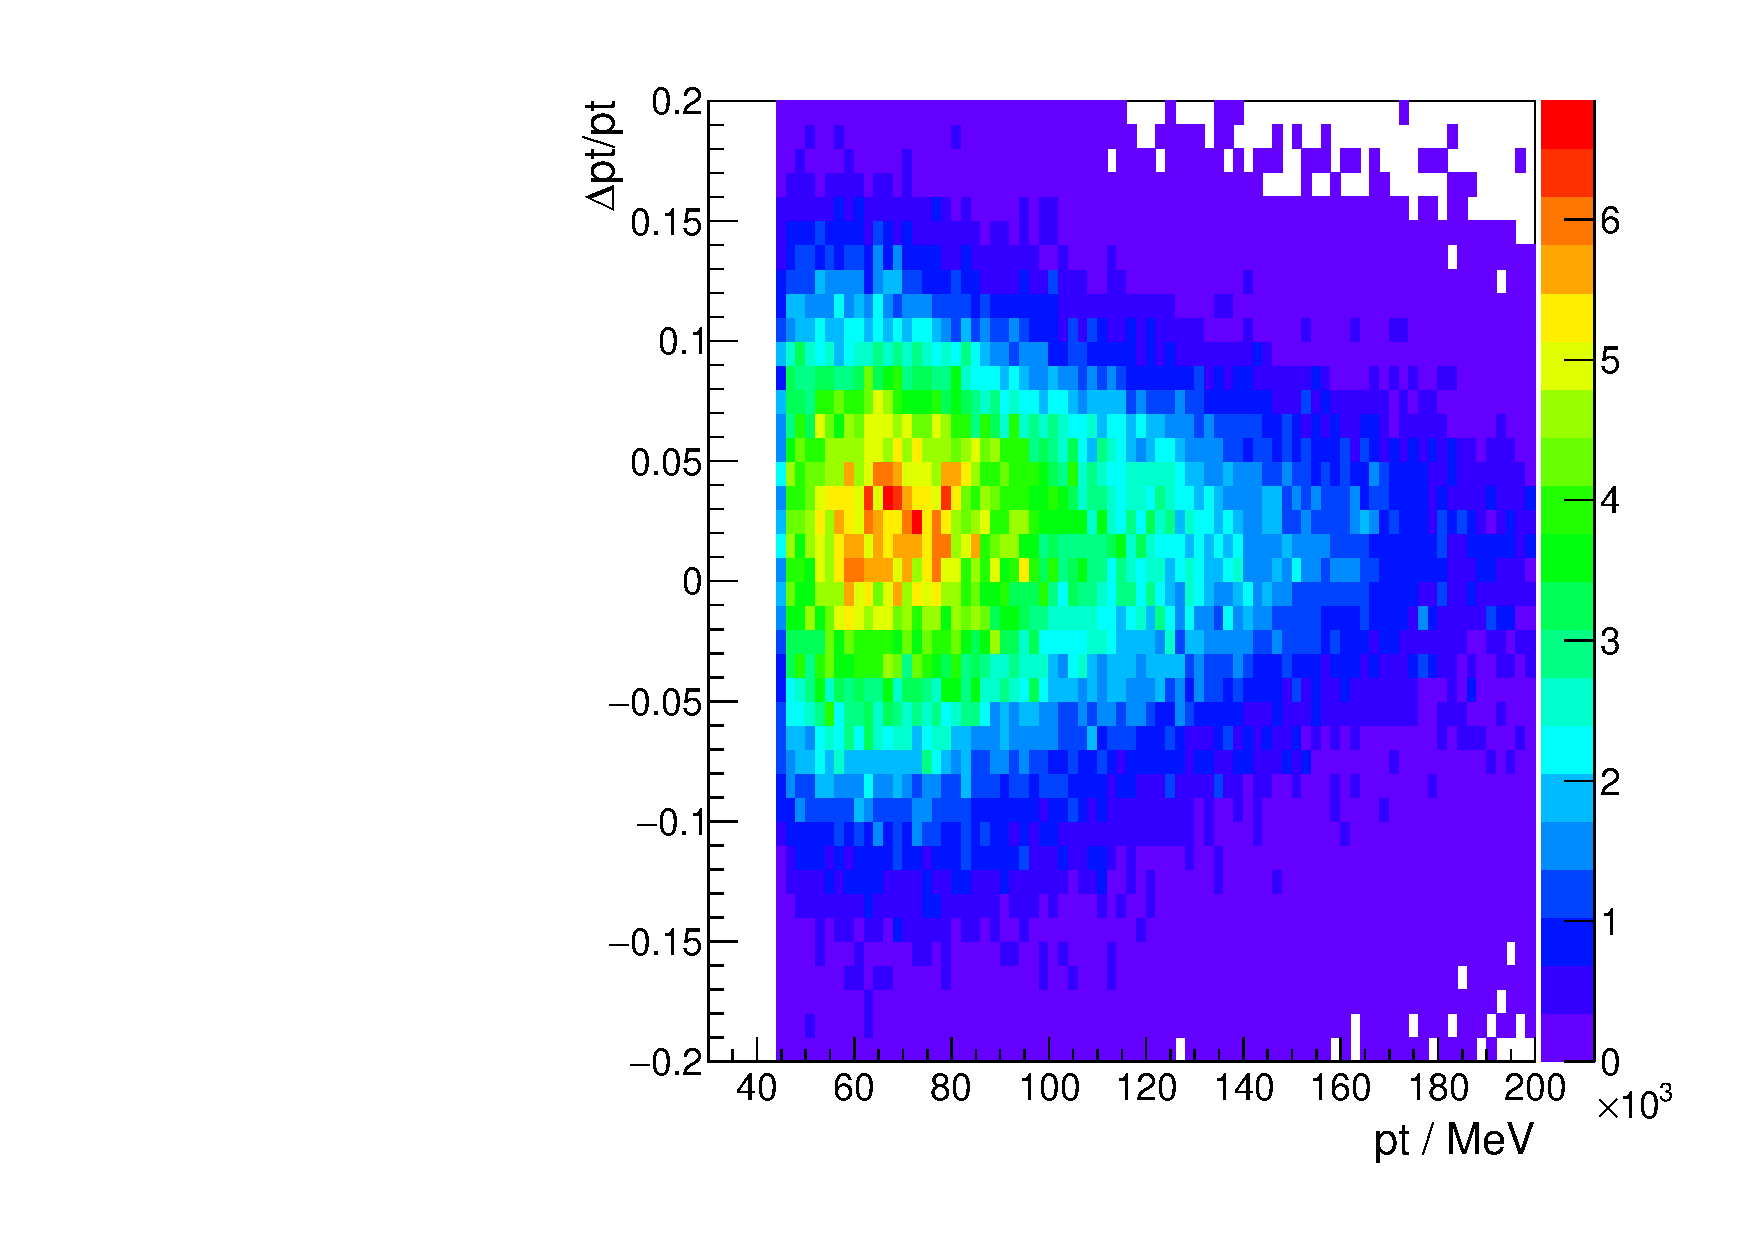
\includegraphics[width=1\linewidth]{ptRatio_Leading_BJet}

			\end{minipage}
			\quad
			\begin{minipage}[h]{0.33\linewidth}
				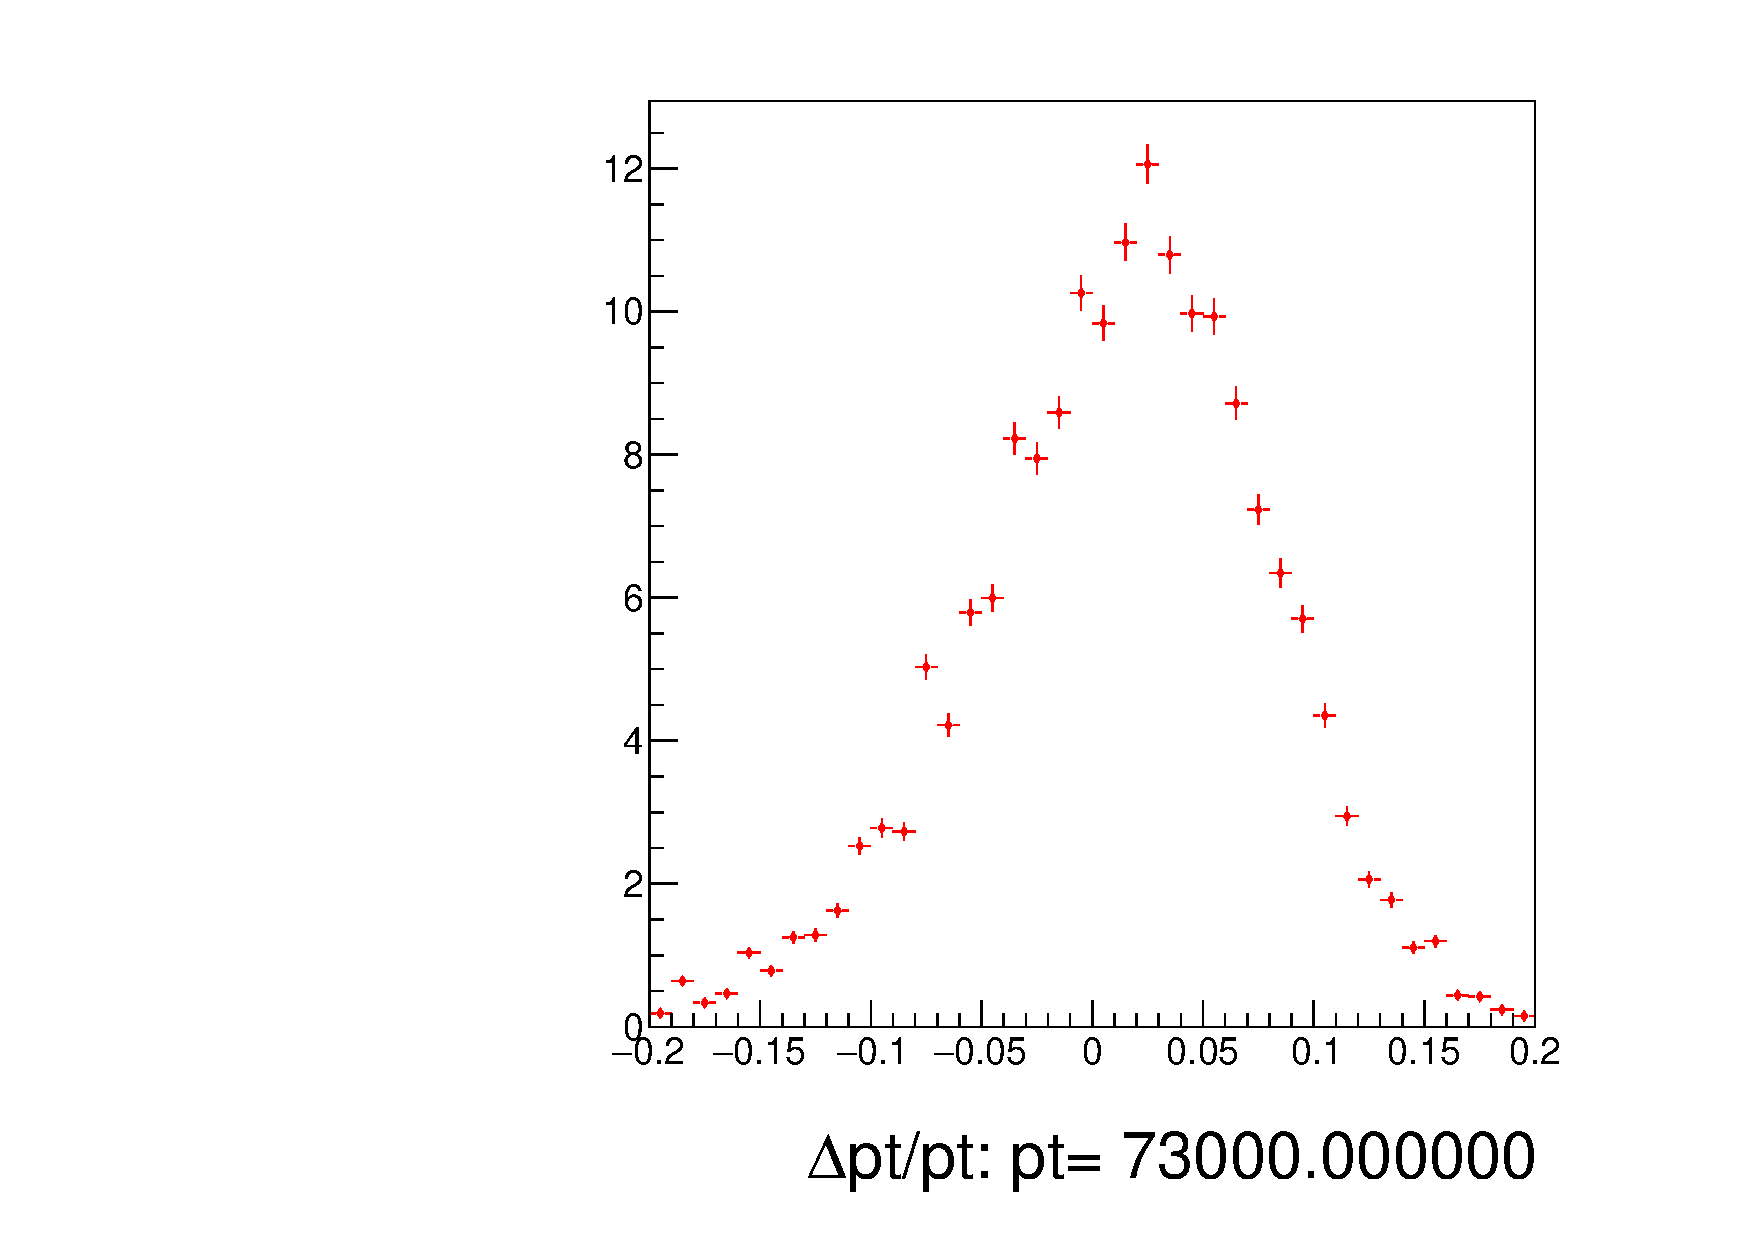
\includegraphics[width=1\linewidth]{ptRatio_Leading_BJet_Slice}
			\end{minipage}
			\caption{$\Delta $\pt$_{ratio}$ for the leading \pt $b$-jet from MC events against \pt of the offline $b$-jet. A slice across the $y$-axis has been taken at \pt$=79$GeV. }
			\label{fig:MC:leadingbpt}
		\end{figure}

		\begin{figure}[h]
			\centering

			\begin{minipage}[h]{0.33\linewidth}
				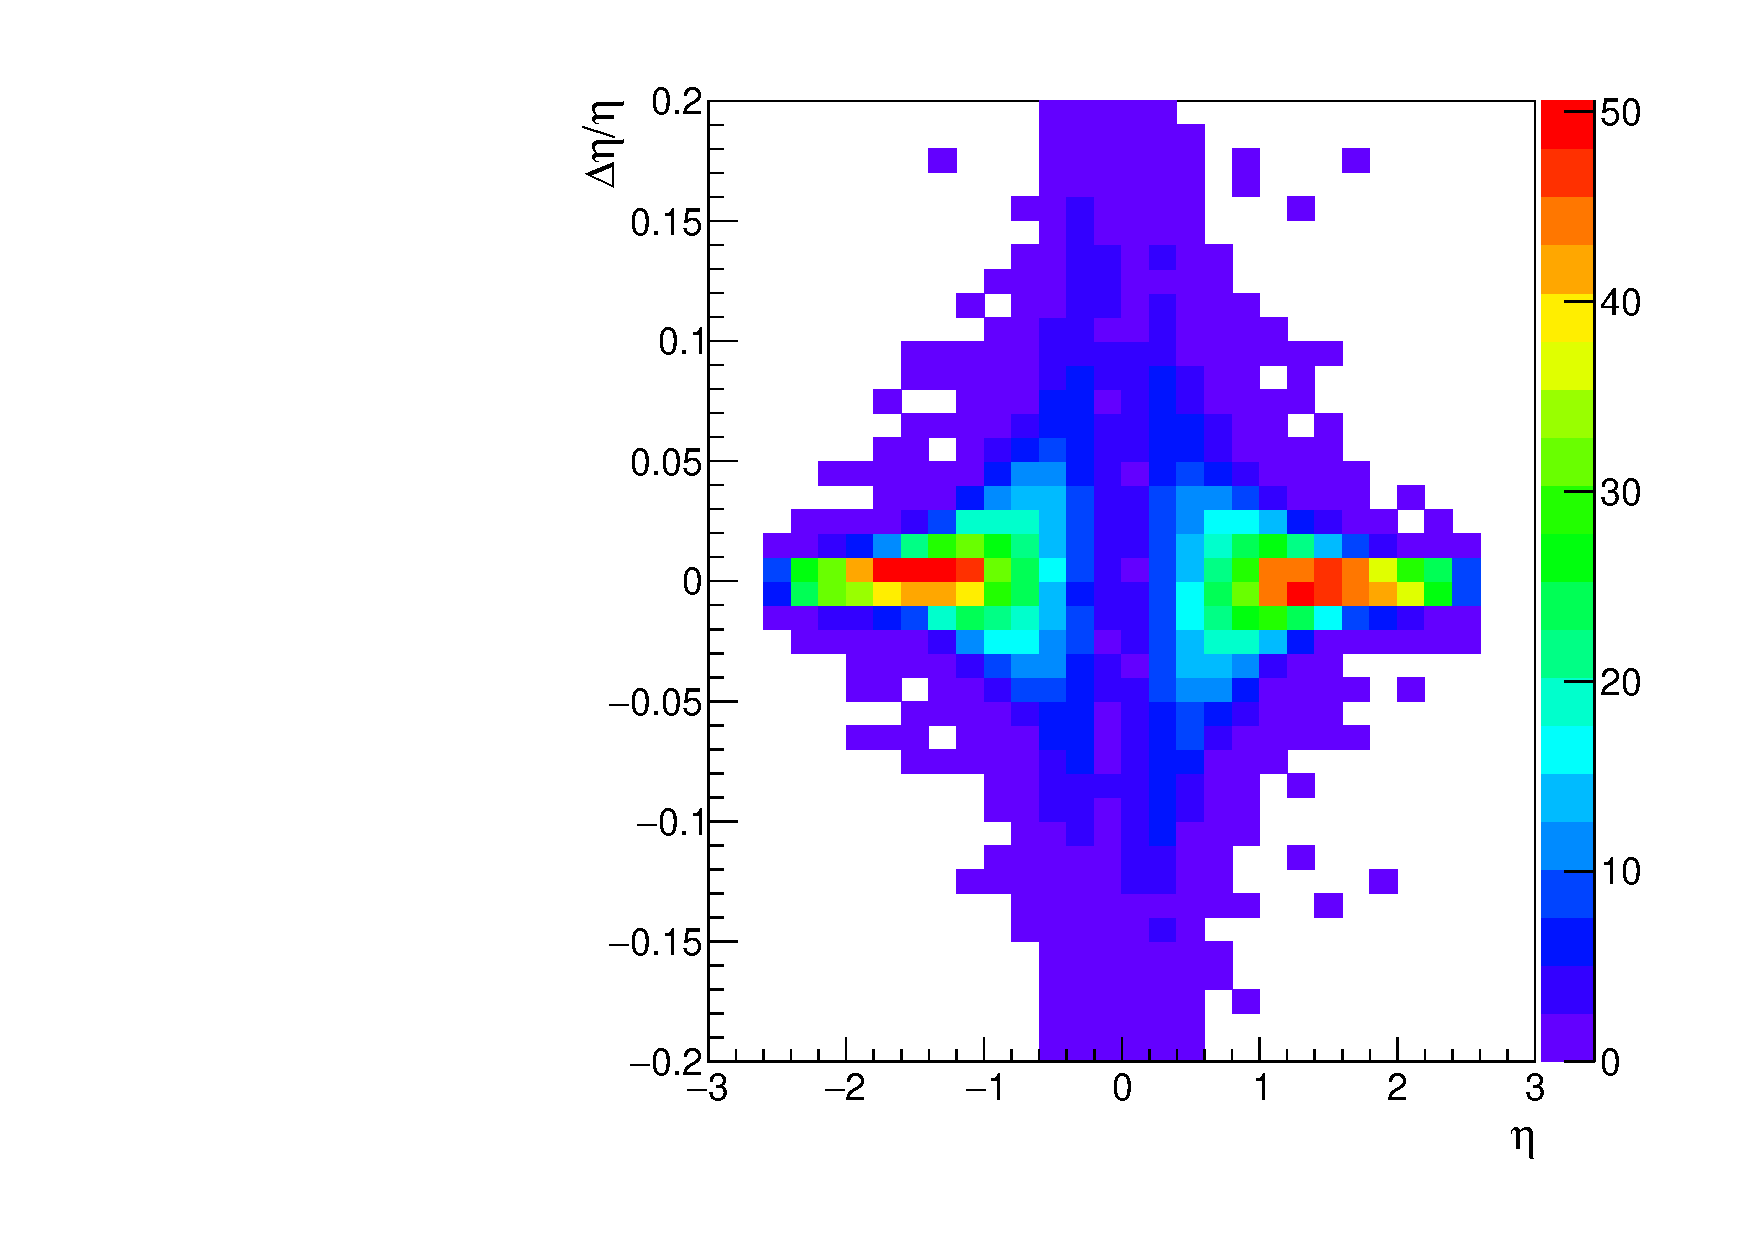
\includegraphics[width=1\linewidth]{etaRatio_Leading_BJet}
			\end{minipage}
			\quad
			\begin{minipage}[h]{0.33\linewidth}
				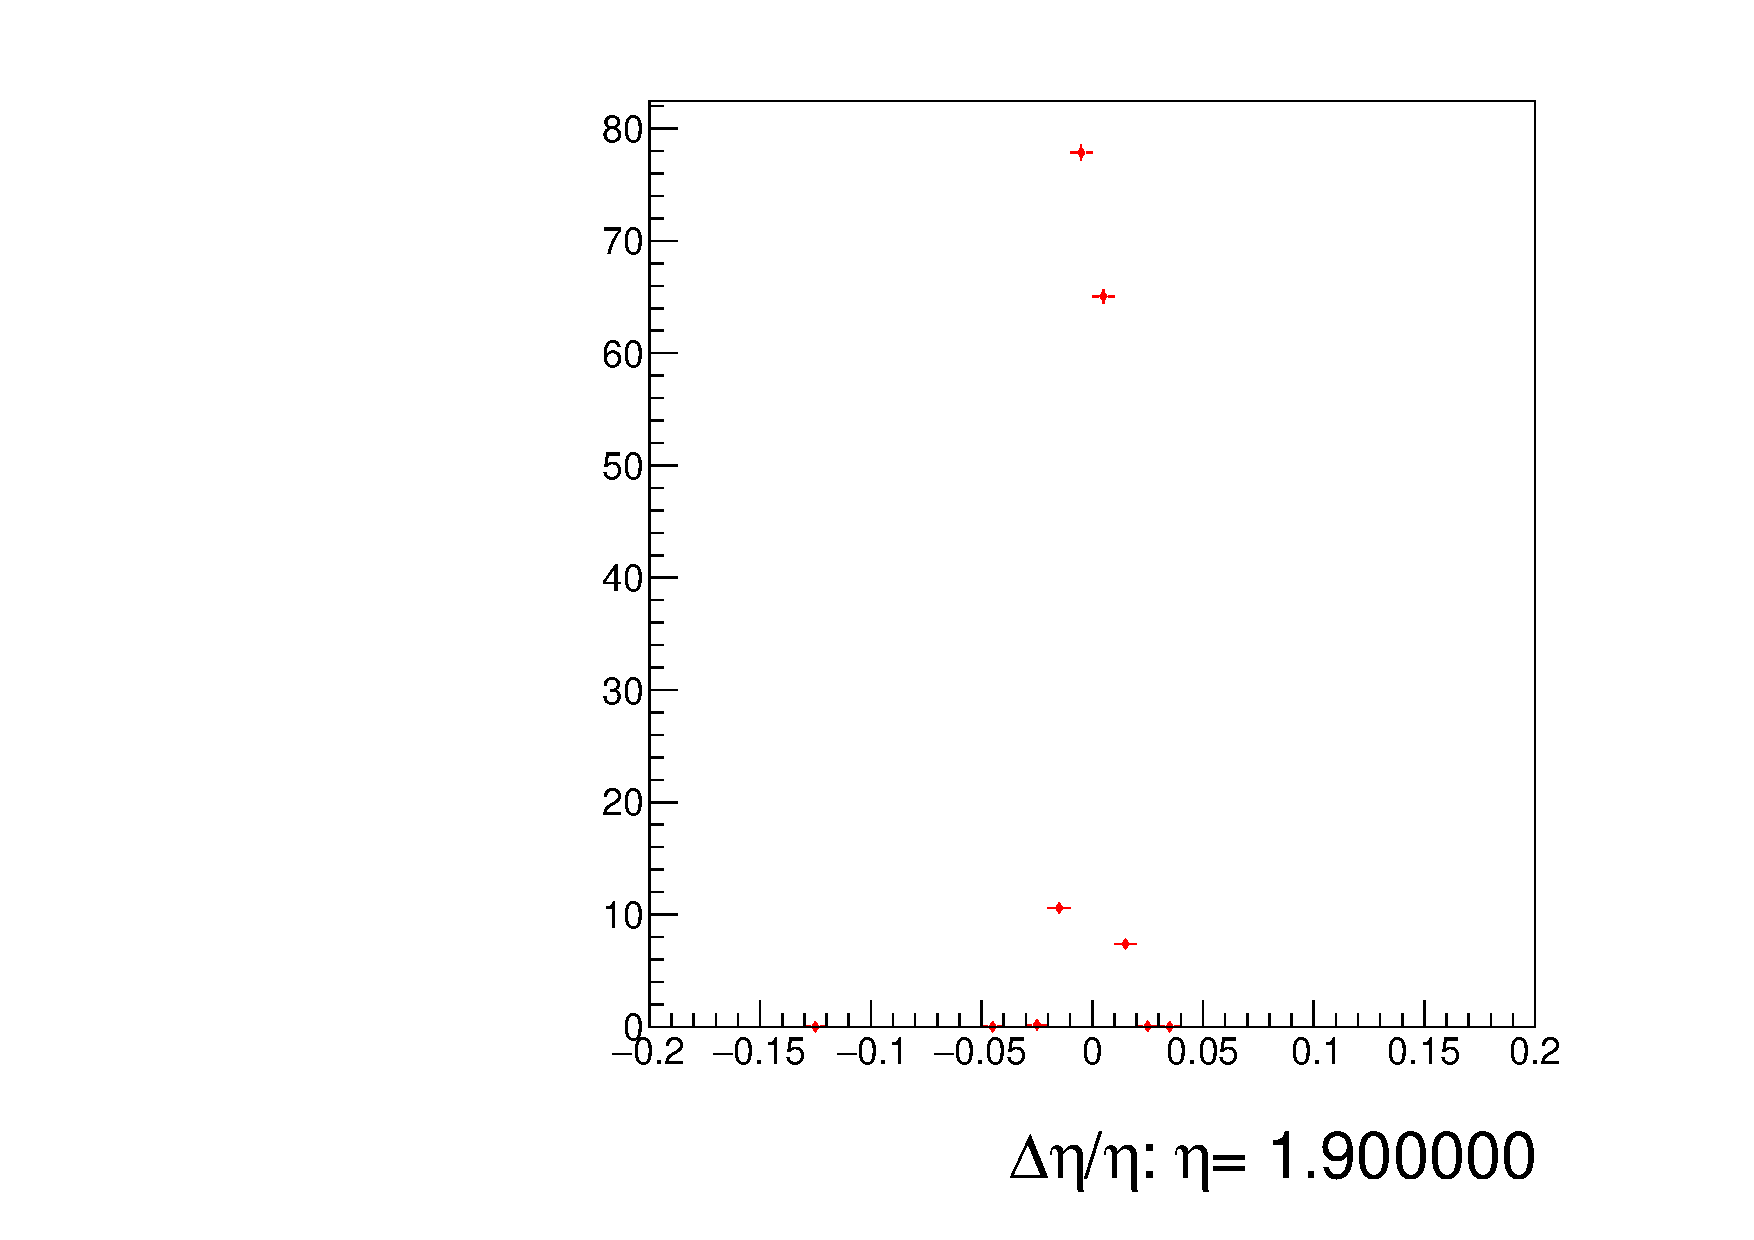
\includegraphics[width=1\linewidth]{etaRatio_Leading_BJet_Slice}
			\end{minipage}
			\caption{$\Delta \eta_{ratio}$ for the leading \pt $b$-jet from MC events against $\eta$ of the offline $b$-jet. A slice across the $y$-axis has been taken at $\eta=-1.9$. }
			\label{fig:MC:leadingbeta}
		\end{figure}

			\begin{figure}[h]
				\centering

				\begin{minipage}[h]{0.33\linewidth}
					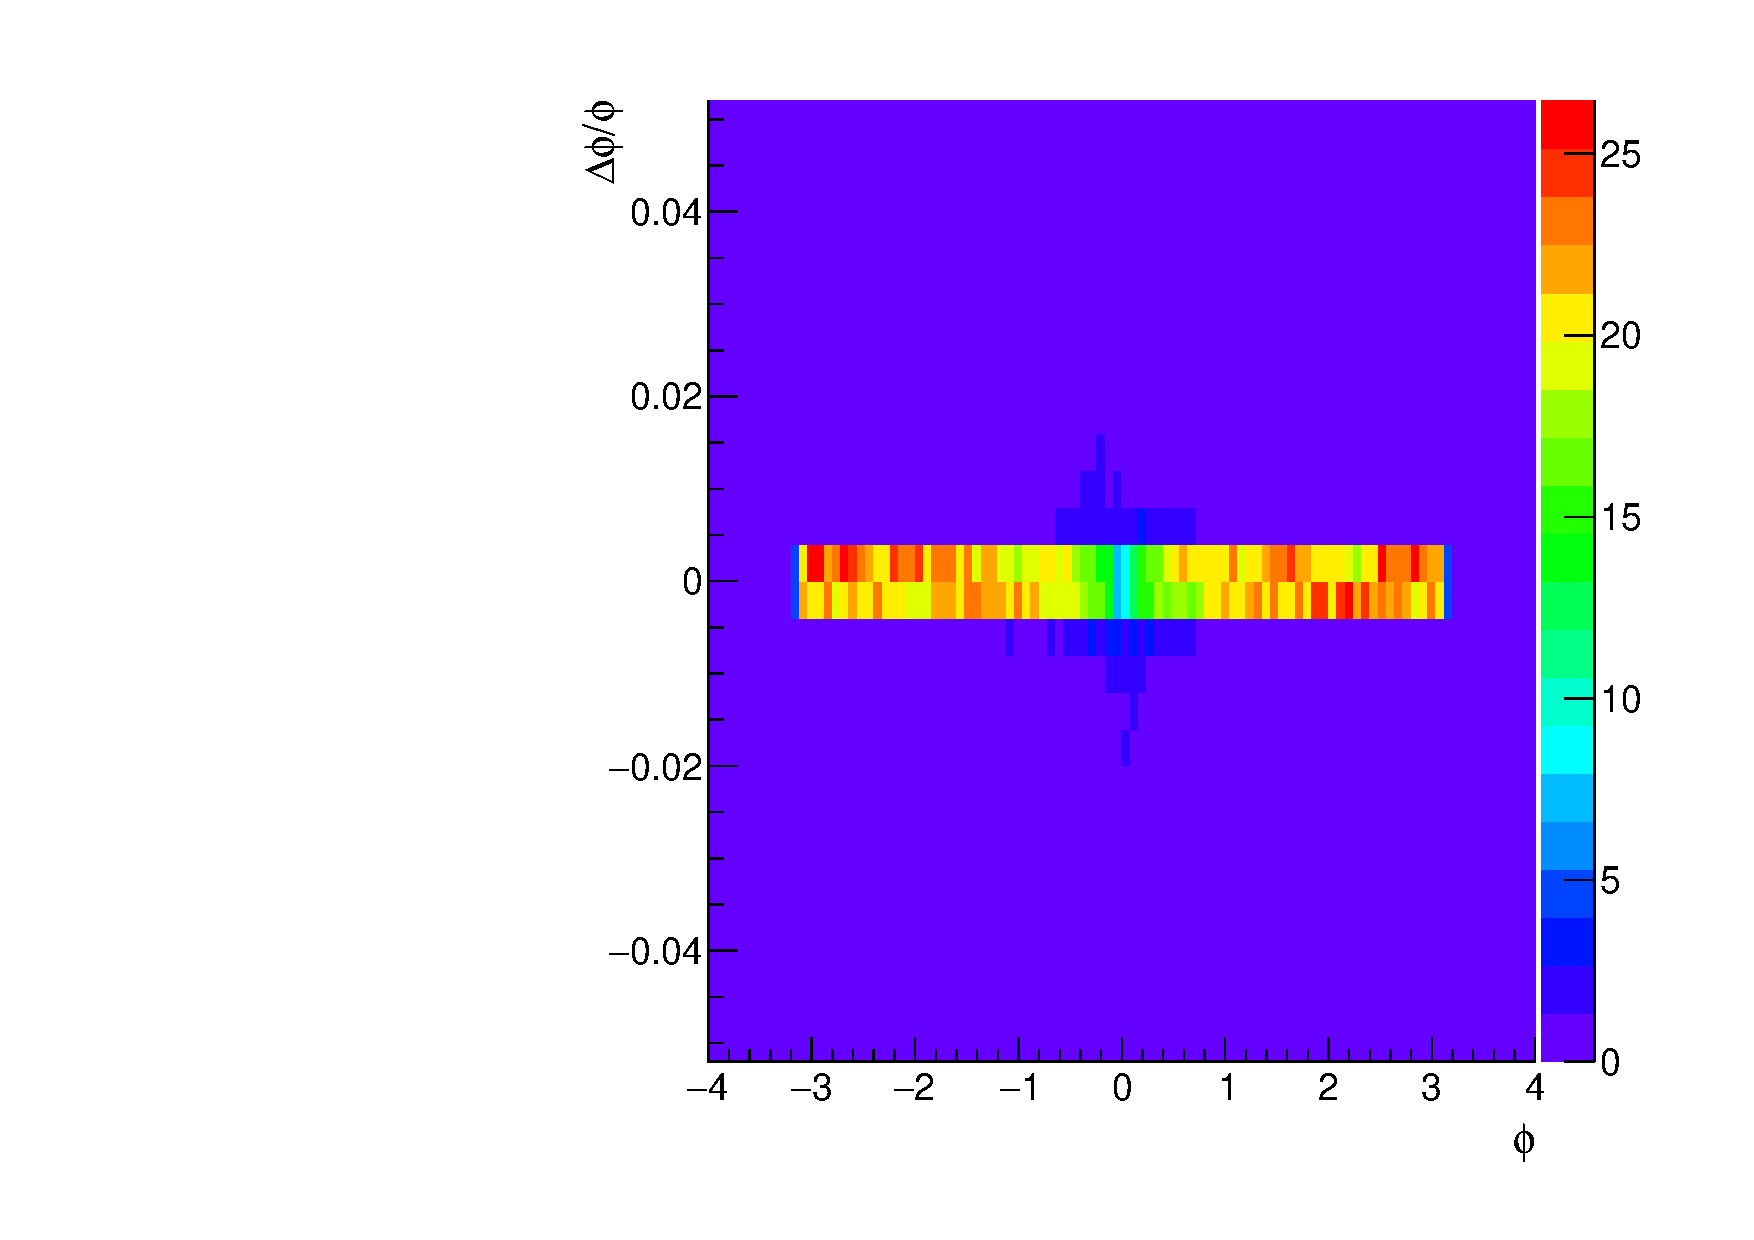
\includegraphics[width=1\linewidth]{phiRatio_Leading_BJet}
				\end{minipage}
				\quad
				\begin{minipage}[h]{0.33\linewidth}
					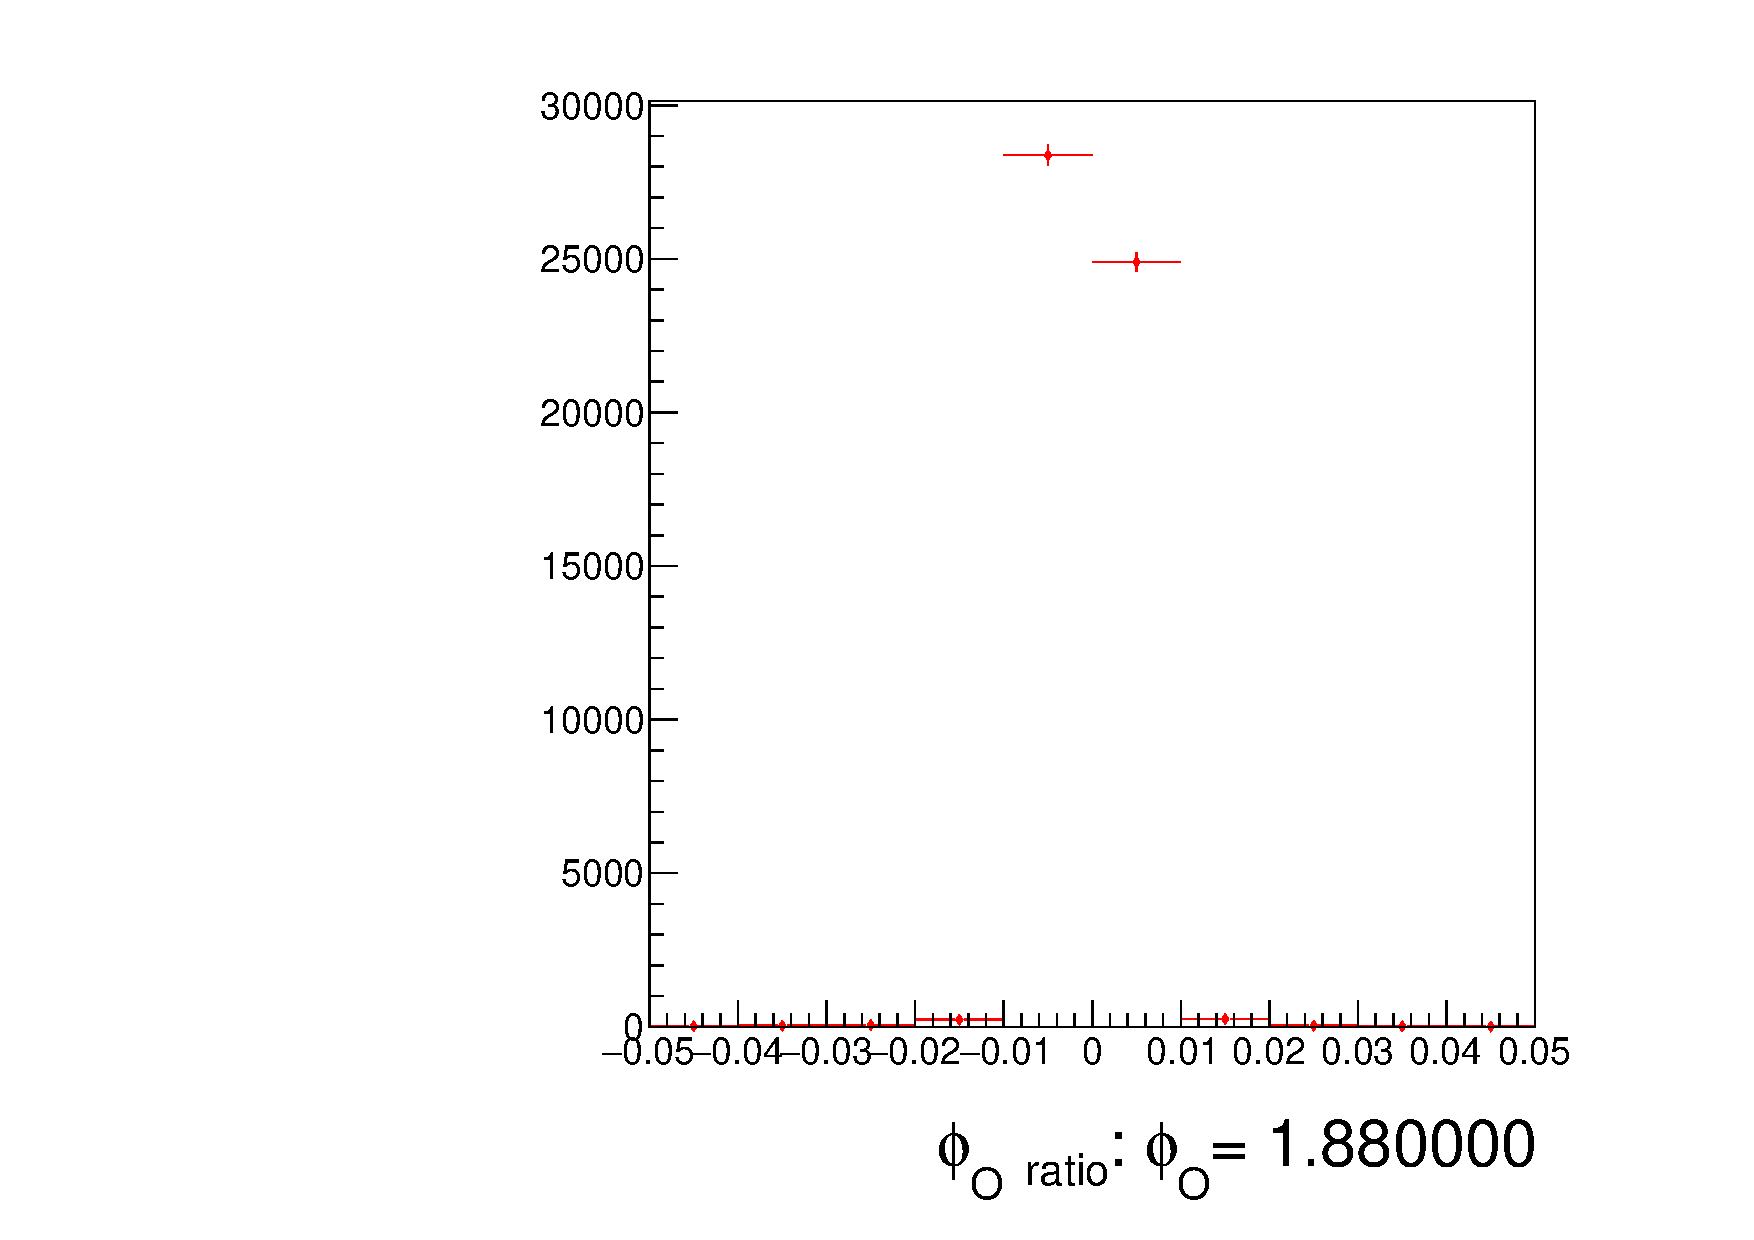
\includegraphics[width=1\linewidth]{phiRatio_Leading_BJet_Slice}
				\end{minipage}
			\caption{$\Delta \phi_{ratio}$ for the leading \pt $b$-jet from MC events against $\phi$ of the offline $b$-jet. A slice across the $y$-axis has been taken at $\phi=-1.64$. }
			\label{fig:MC:leadingbphi}
			\end{figure}

			\begin{figure}[h]
				\centering

				\begin{minipage}[h]{0.33\linewidth}
					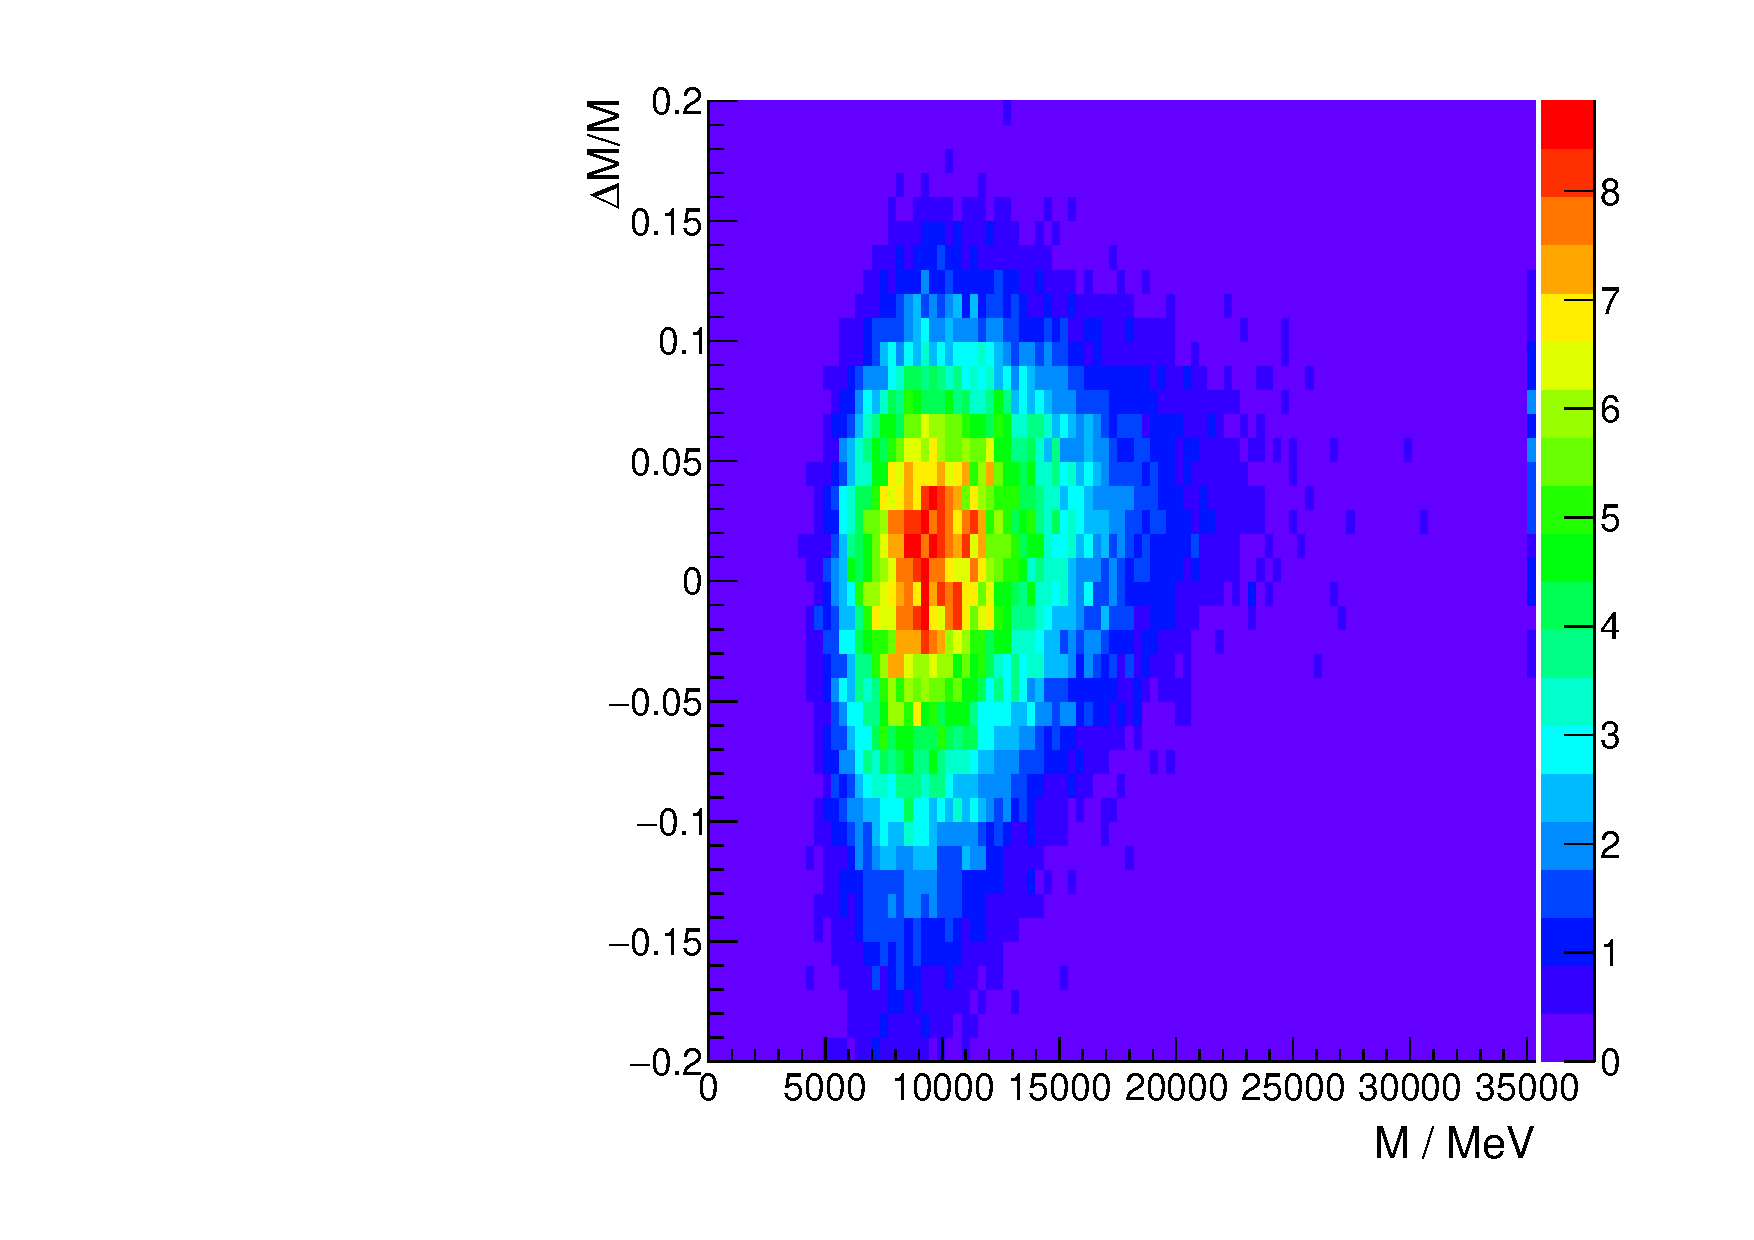
\includegraphics[width=1\linewidth]{mRatio_Leading_BJet}
				\end{minipage}
				\quad
				\begin{minipage}[h]{0.33\linewidth}
					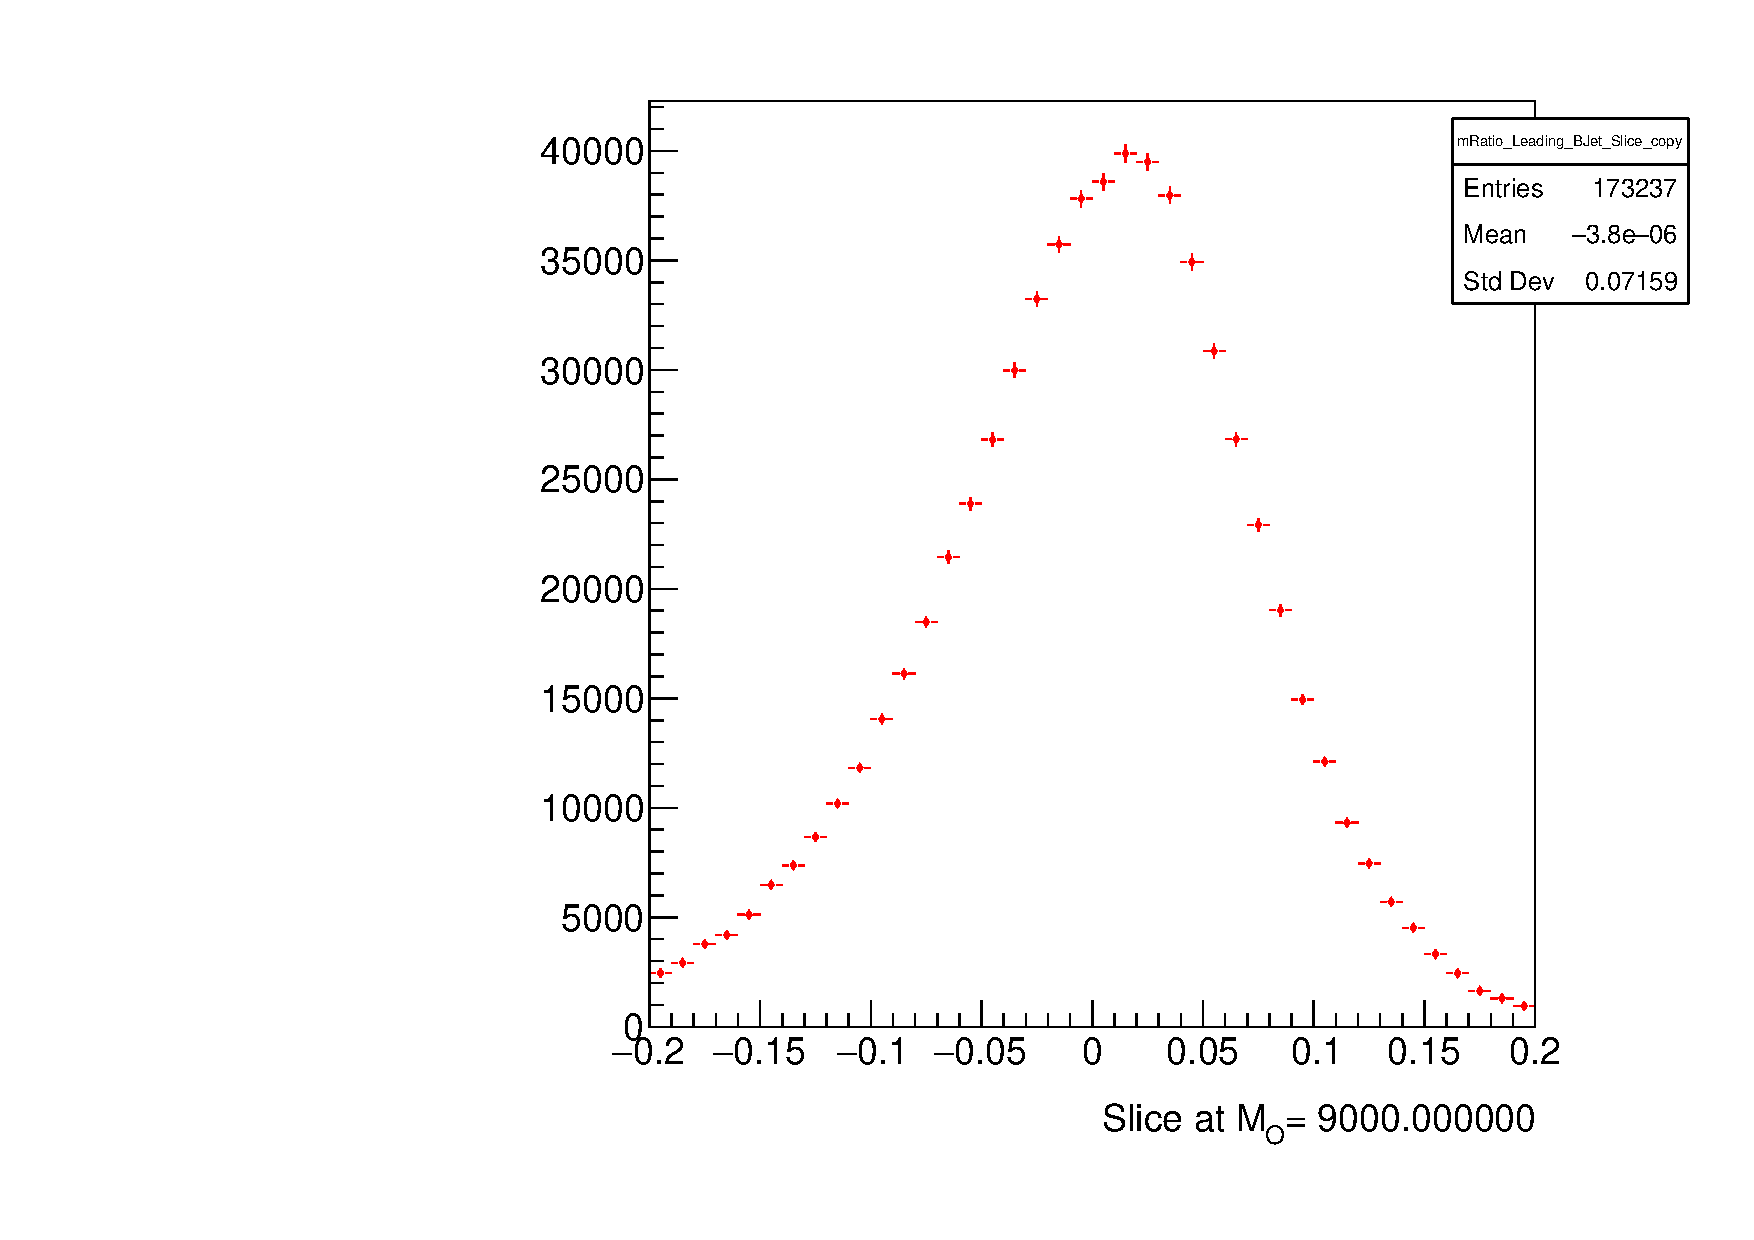
\includegraphics[width=1\linewidth]{mRatio_Leading_BJet_Slice}
				\end{minipage}
			\caption{$\Delta M_{ratio}$ for the leading \pt $b$-jet from MC events against $M$ of the offline $b$-jet. A slice across the $y$-axis has been taken at $M=7$GeV. }
			\label{fig:MC:leadingbm}
			\end{figure}

		\subsubsection{Conclusions from MC jet features}

	\newpage
	\subsection{Data}

		\begin{figure}[h]
			\centering
			\begin{minipage}[h]{0.33\linewidth}
				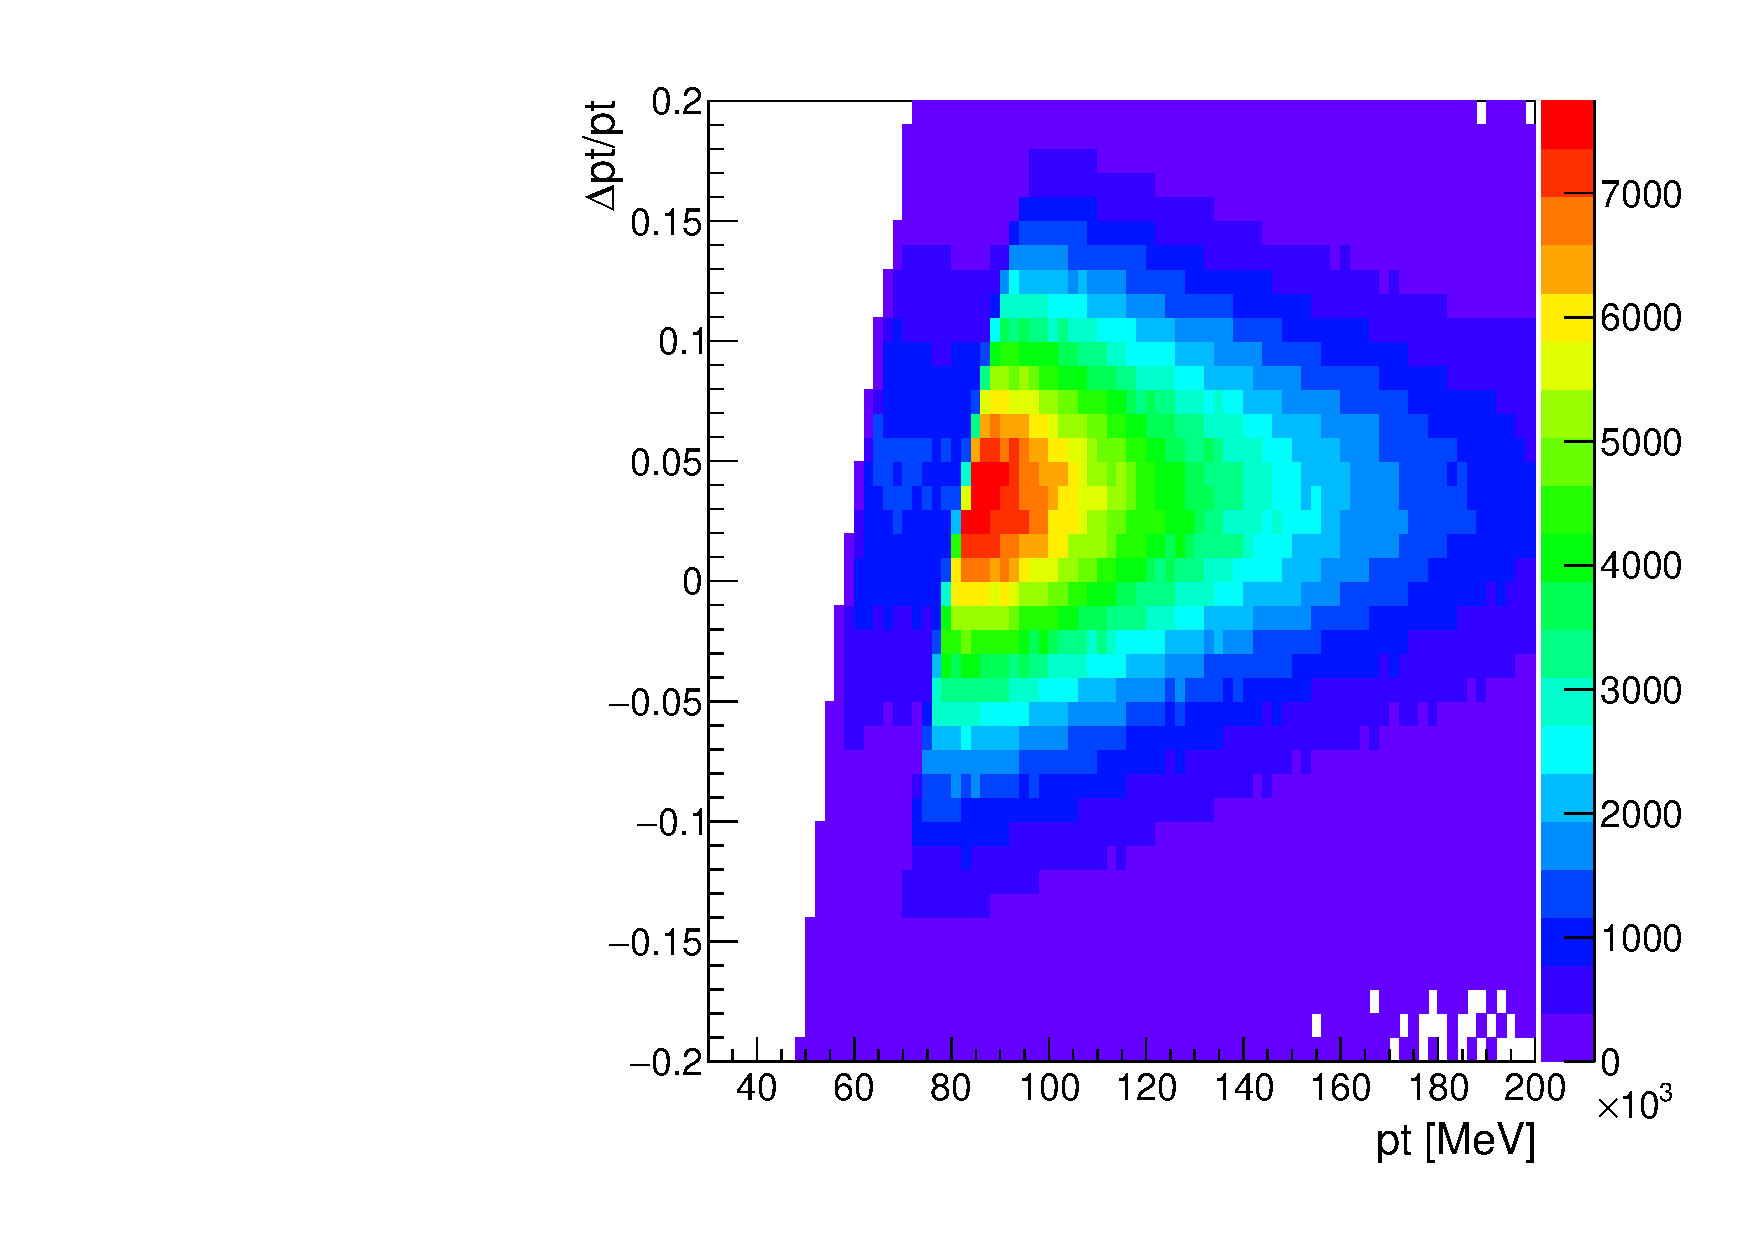
\includegraphics[width=1\linewidth]{Offline_2C_ptRatio_Leading_BJet}
				
			\end{minipage}
			\quad
			\begin{minipage}[h]{0.33\linewidth}
				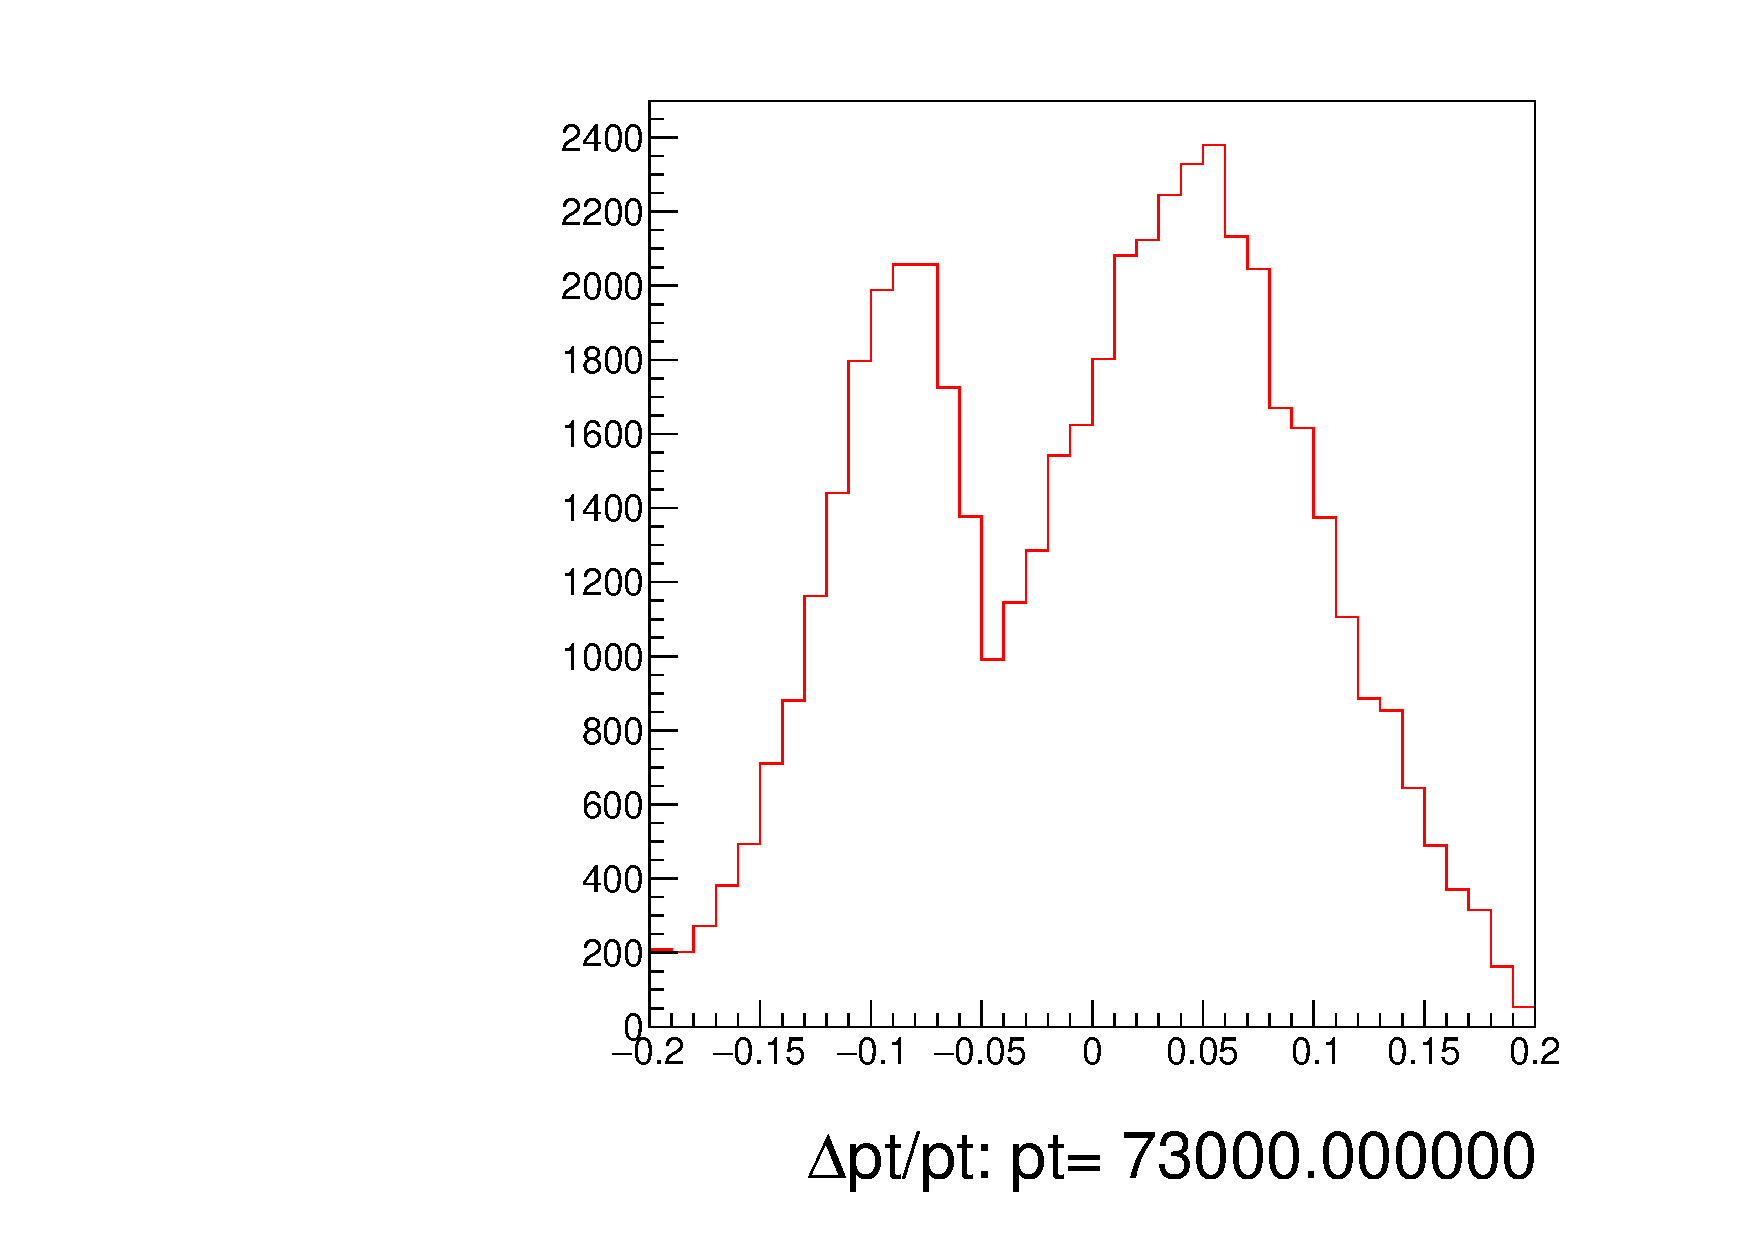
\includegraphics[width=1\linewidth]{Offline_2C_ptRatio_Leading_BJet_Slice}
			\end{minipage}
			\caption{$\Delta $\pt$_{ratio}$ for the leading \pt $b$-jet from data events against \pt of the offline $b$-jet. A slice across the $y$-axis has been taken at \pt$=79$GeV. }
			\label{fig:D:leadingbpt}
		\end{figure}
		
		\begin{figure}[h]
			\centering
			
			\begin{minipage}[h]{0.33\linewidth}
				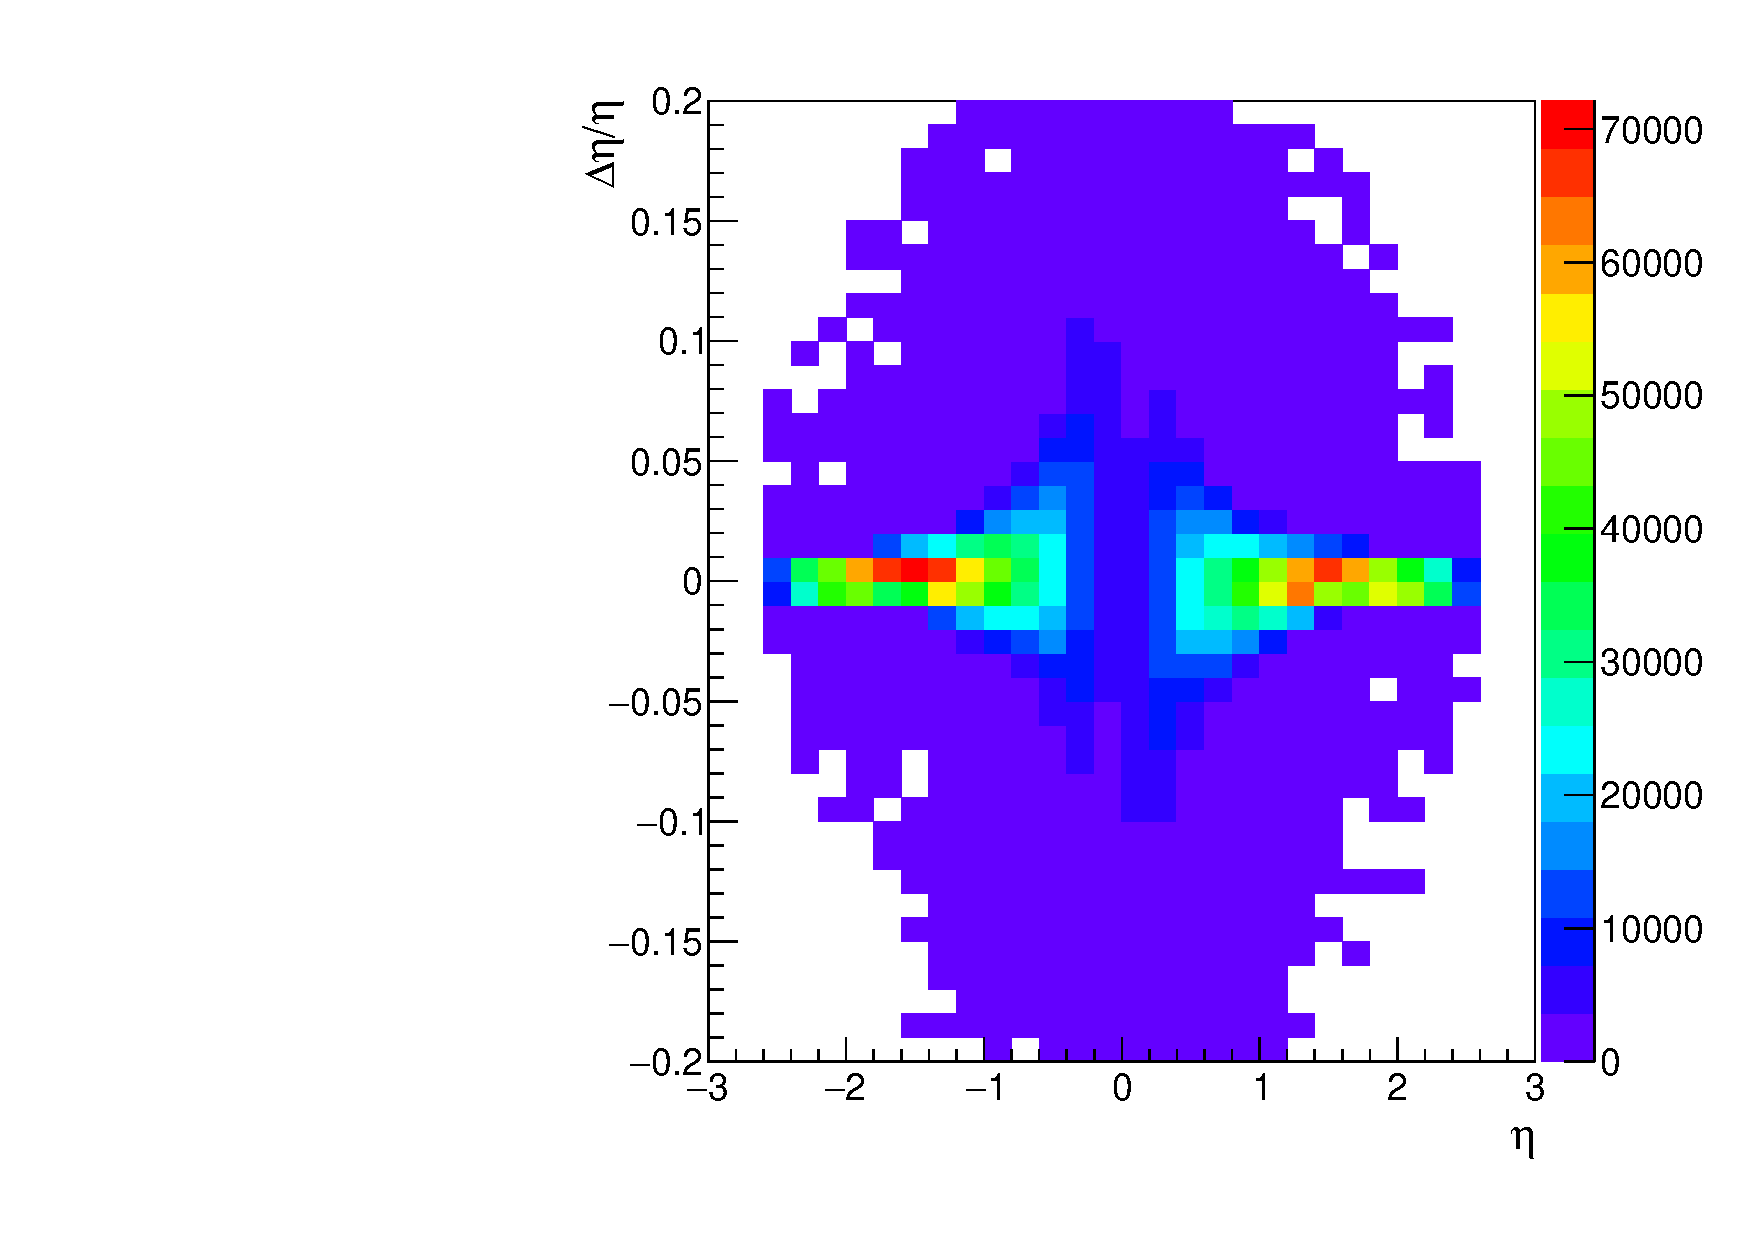
\includegraphics[width=1\linewidth]{Offline_2C_etaRatio_Leading_BJet}
			\end{minipage}
			\quad
			\begin{minipage}[h]{0.33\linewidth}
				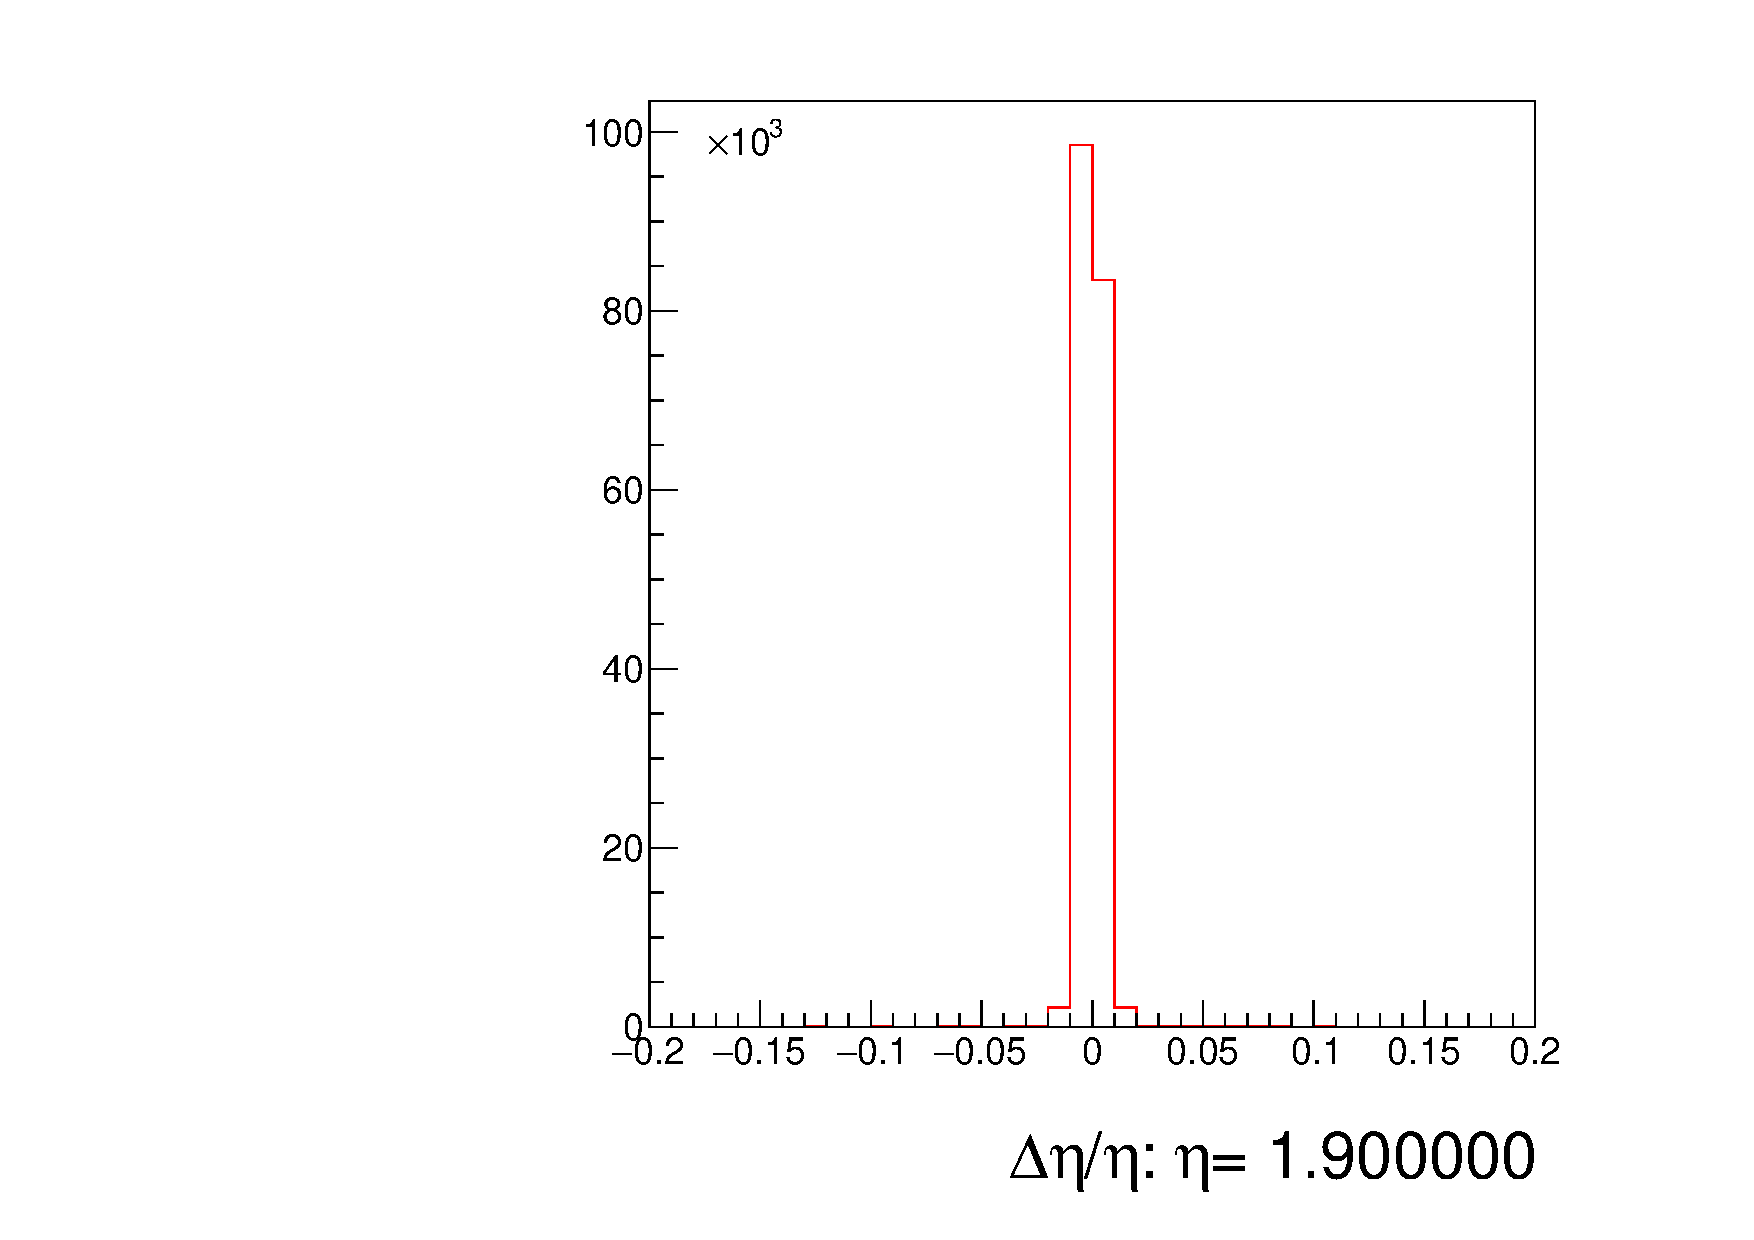
\includegraphics[width=1\linewidth]{Offline_2C_etaRatio_Leading_BJet_Slice}
			\end{minipage}
			\caption{$\Delta \eta_{ratio}$ for the leading \pt $b$-jet from  data events against $\eta$ of the offline $b$-jet. A slice across the $y$-axis has been taken at $\eta=-1.9$. }
			\label{fig:D:leadingbeta}
		\end{figure}
		
		\begin{figure}[h]
			\centering
			
			\begin{minipage}[h]{0.33\linewidth}
				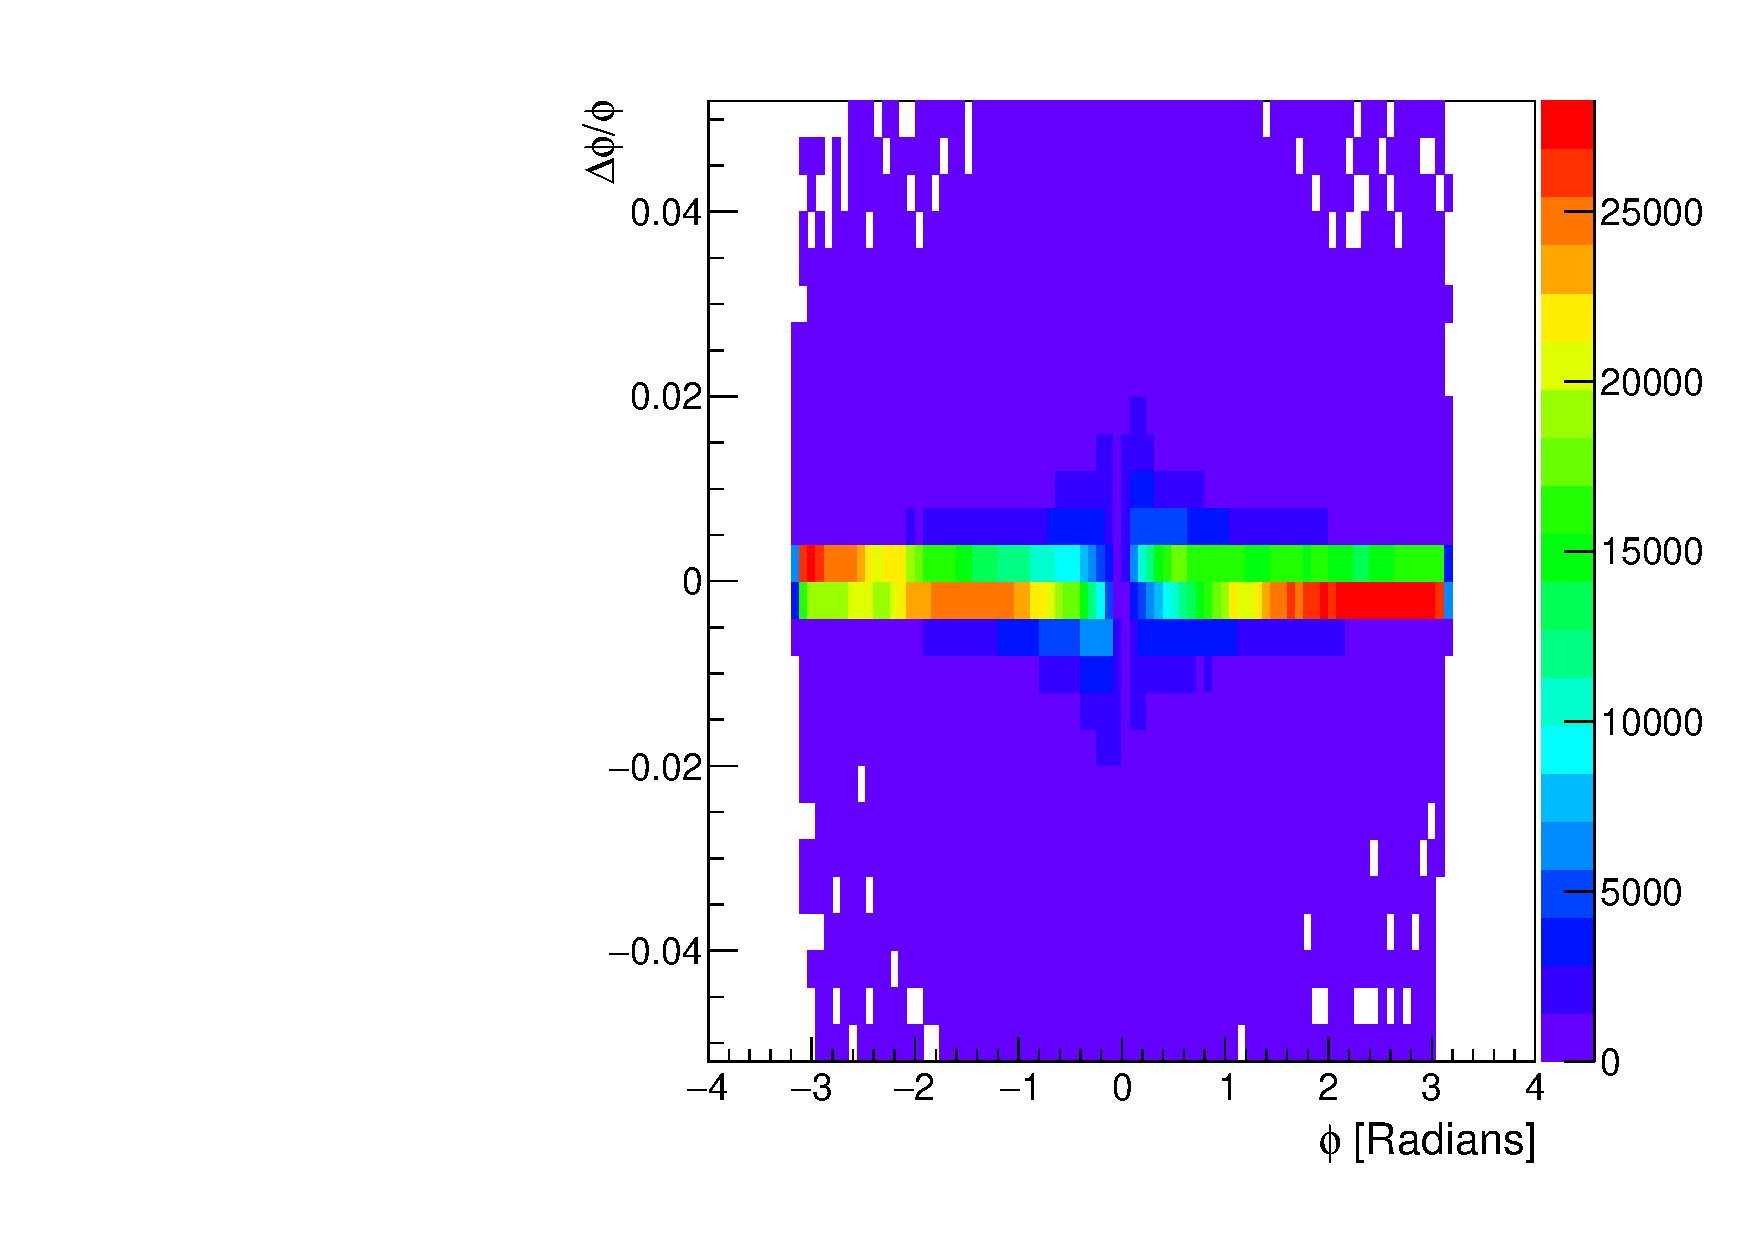
\includegraphics[width=1\linewidth]{Offline_2C_phiRatio_Leading_BJet}
			\end{minipage}
			\quad
			\begin{minipage}[h]{0.33\linewidth}
				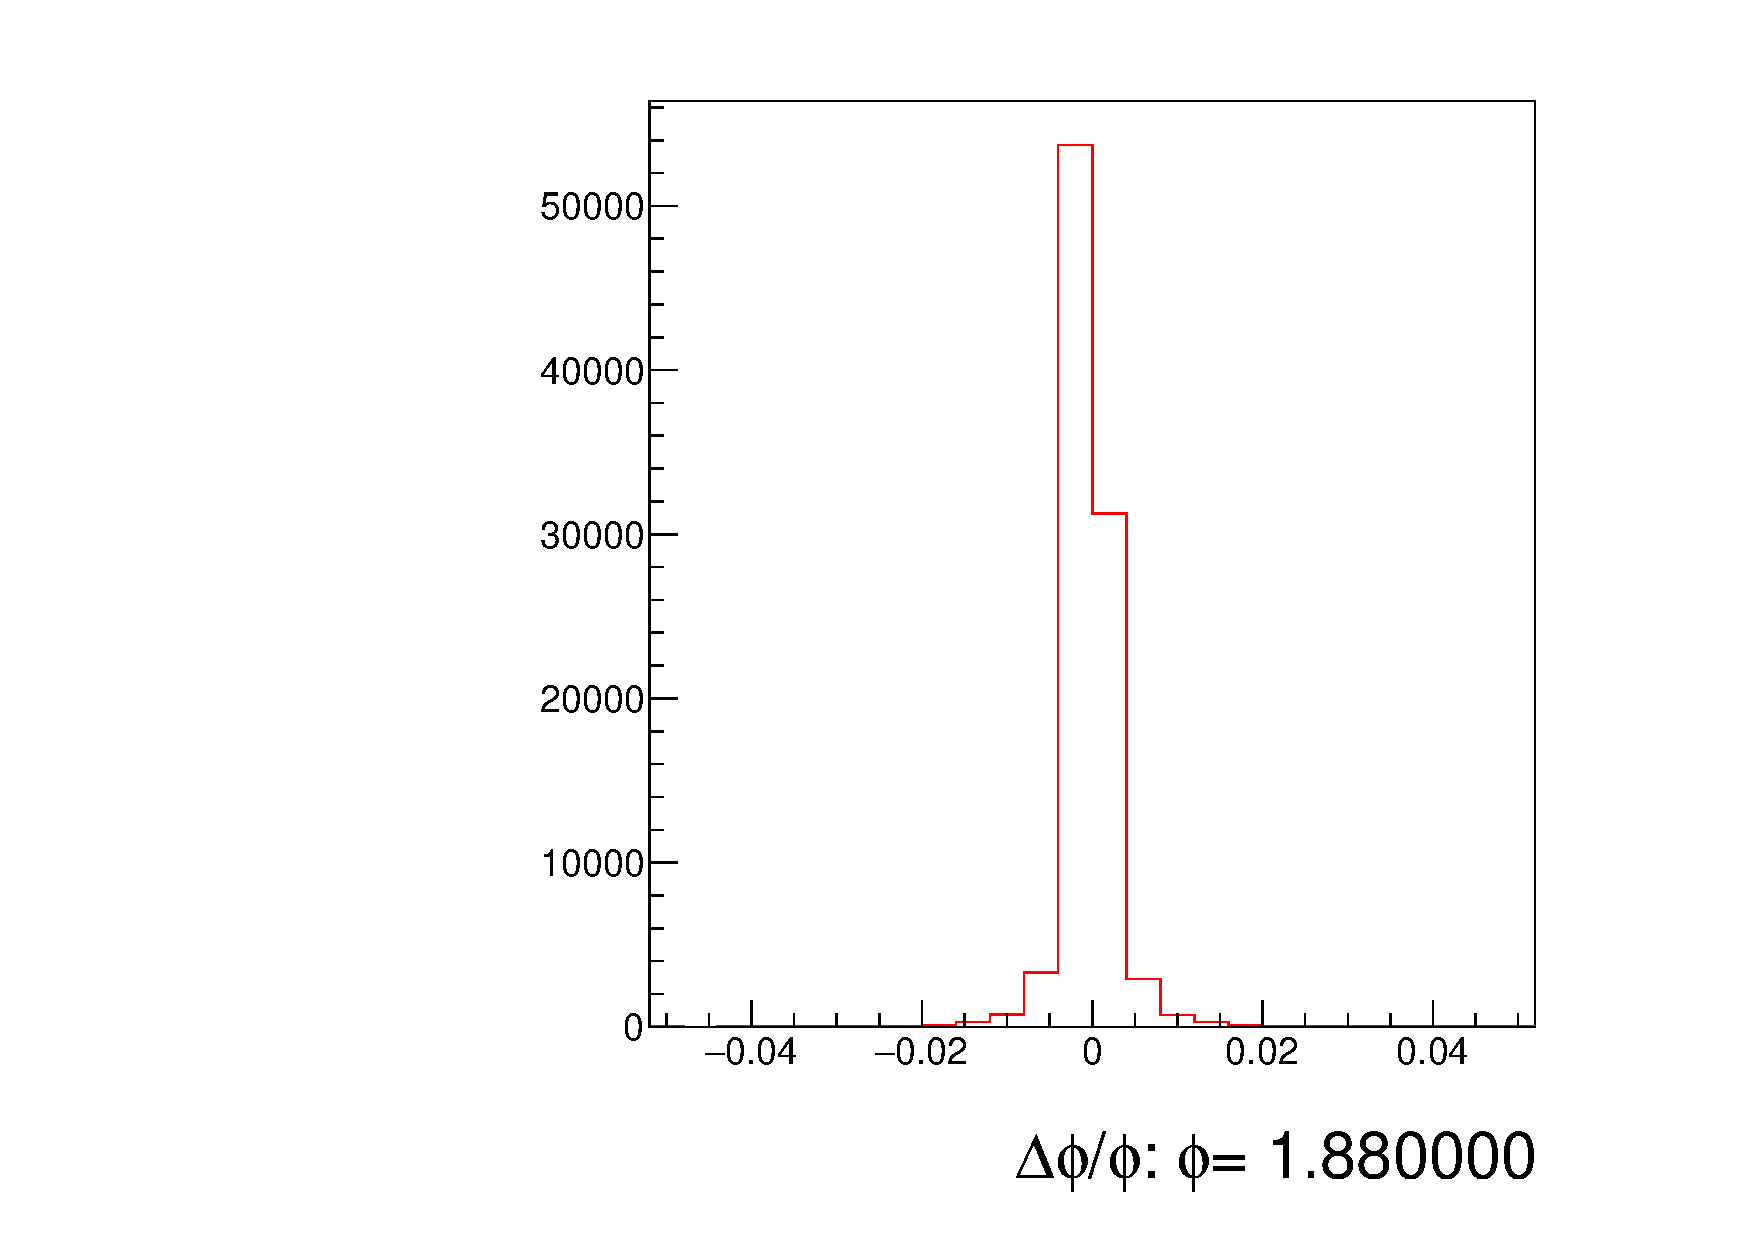
\includegraphics[width=1\linewidth]{Offline_2C_phiRatio_Leading_BJet_Slice}
			\end{minipage}
			\caption{$\Delta \phi_{ratio}$ for the leading \pt $b$-jet from  data events against $\phi$ of the offline $b$-jet. A slice across the $y$-axis has been taken at $\phi=-1.64$. }
			\label{fig:D:leadingbphi}
		\end{figure}
		
		\begin{figure}[h]
			\centering
			
			\begin{minipage}[h]{0.33\linewidth}
				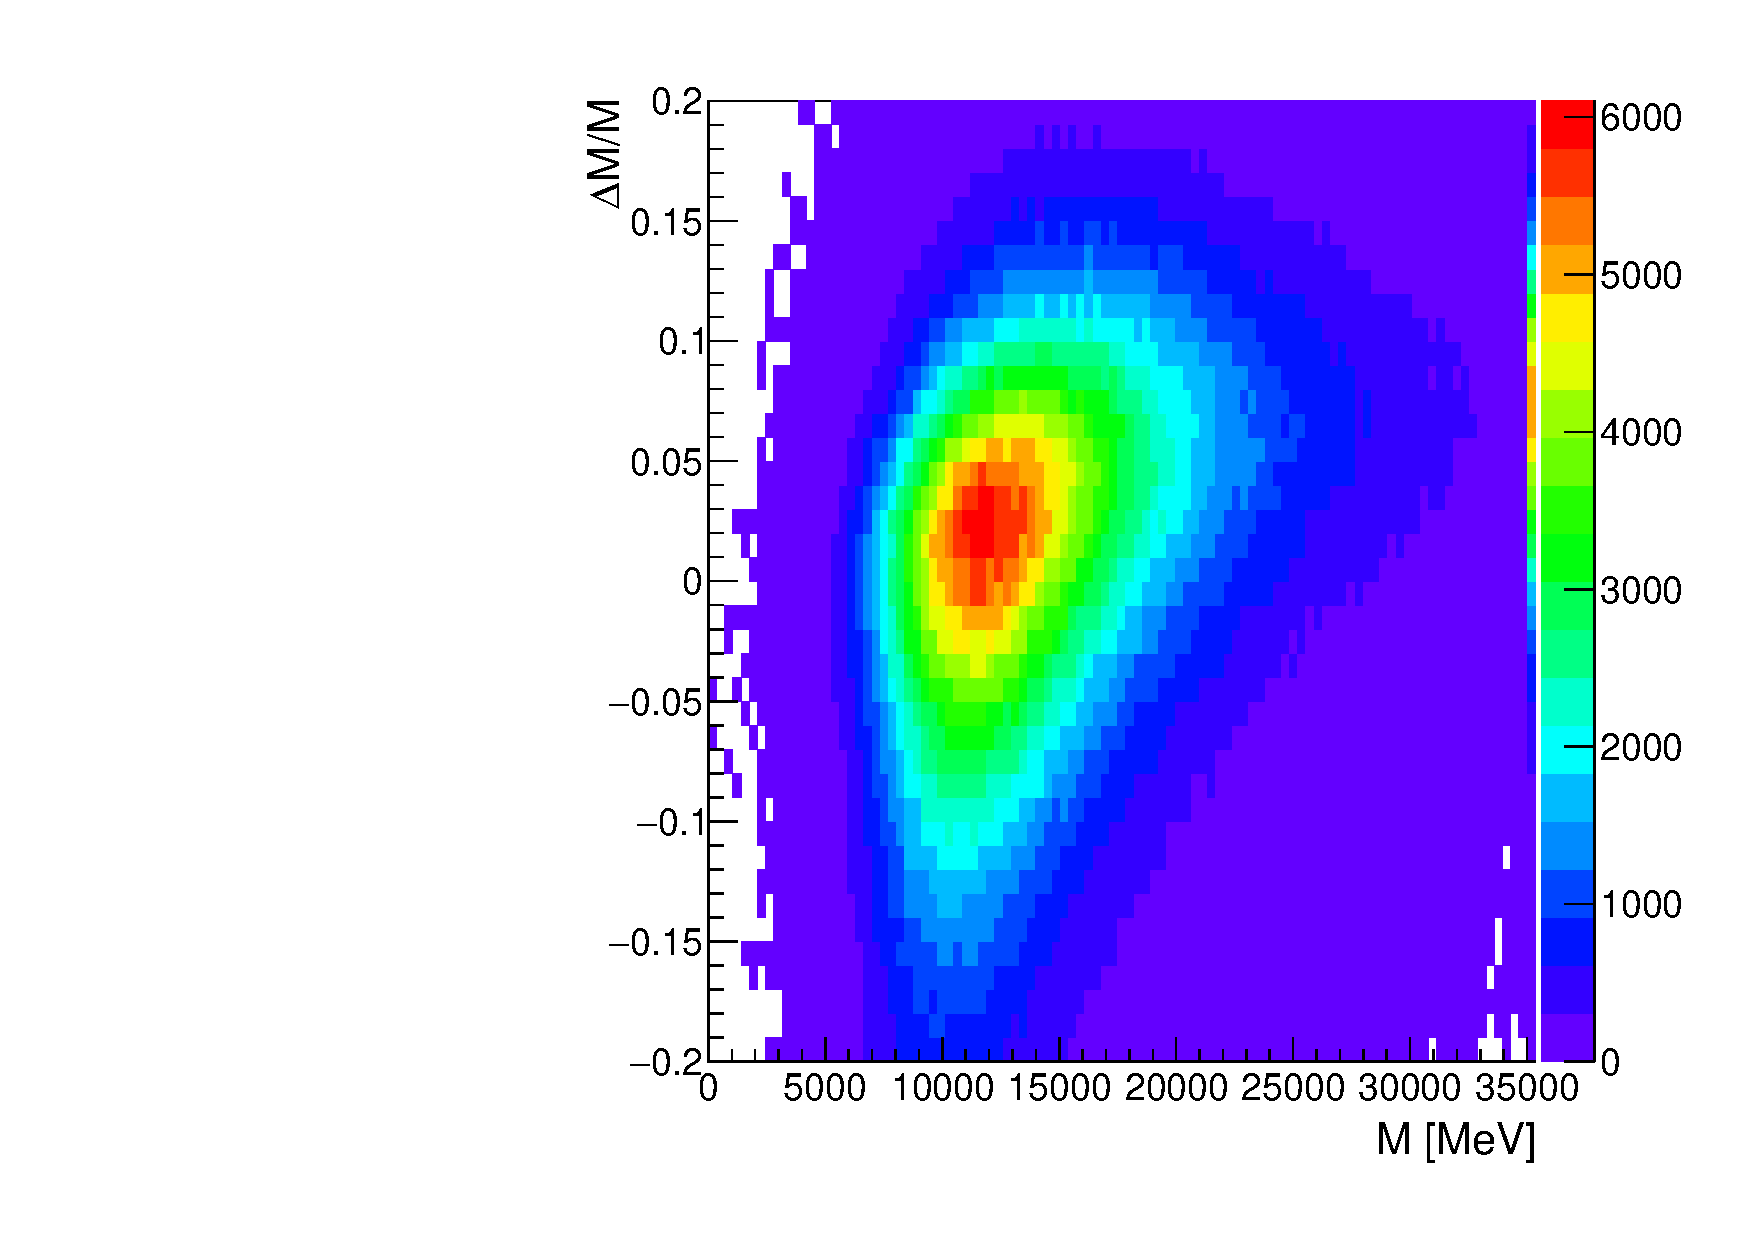
\includegraphics[width=1\linewidth]{Offline_2C_mRatio_Leading_BJet}
			\end{minipage}
			\quad
			\begin{minipage}[h]{0.33\linewidth}
				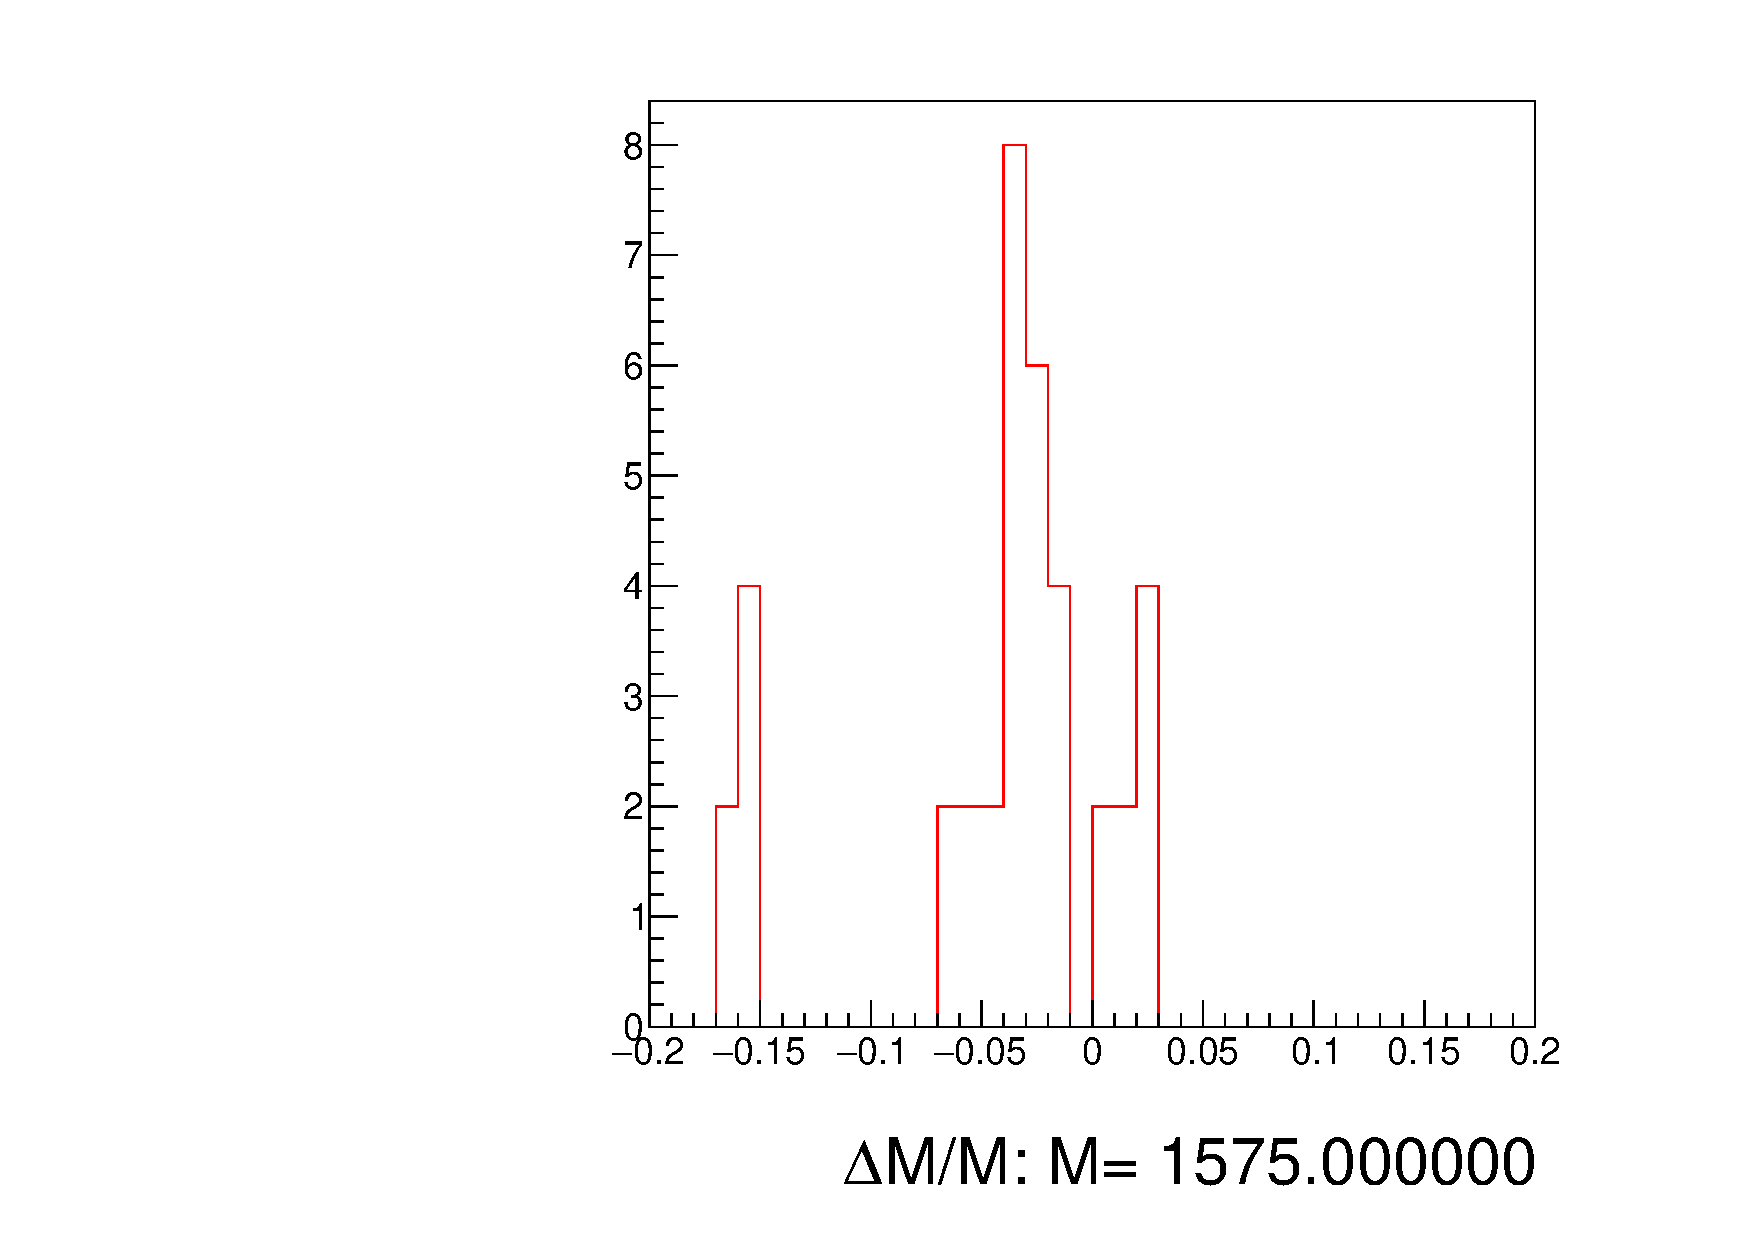
\includegraphics[width=1\linewidth]{Offline_2C_mRatio_Leading_BJet_Slice}
			\end{minipage}
			\caption{$\Delta M_{ratio}$ for the leading \pt $b$-jet from  data events against $M$ of the offline $b$-jet. A slice across the $y$-axis has been taken at $M=7$GeV. }
			\label{fig:D:leadingbm}
		\end{figure}

\newpage
\section{Leading Non \textit{b}-jets}

	The non $b$-jet category is defined as the jets exclusive to those tagged in Section \ref{OP:leadingb}. Again, the leading \pt offline jet from this list is matched with an online jet for the comparison.

	\subsection{Monte-Carlo}

		\begin{figure}[h]
			\centering
			\begin{minipage}[h]{0.33\linewidth}
				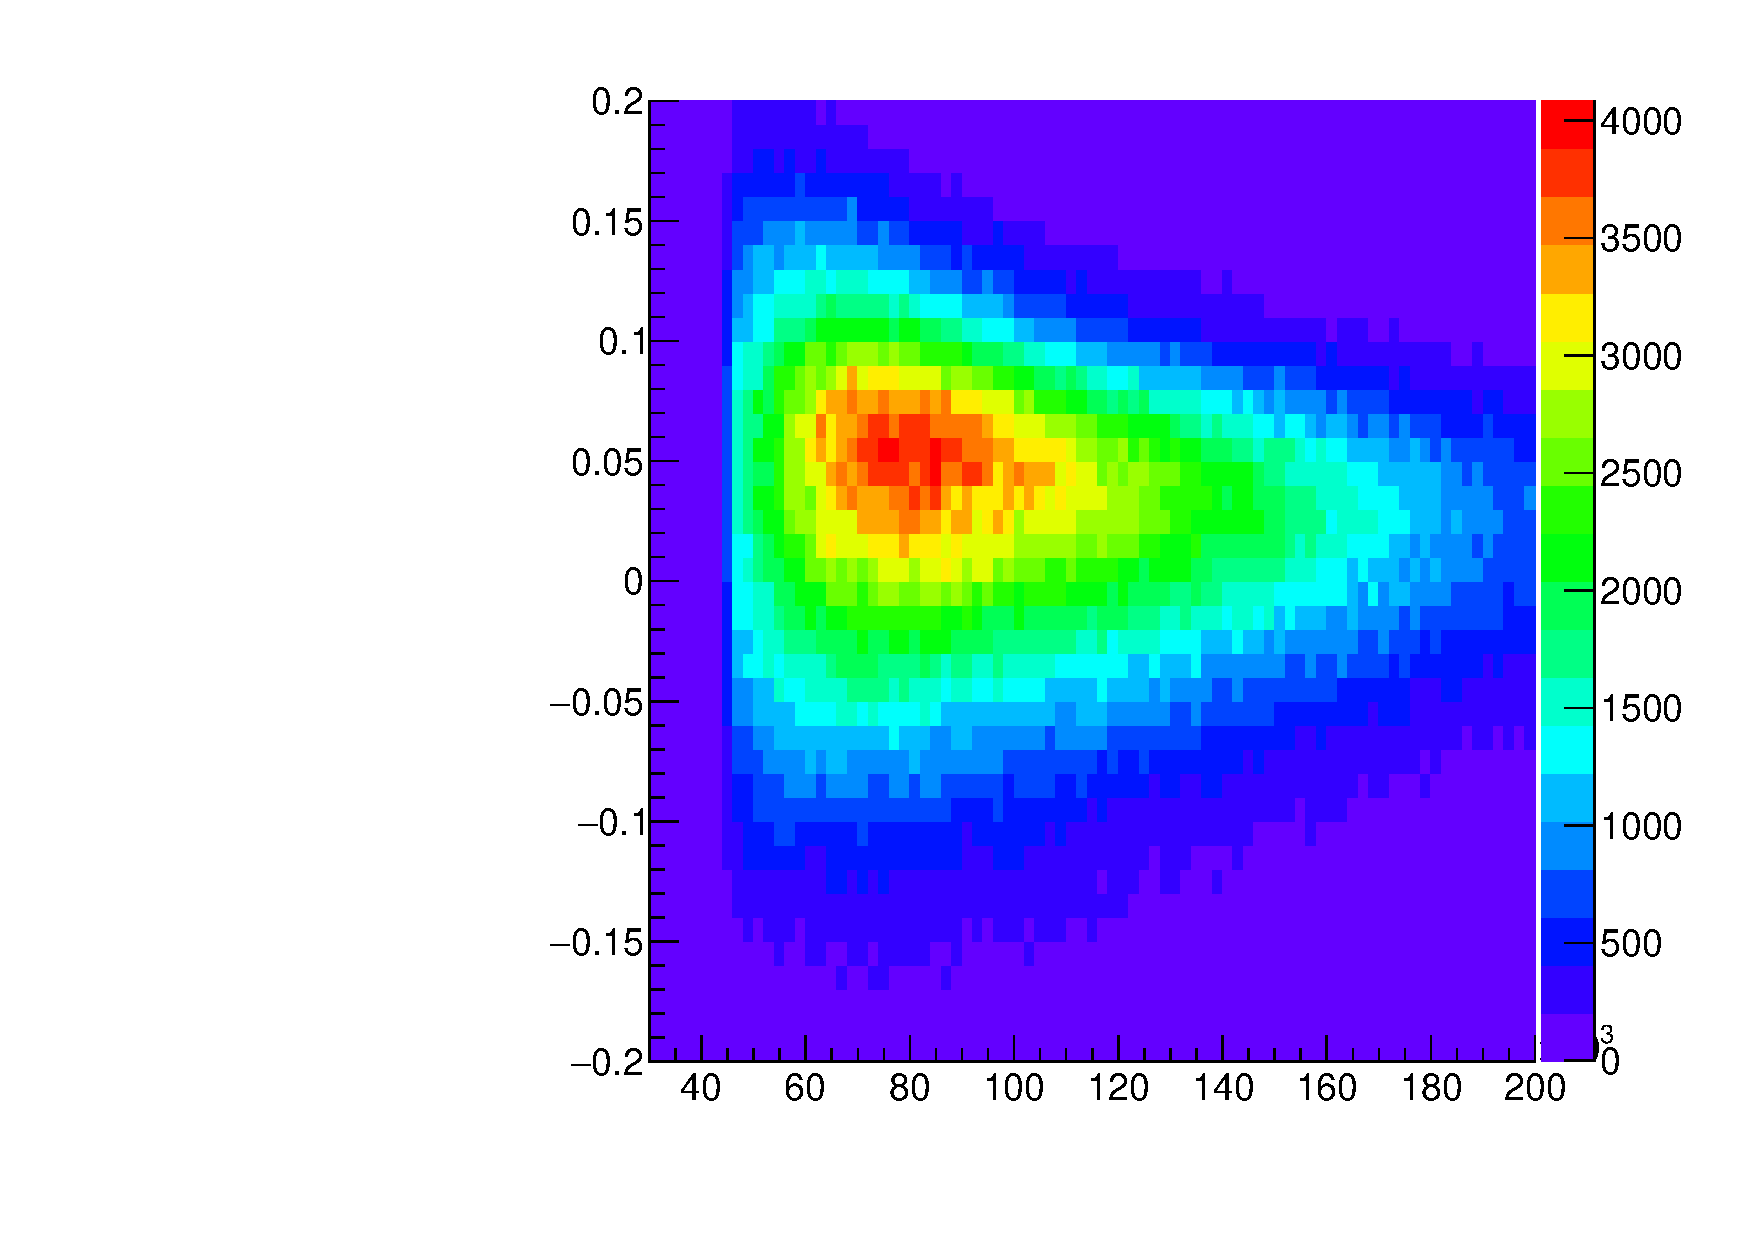
\includegraphics[width=1\linewidth]{ptRatio_Leading_Non_BJet}

			\end{minipage}
			\quad
			\begin{minipage}[h]{0.33\linewidth}
				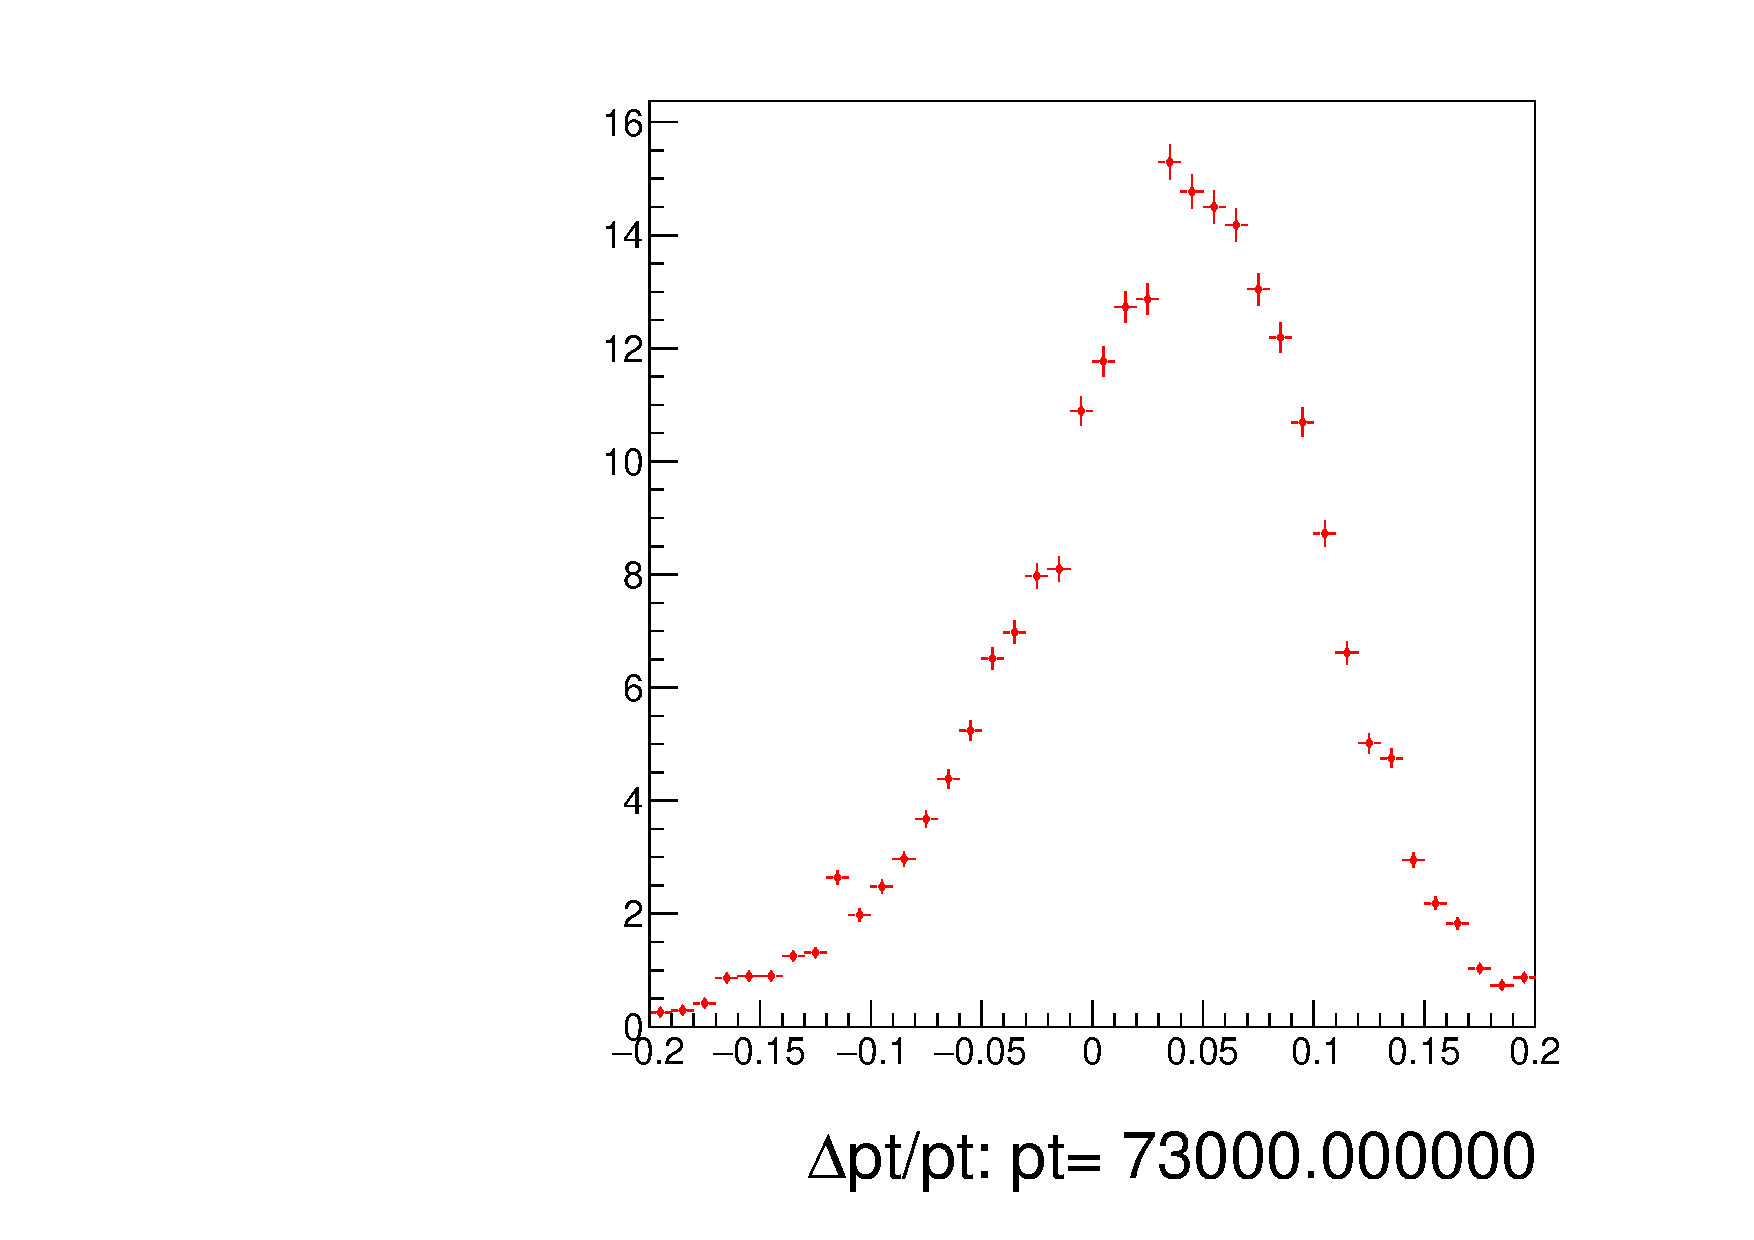
\includegraphics[width=1\linewidth]{ptRatio_Leading_Non_BJet_Slice}
			\end{minipage}
			\caption{$\Delta $\pt$_{ratio}$ for the leading \pt non $b$-jet from MC events against \pt of the offline $b$-jet. }
			\label{fig:MC:nonleadingbpt}
		\end{figure}

		\begin{figure}[h]
			\centering

			\begin{minipage}[h]{0.33\linewidth}
				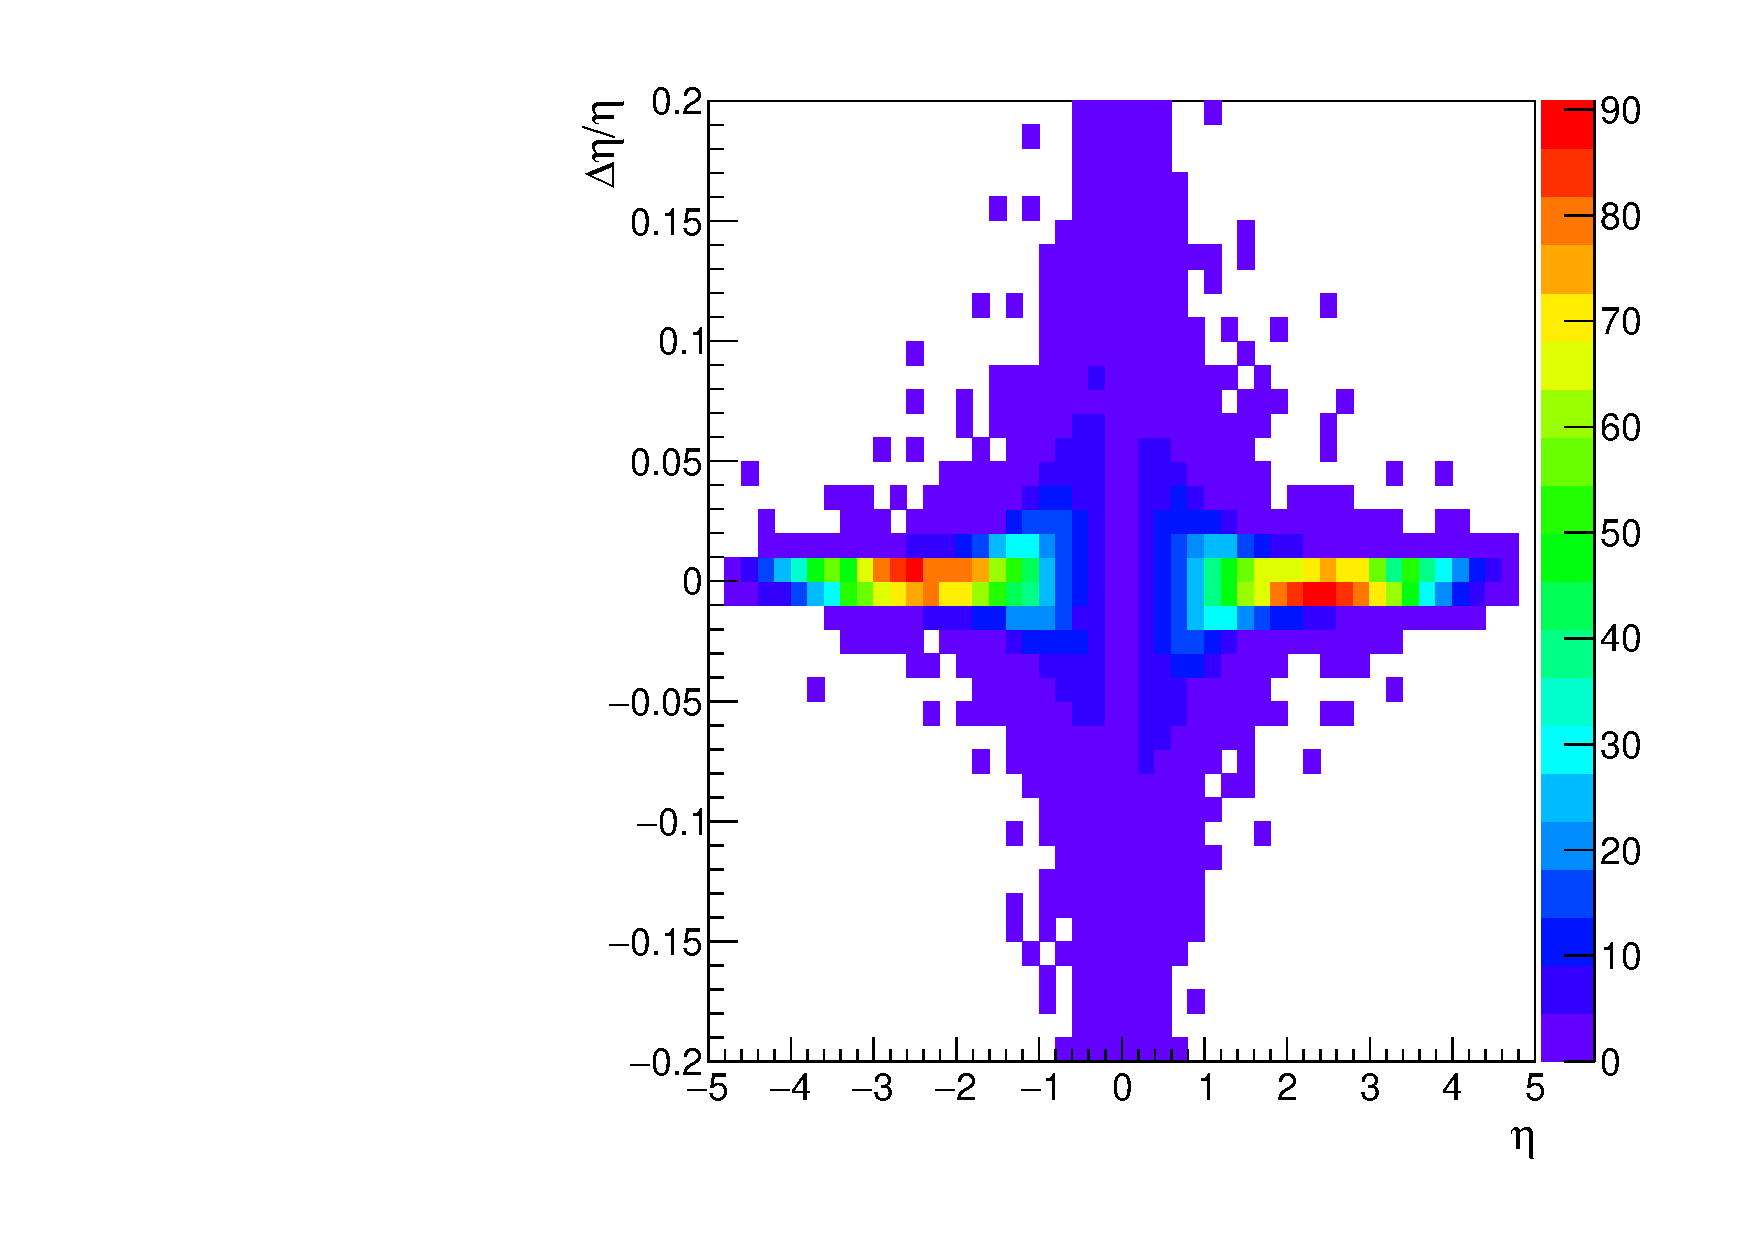
\includegraphics[width=1\linewidth]{etaRatio_Leading_Non_BJet}
			\end{minipage}
			\quad
			\begin{minipage}[h]{0.33\linewidth}
				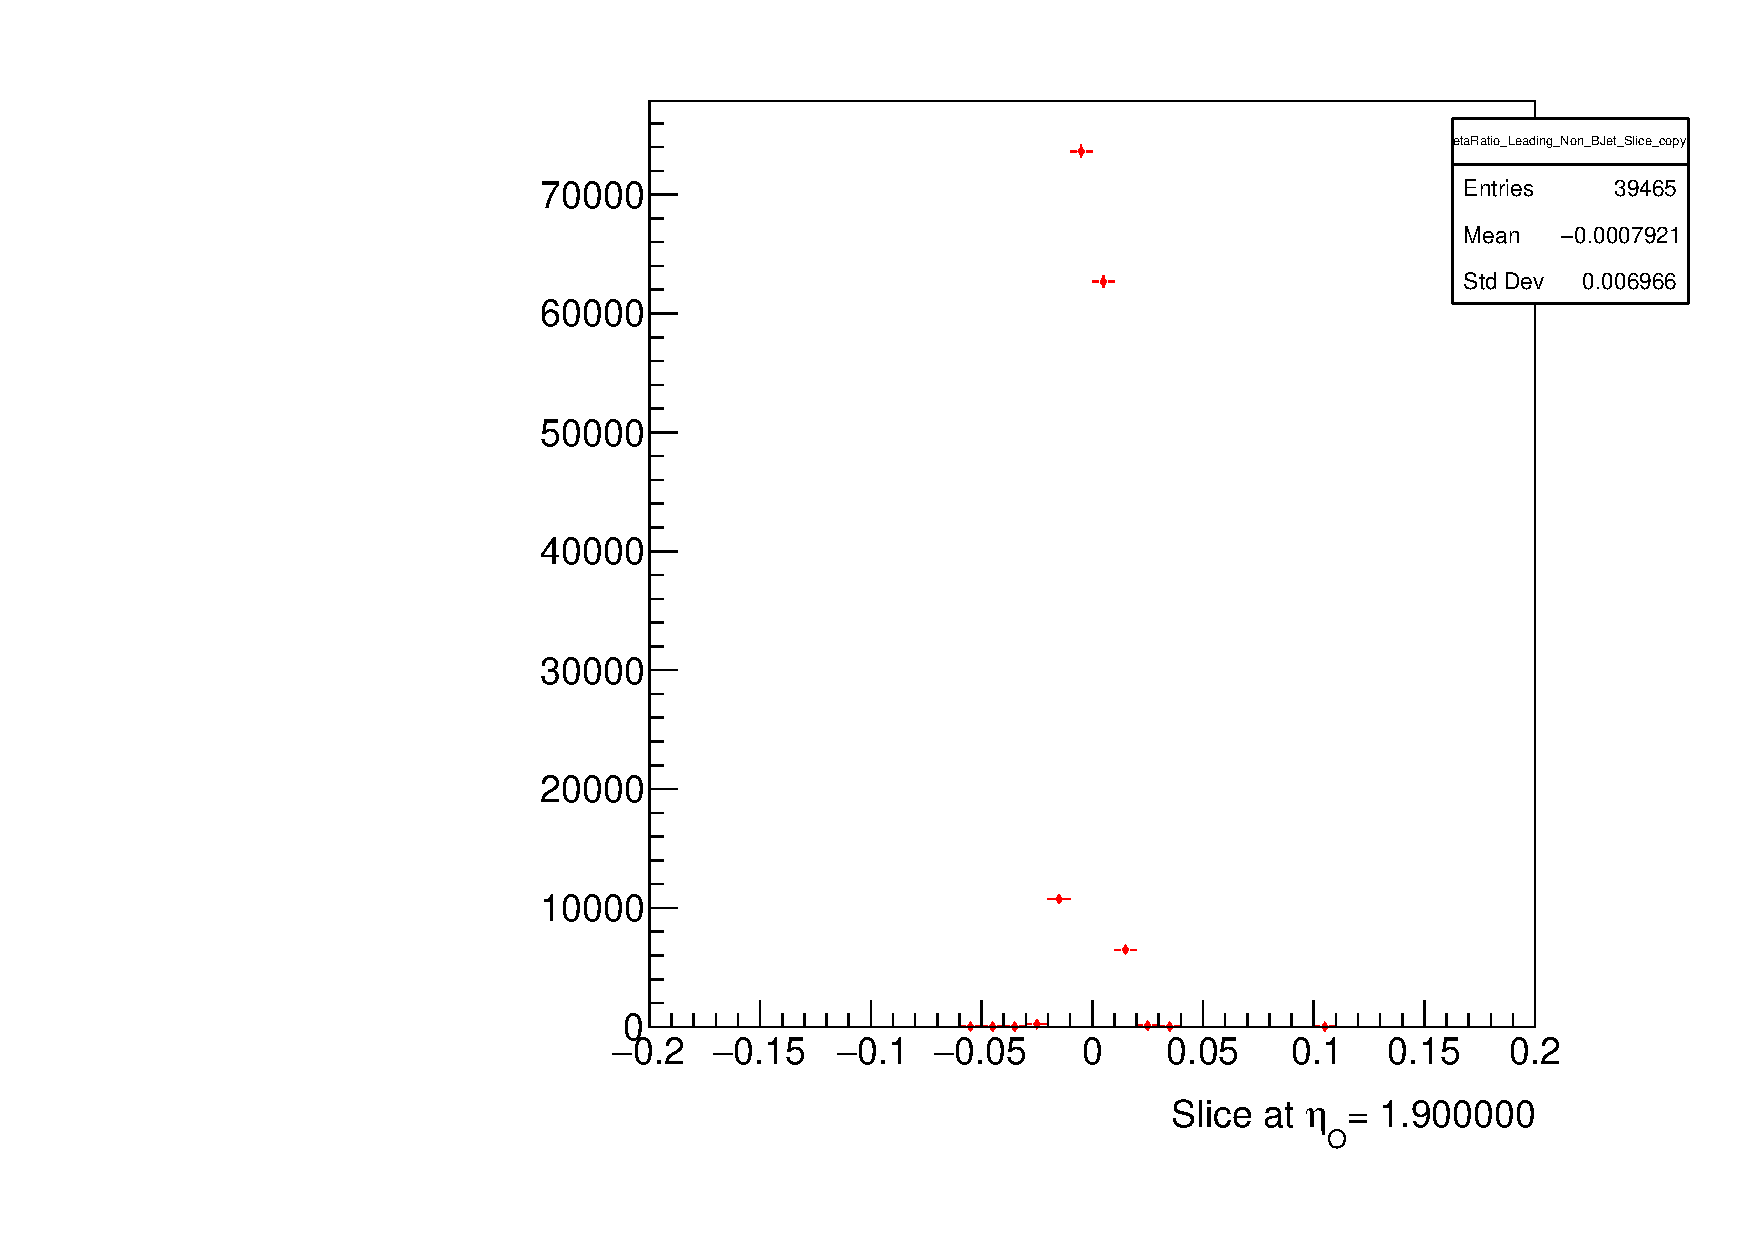
\includegraphics[width=1\linewidth]{etaRatio_Leading_Non_BJet_Slice}
			\end{minipage}
			\caption{$\Delta \eta_{ratio}$ for the leading \pt non $b$-jet from MC events against $\eta$ of the offline $b$-jet. }
			\label{fig:MC:nonleadingbeta}
		\end{figure}

		\begin{figure}[h]
			\centering

			\begin{minipage}[h]{0.33\linewidth}
				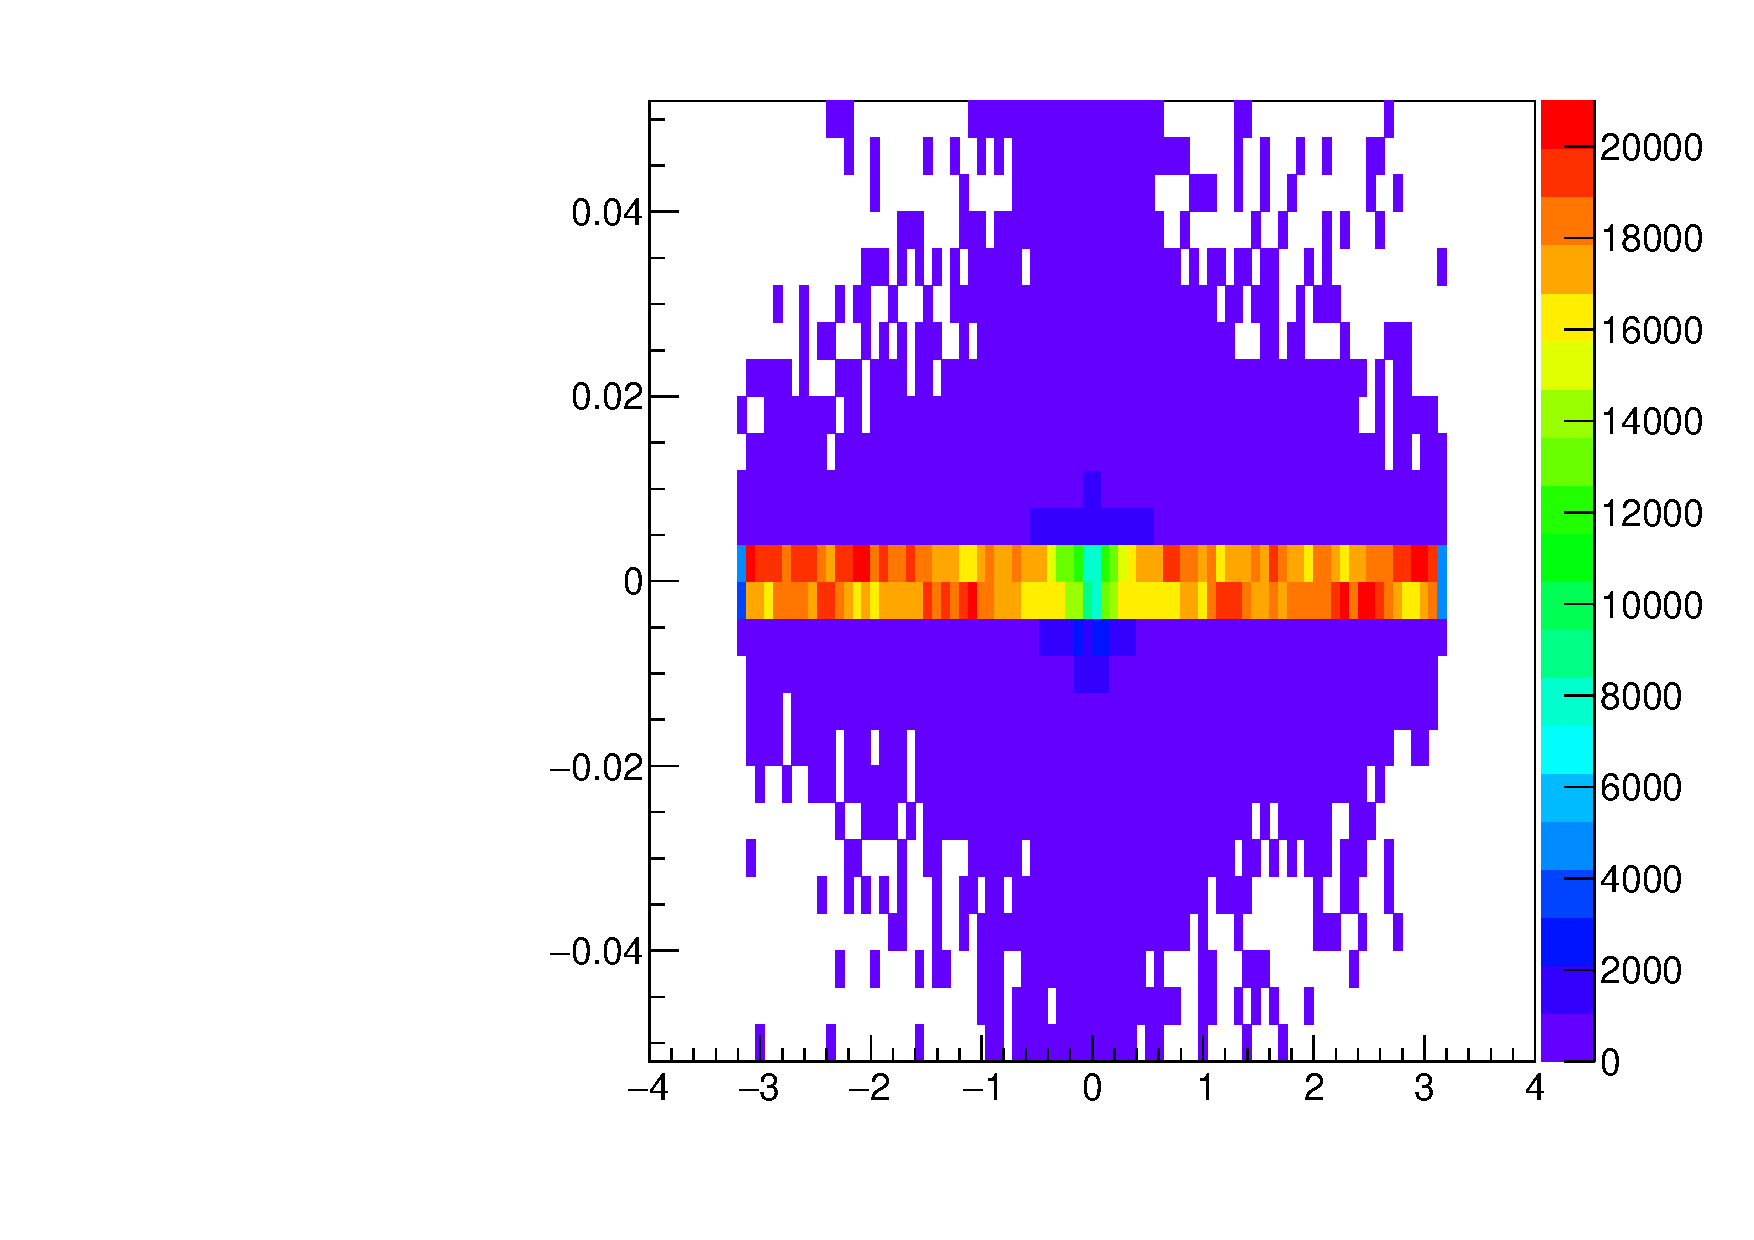
\includegraphics[width=1\linewidth]{phiRatio_Leading_Non_BJet}
			\end{minipage}
			\quad
			\begin{minipage}[h]{0.33\linewidth}
				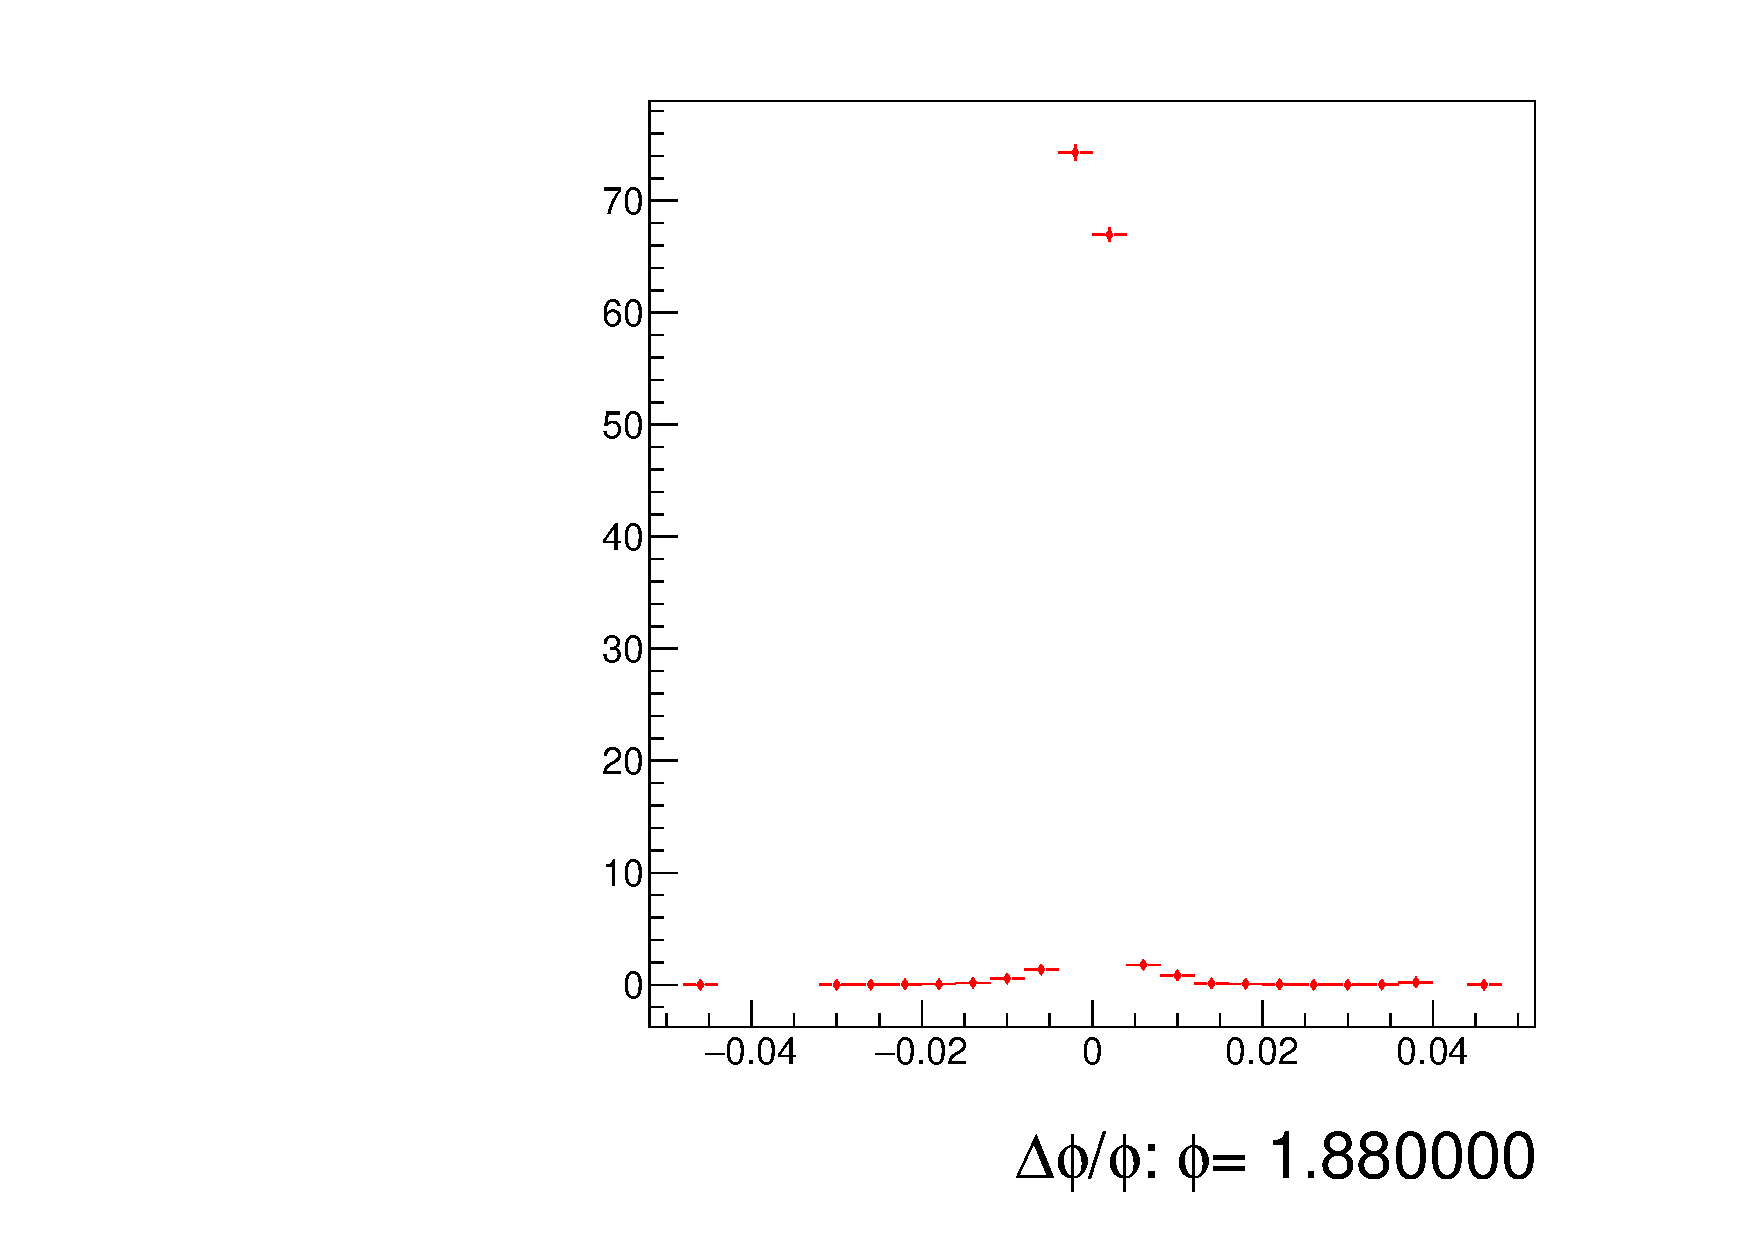
\includegraphics[width=1\linewidth]{phiRatio_Leading_Non_BJet_Slice}
			\end{minipage}
			\caption{$\Delta \phi_{ratio}$ for the leading \pt non $b$-jet from MC events against $\phi$ of the offline $b$-jet. }
			\label{fig:MC:nonleadingbphi}
		\end{figure}

		\begin{figure}[h]
			\centering

			\begin{minipage}[h]{0.33\linewidth}
				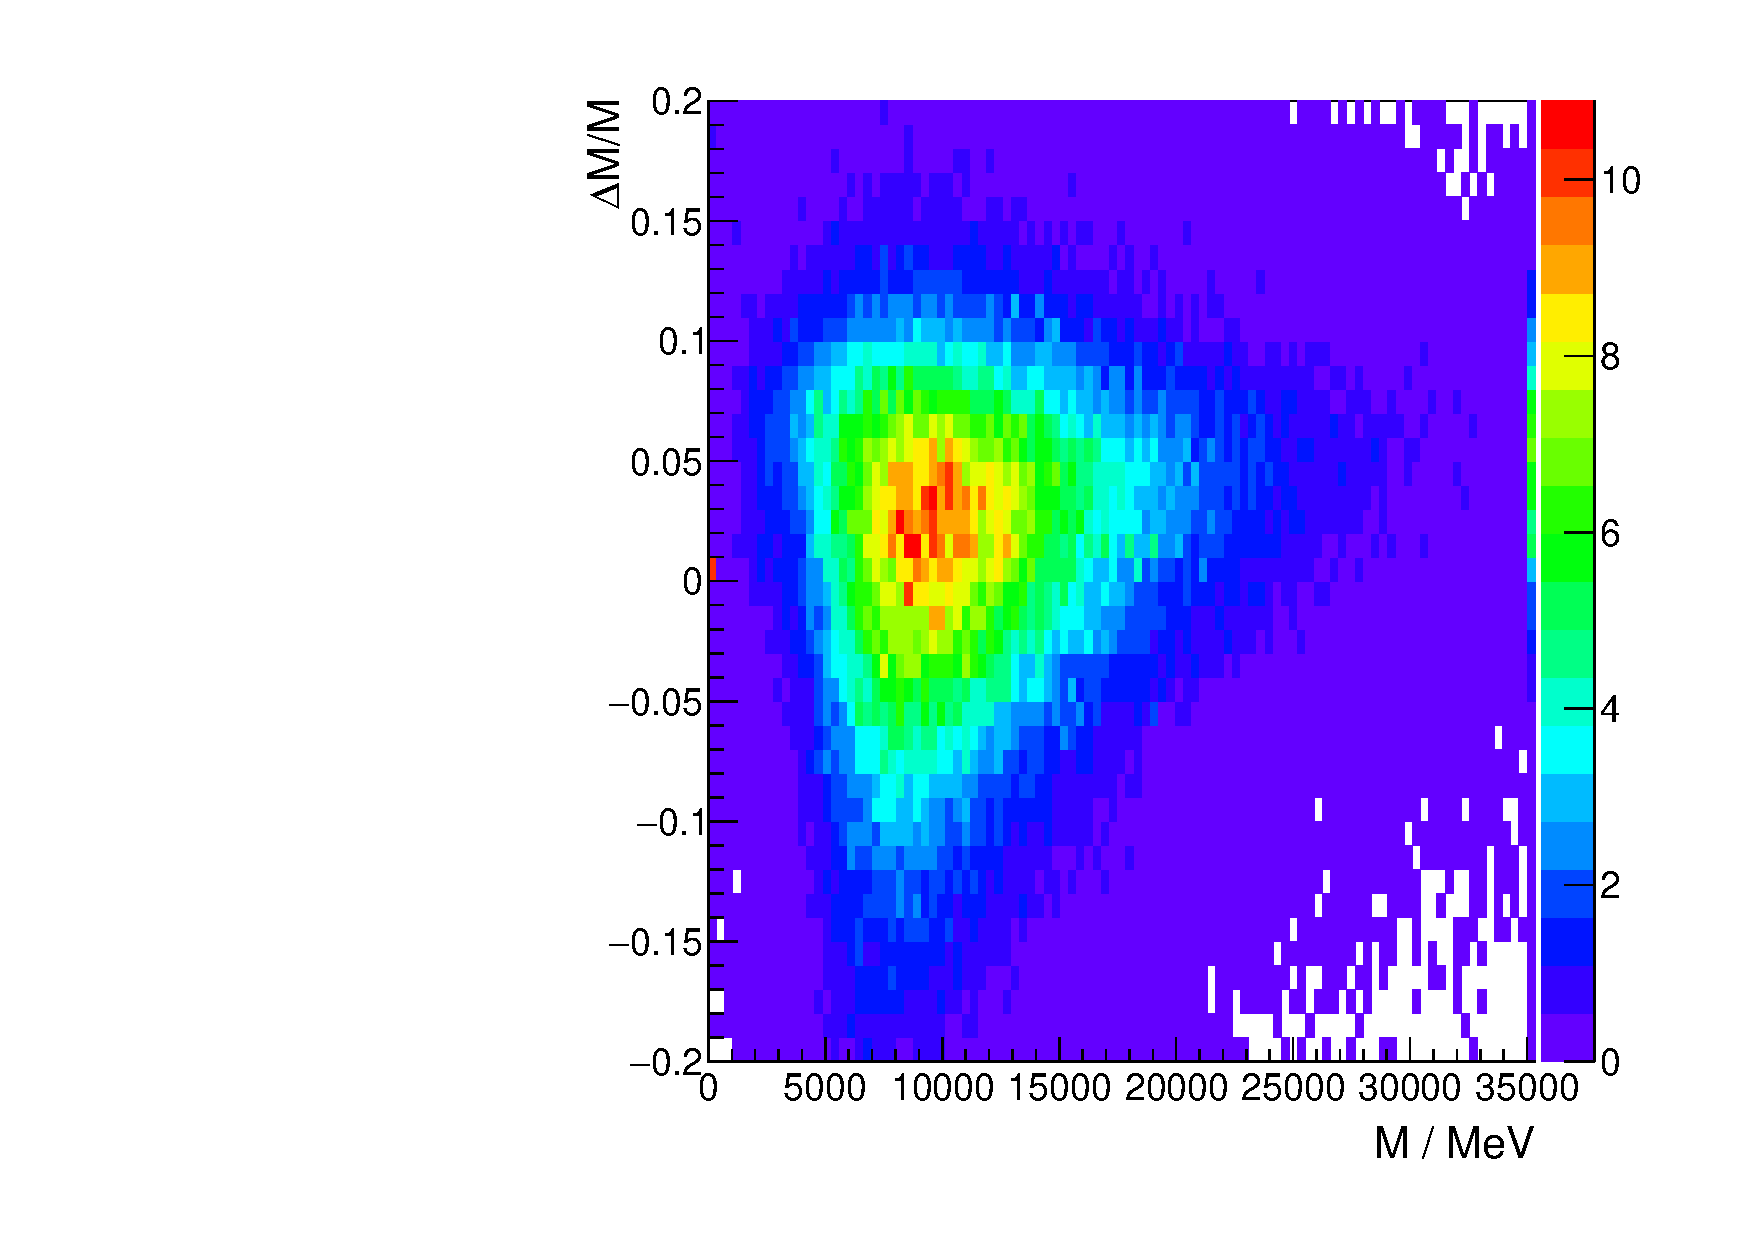
\includegraphics[width=1\linewidth]{mRatio_Leading_Non_BJet}
			\end{minipage}
			\quad
			\begin{minipage}[h]{0.33\linewidth}
				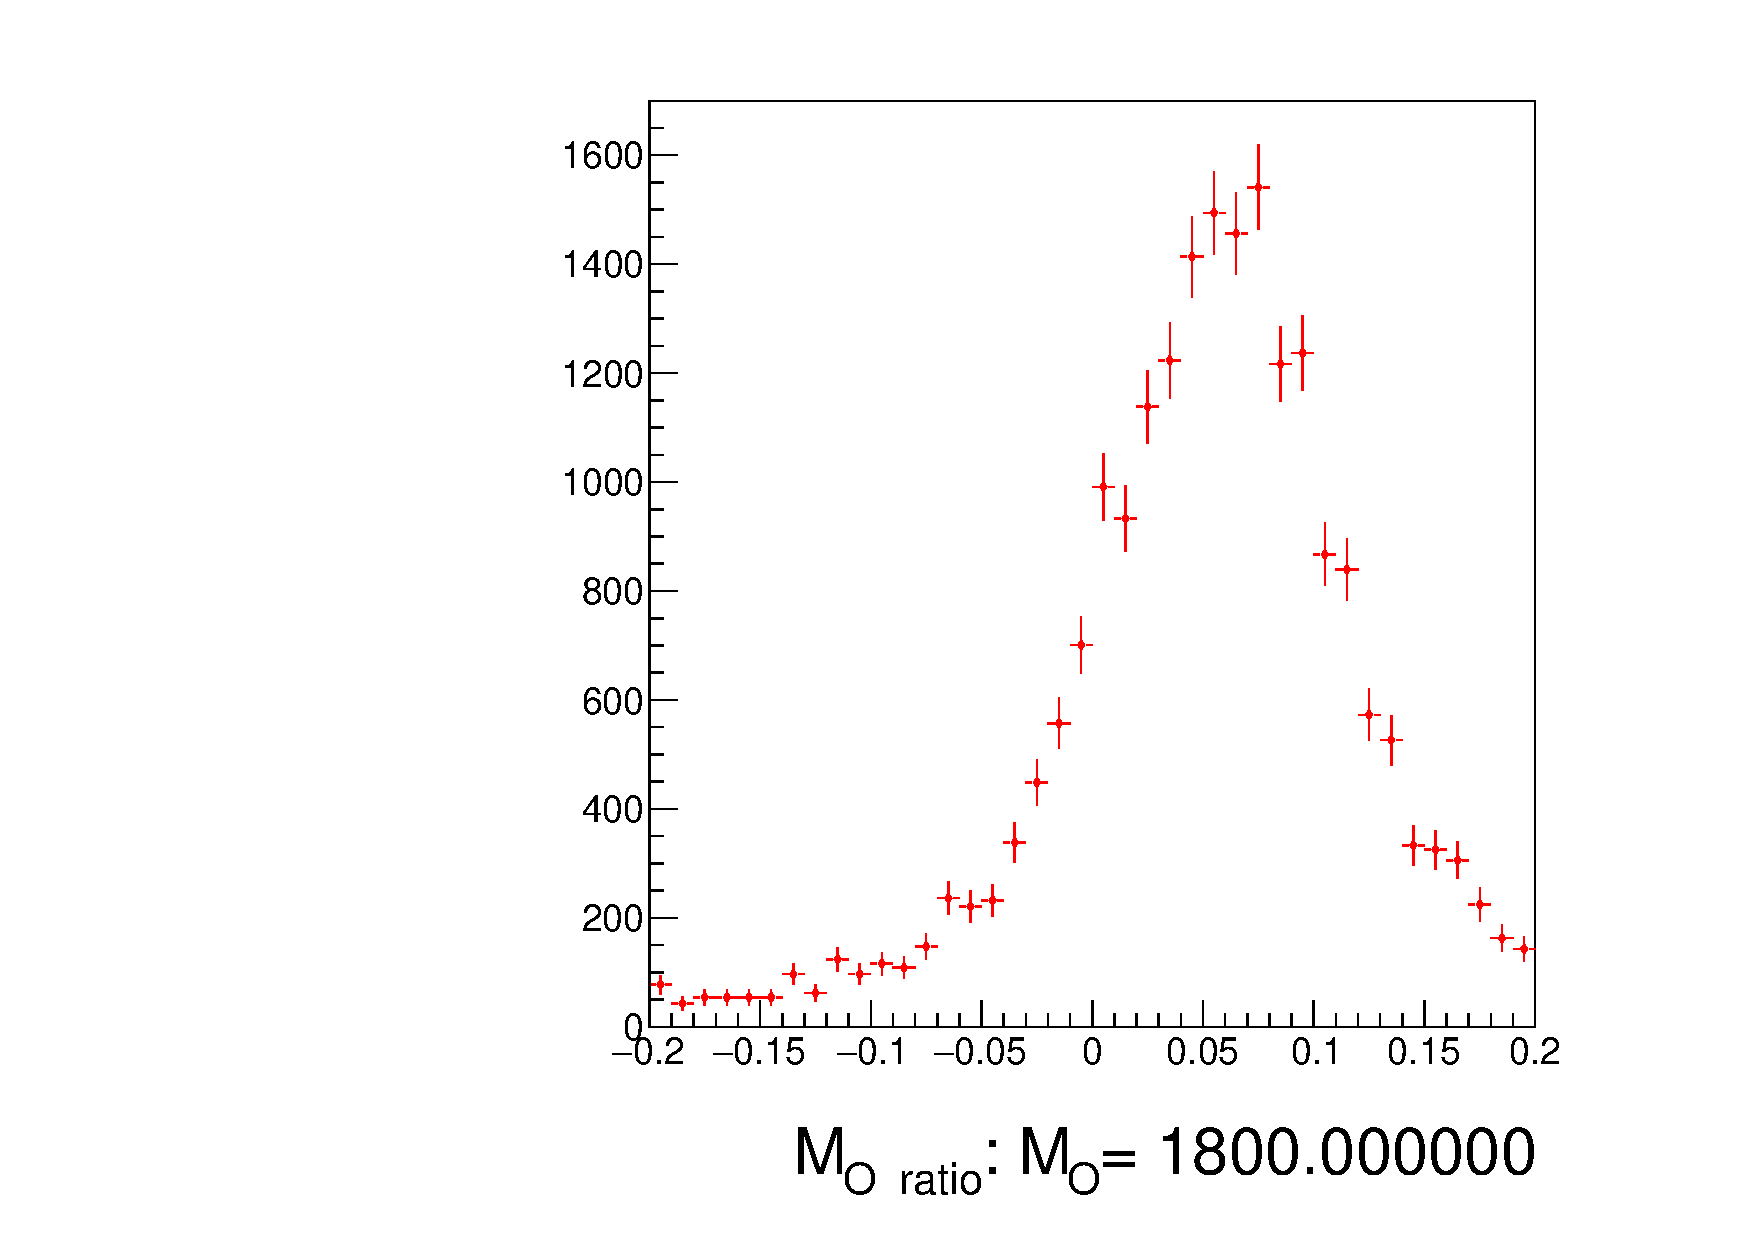
\includegraphics[width=1\linewidth]{mRatio_Leading_Non_BJet_Slice}
			\end{minipage}
			\caption{$\Delta M_{ratio}$ for the leading \pt non $b$-jet from MC events against $M$ of the offline $b$-jet. }
			\label{fig:MC:nonleadingbm}
		\end{figure}

	\newpage
	\subsection{Data}
	
	

		\begin{figure}[h]
			\centering
			\begin{minipage}[h]{0.33\linewidth}
				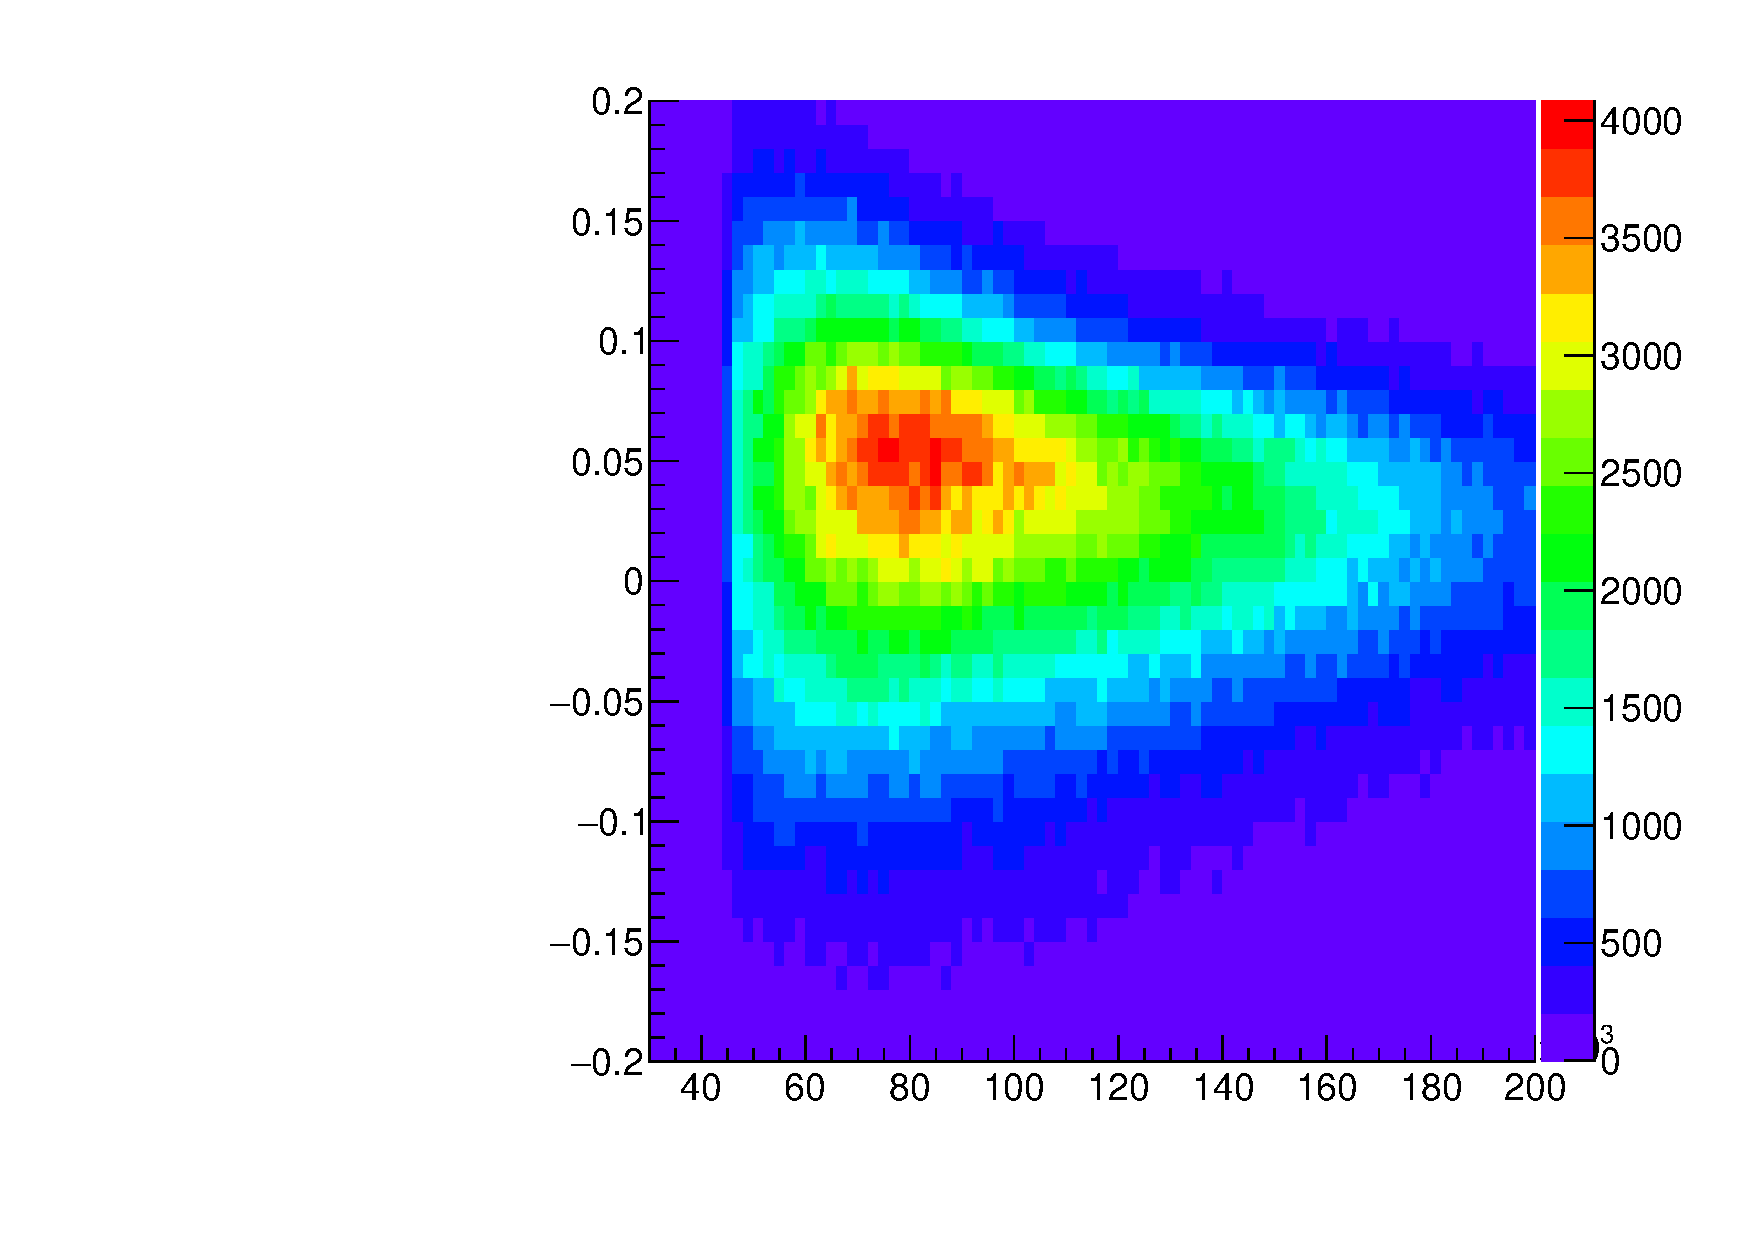
\includegraphics[width=1\linewidth]{ptRatio_Leading_Non_BJet}
				
			\end{minipage}
			\quad
			\begin{minipage}[h]{0.33\linewidth}
				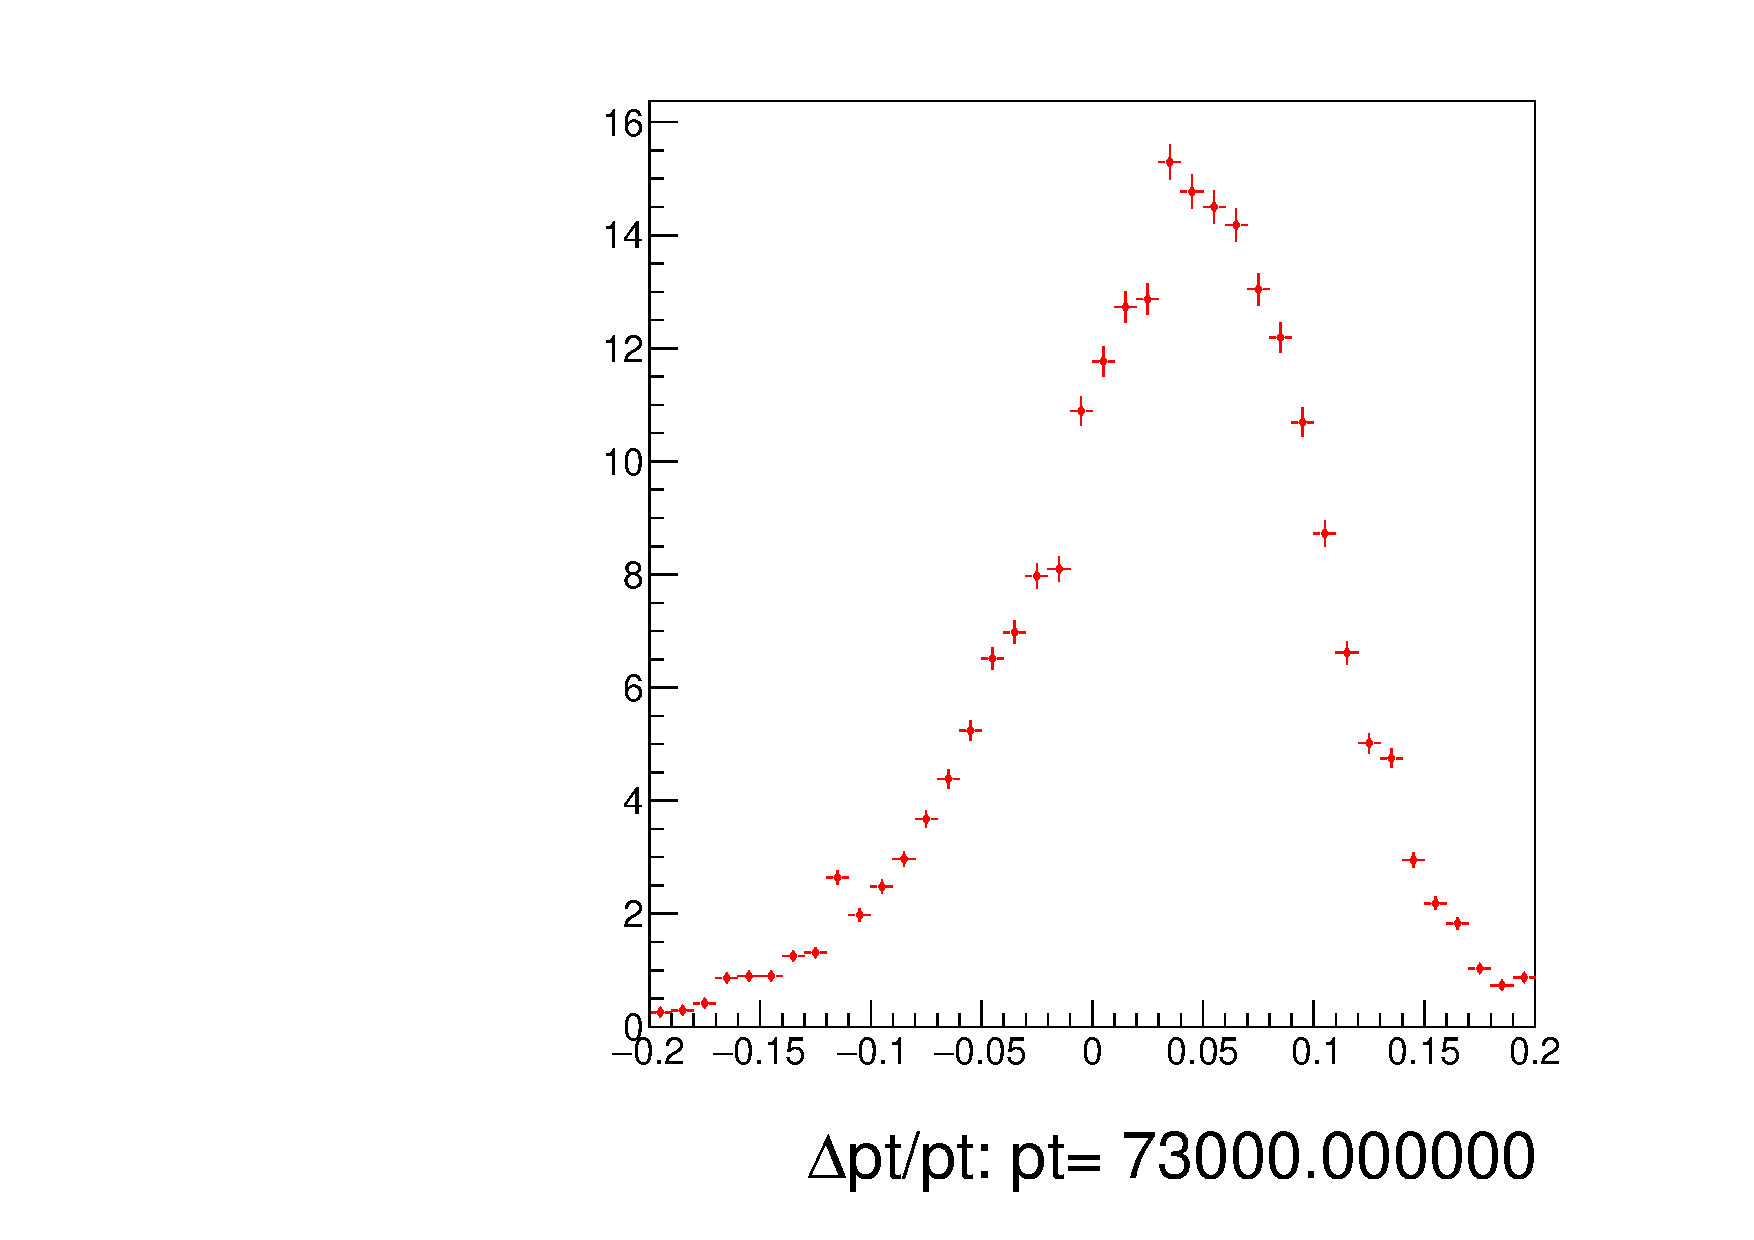
\includegraphics[width=1\linewidth]{ptRatio_Leading_Non_BJet_Slice}
			\end{minipage}
			\caption{$\Delta $\pt$_{ratio}$ for the leading \pt non $b$-jet from Data events against \pt of the offline $b$-jet. }
			\label{fig:D:nonleadingbpt}
		\end{figure}
		
		\begin{figure}[h]
			\centering
			
			\begin{minipage}[h]{0.33\linewidth}
				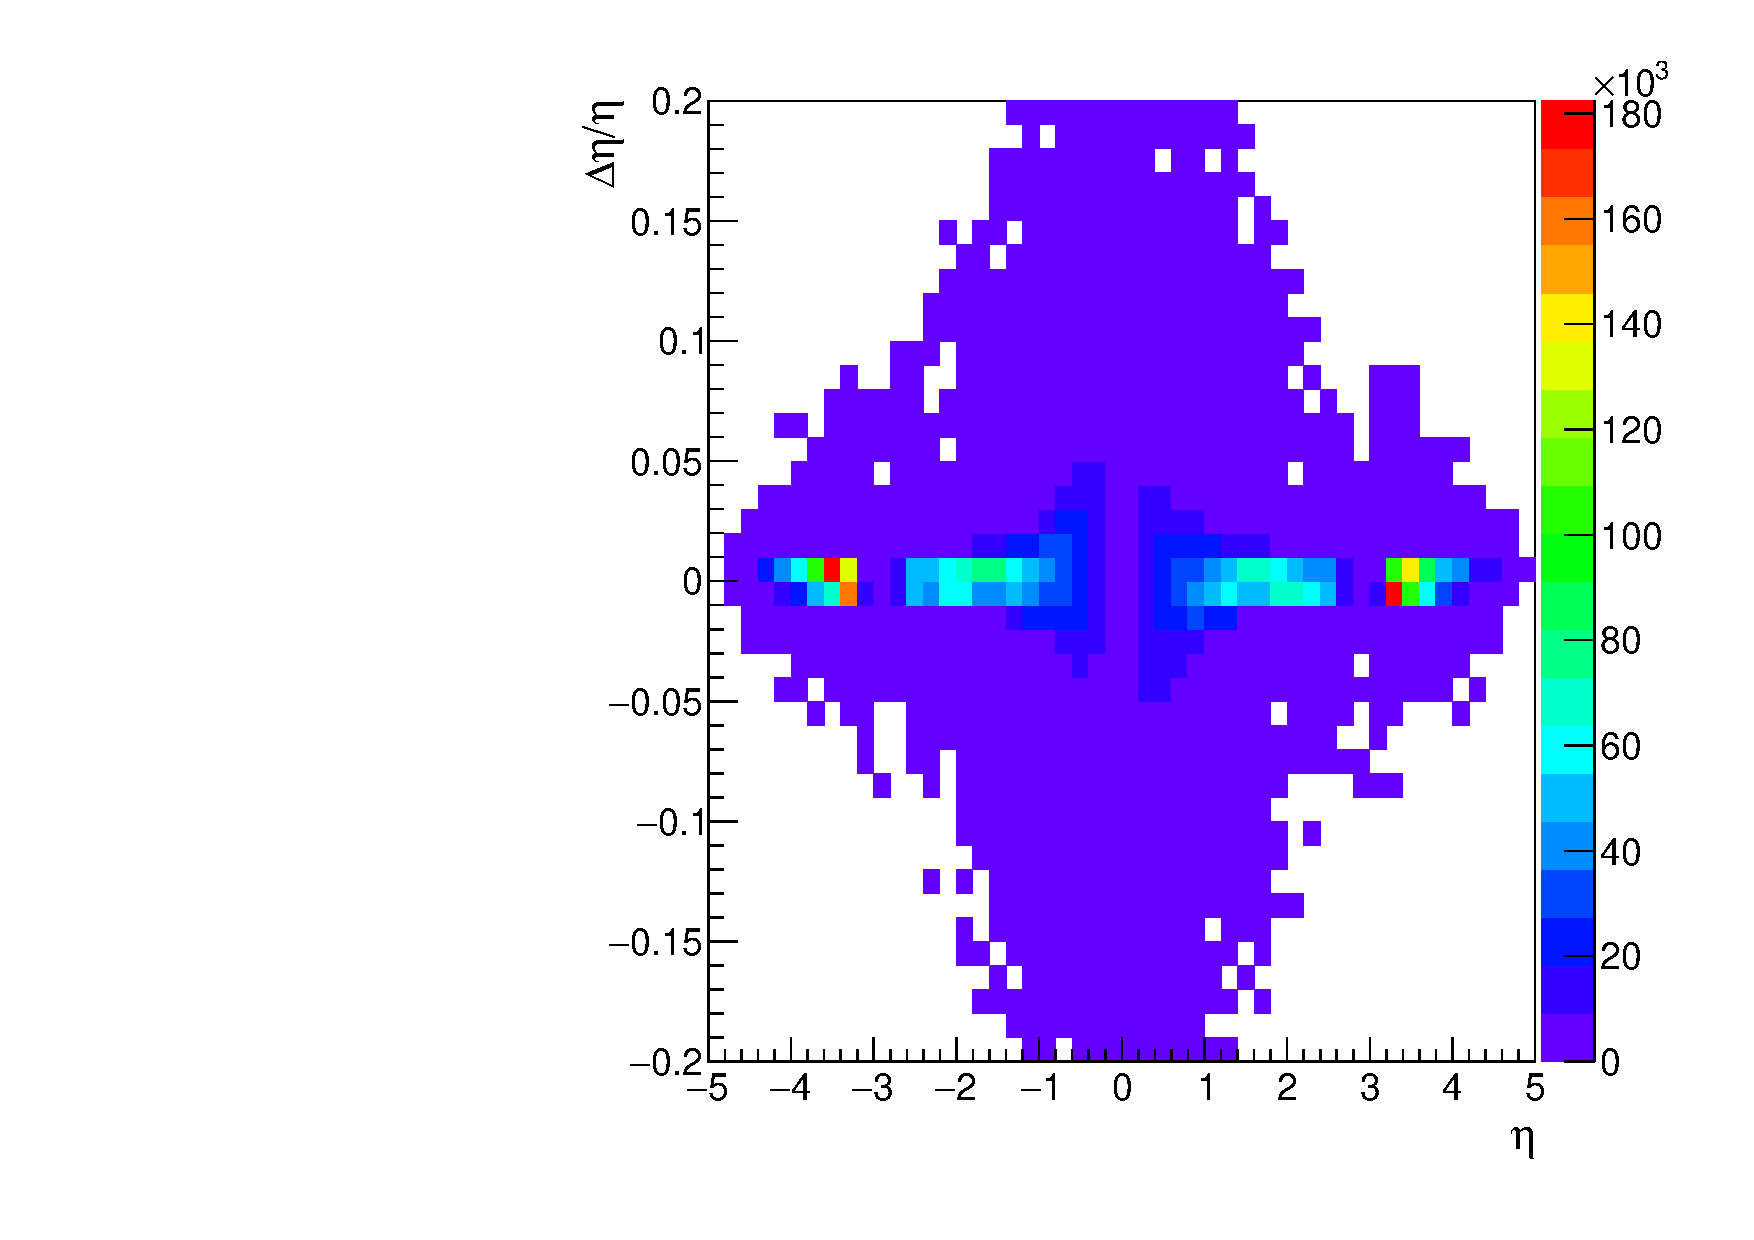
\includegraphics[width=1\linewidth]{Offline_2C_etaRatio_Leading_Non_BJet}
			\end{minipage}
			\quad
			\begin{minipage}[h]{0.33\linewidth}
				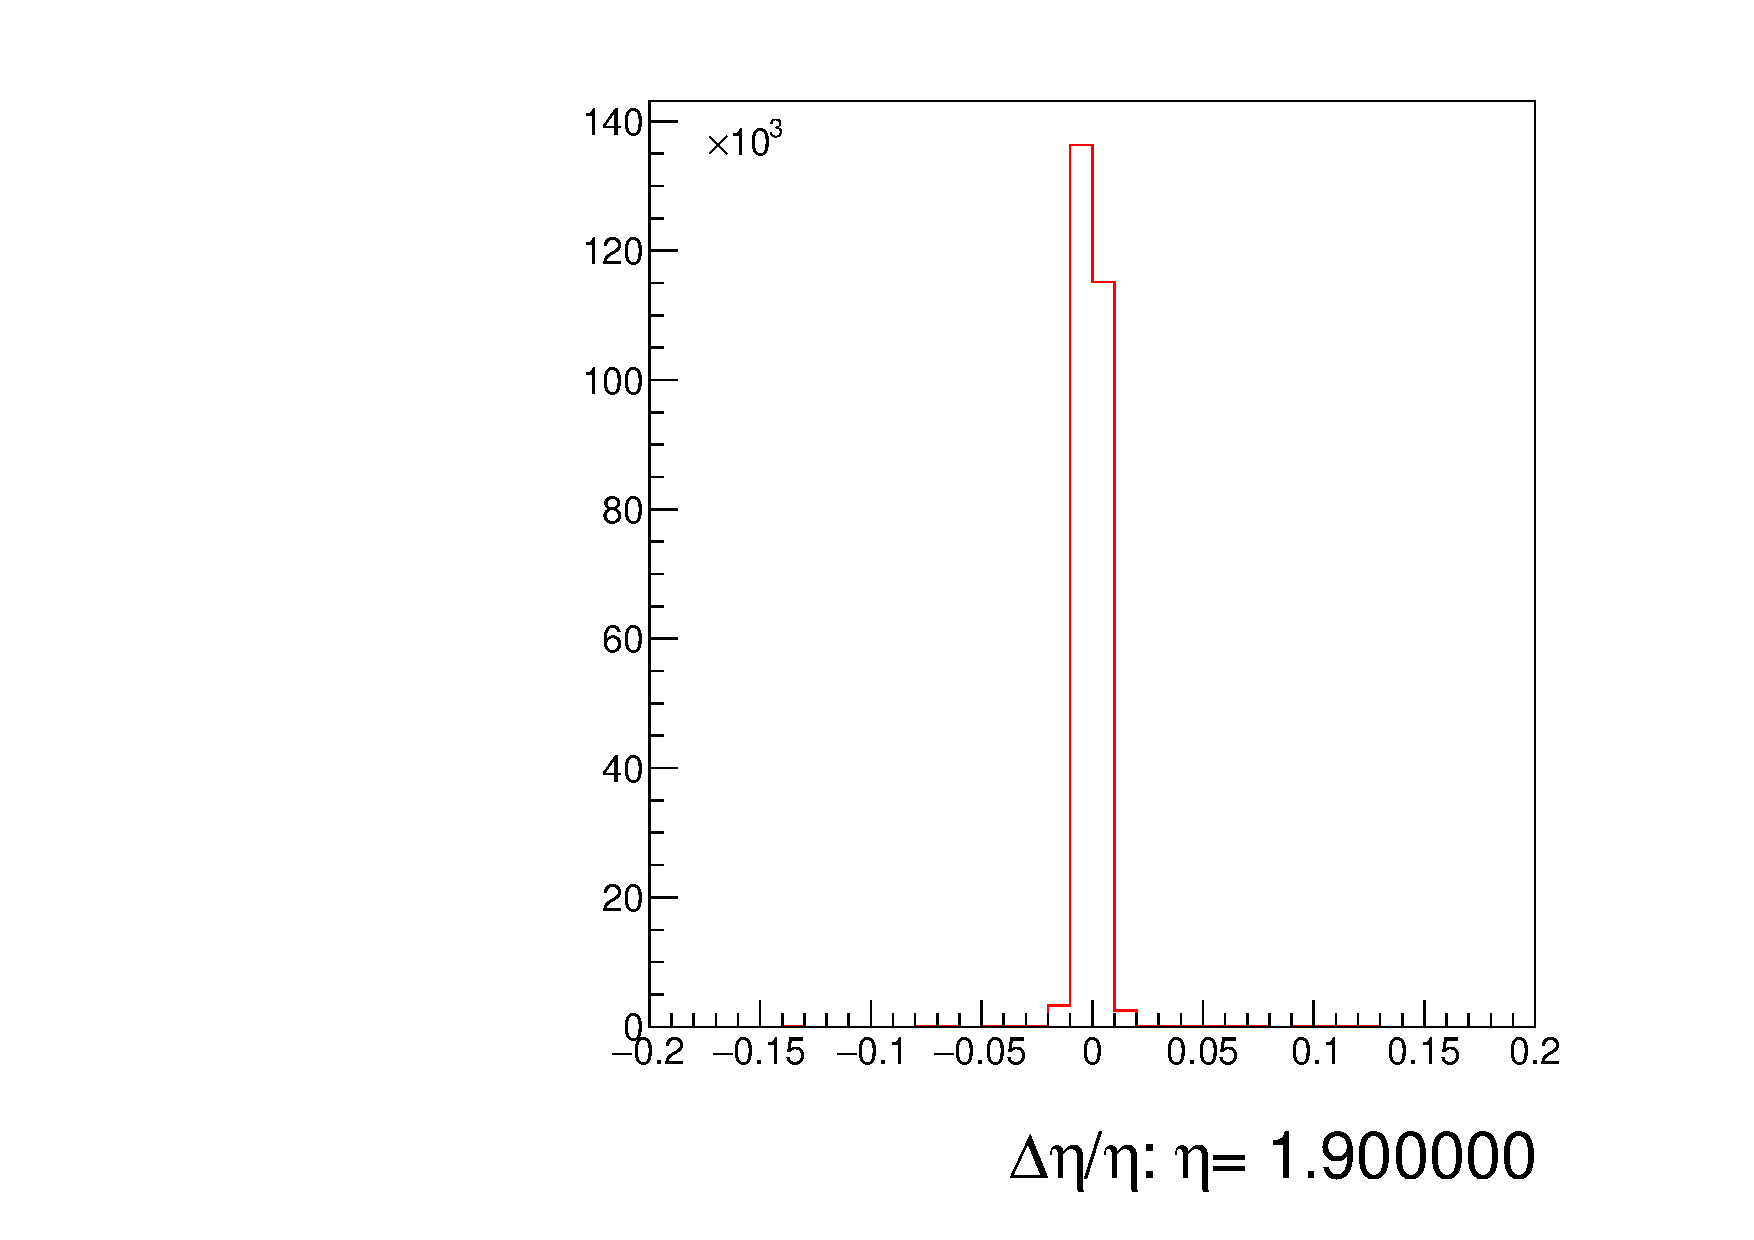
\includegraphics[width=1\linewidth]{Offline_2C_etaRatio_Leading_Non_BJet_Slice}
			\end{minipage}
			\caption{$\Delta \eta_{ratio}$ for the leading \pt non $b$-jet from Data events against $\eta$ of the offline $b$-jet. }
			\label{fig:D:nonleadingbeta}
		\end{figure}
		
		\begin{figure}[h]
			\centering
			
			\begin{minipage}[h]{0.33\linewidth}
				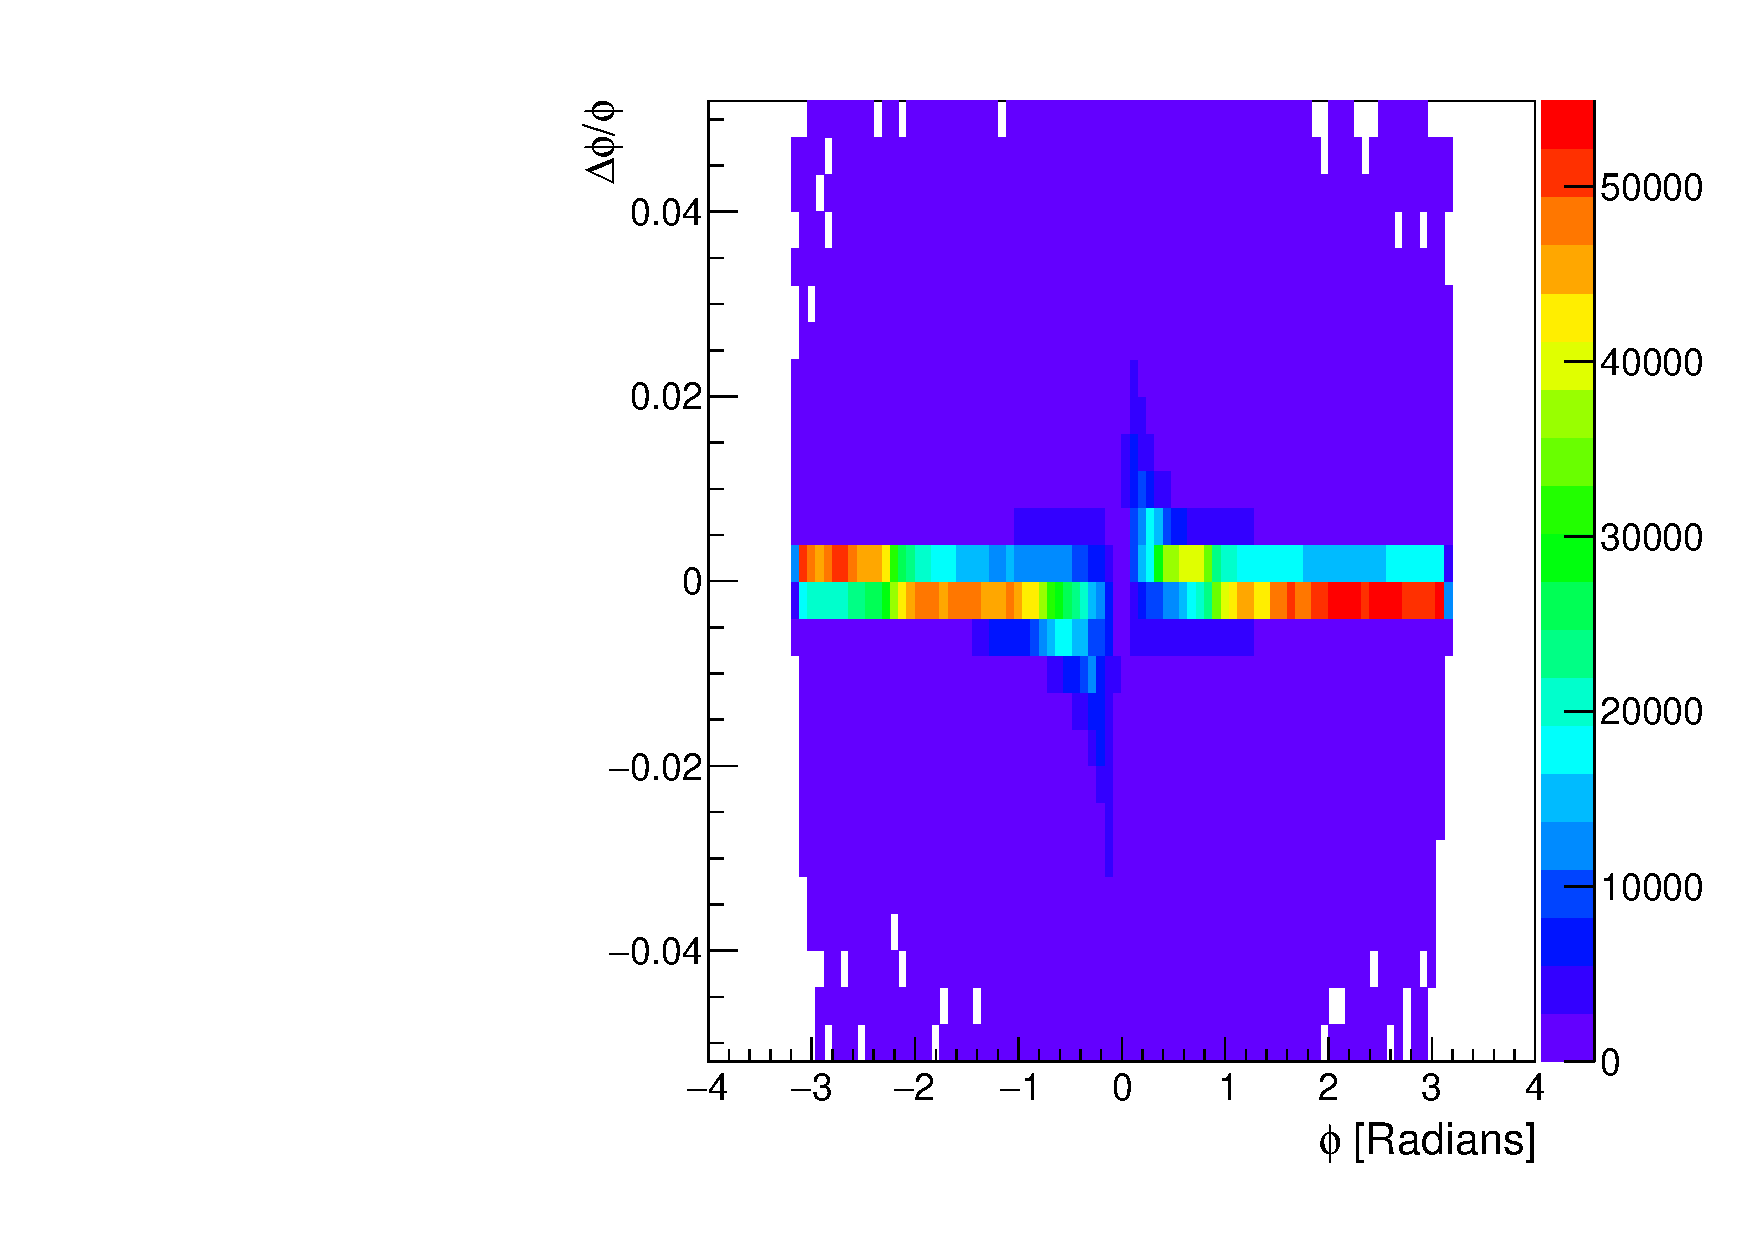
\includegraphics[width=1\linewidth]{Offline_2C_phiRatio_Leading_Non_BJet}
			\end{minipage}
			\quad
			\begin{minipage}[h]{0.33\linewidth}
				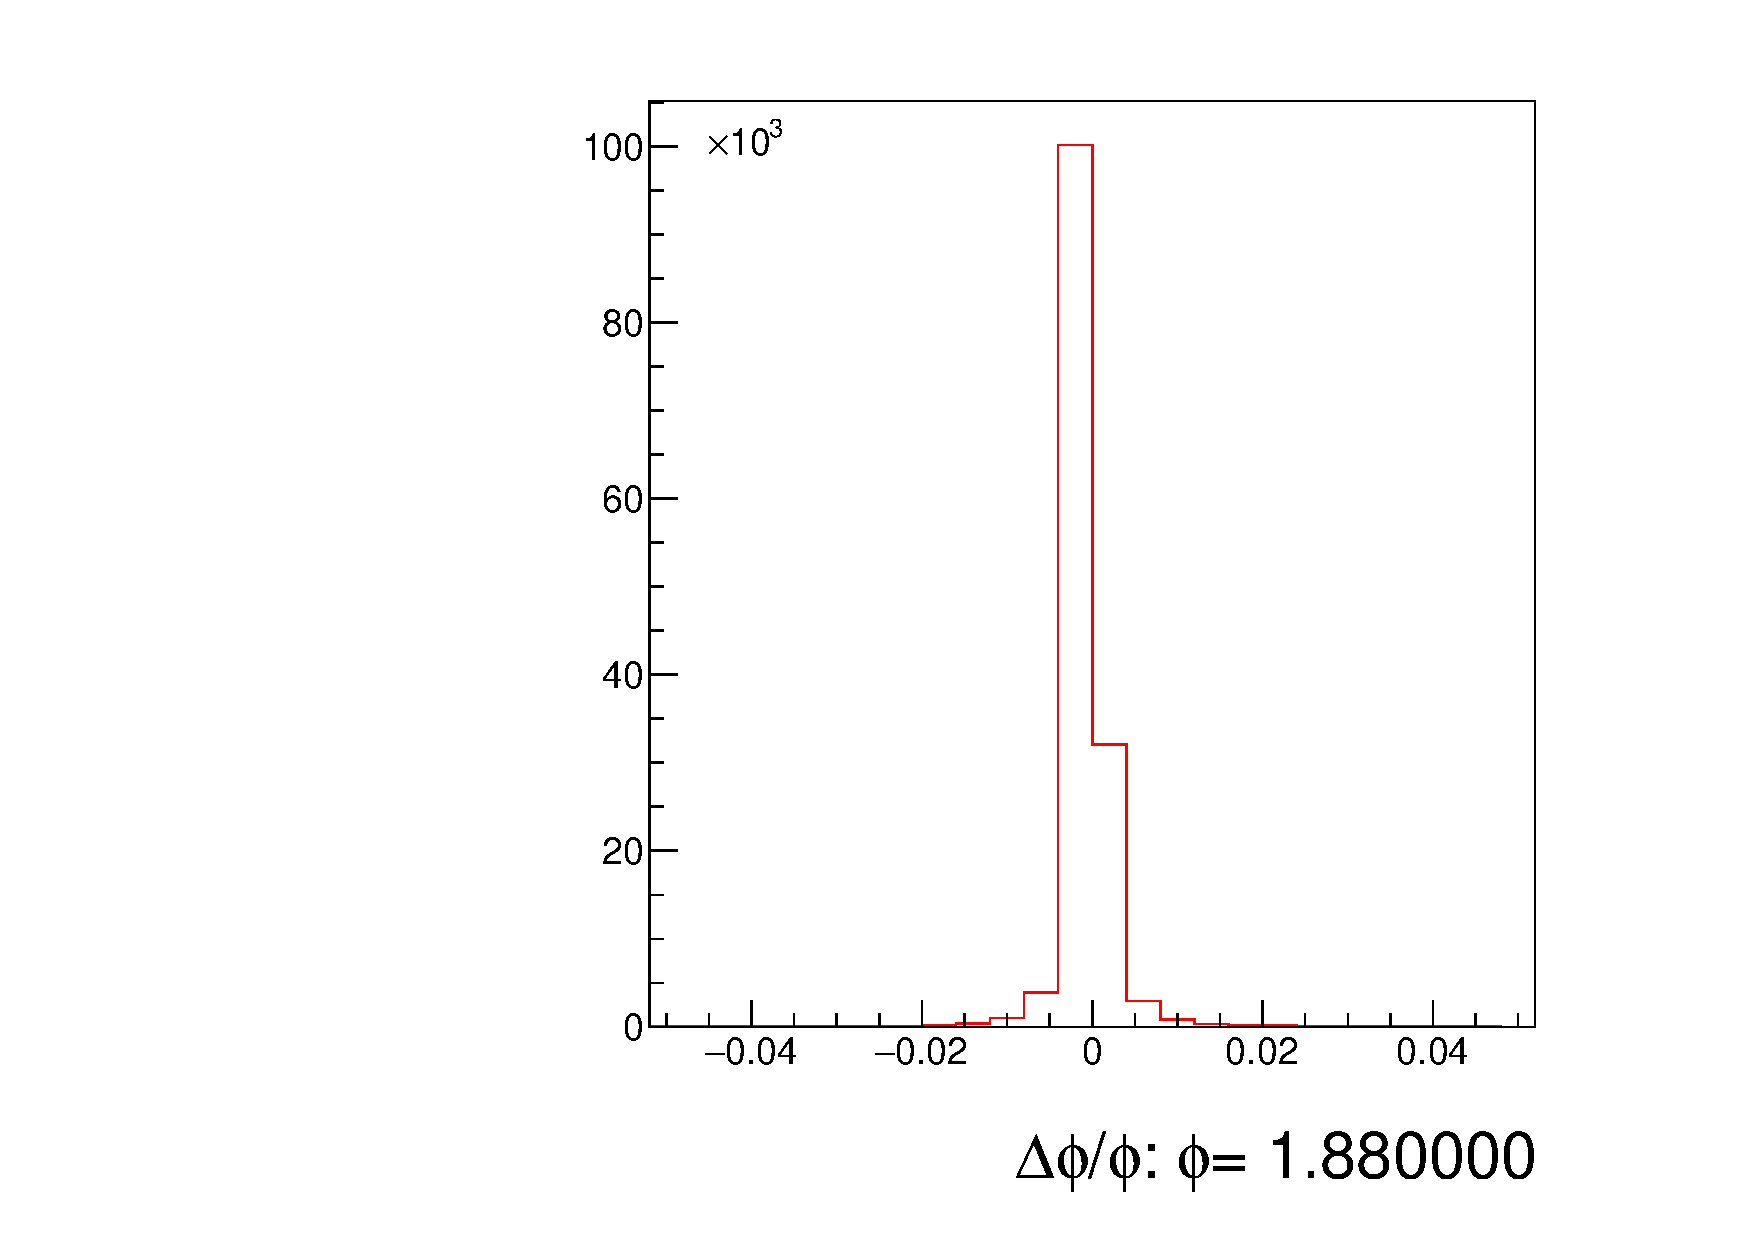
\includegraphics[width=1\linewidth]{Offline_2C_phiRatio_Leading_Non_BJet_Slice}
			\end{minipage}
			\caption{$\Delta \phi_{ratio}$ for the leading \pt non $b$-jet from Data events against $\phi$ of the offline $b$-jet. }
			\label{fig:D:nonleadingbphi}
		\end{figure}
		
		\begin{figure}[htb]
			\centering
			
			\begin{minipage}[h]{0.33\linewidth}
				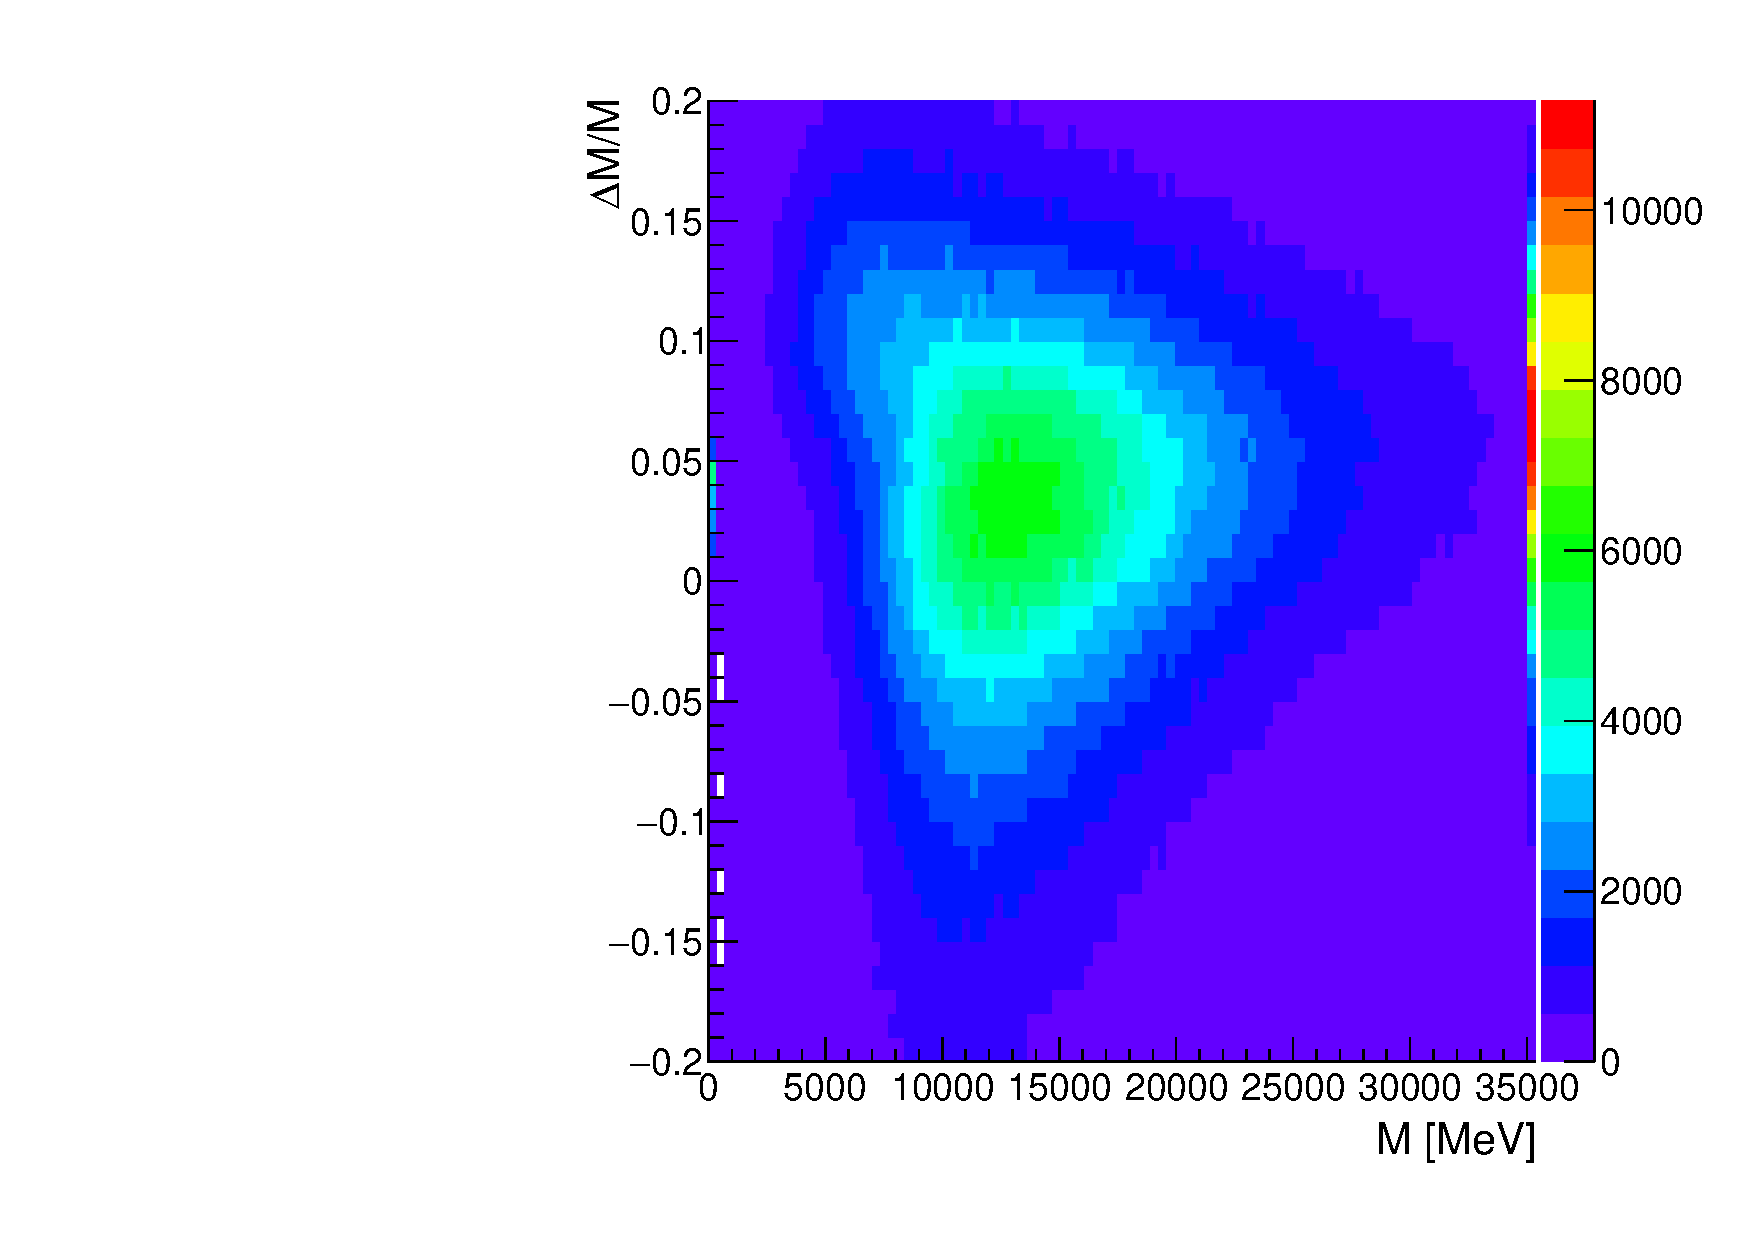
\includegraphics[width=1\linewidth]{Offline_2C_mRatio_Leading_Non_BJet}
			\end{minipage}
			\quad
			\begin{minipage}[h]{0.33\linewidth}
				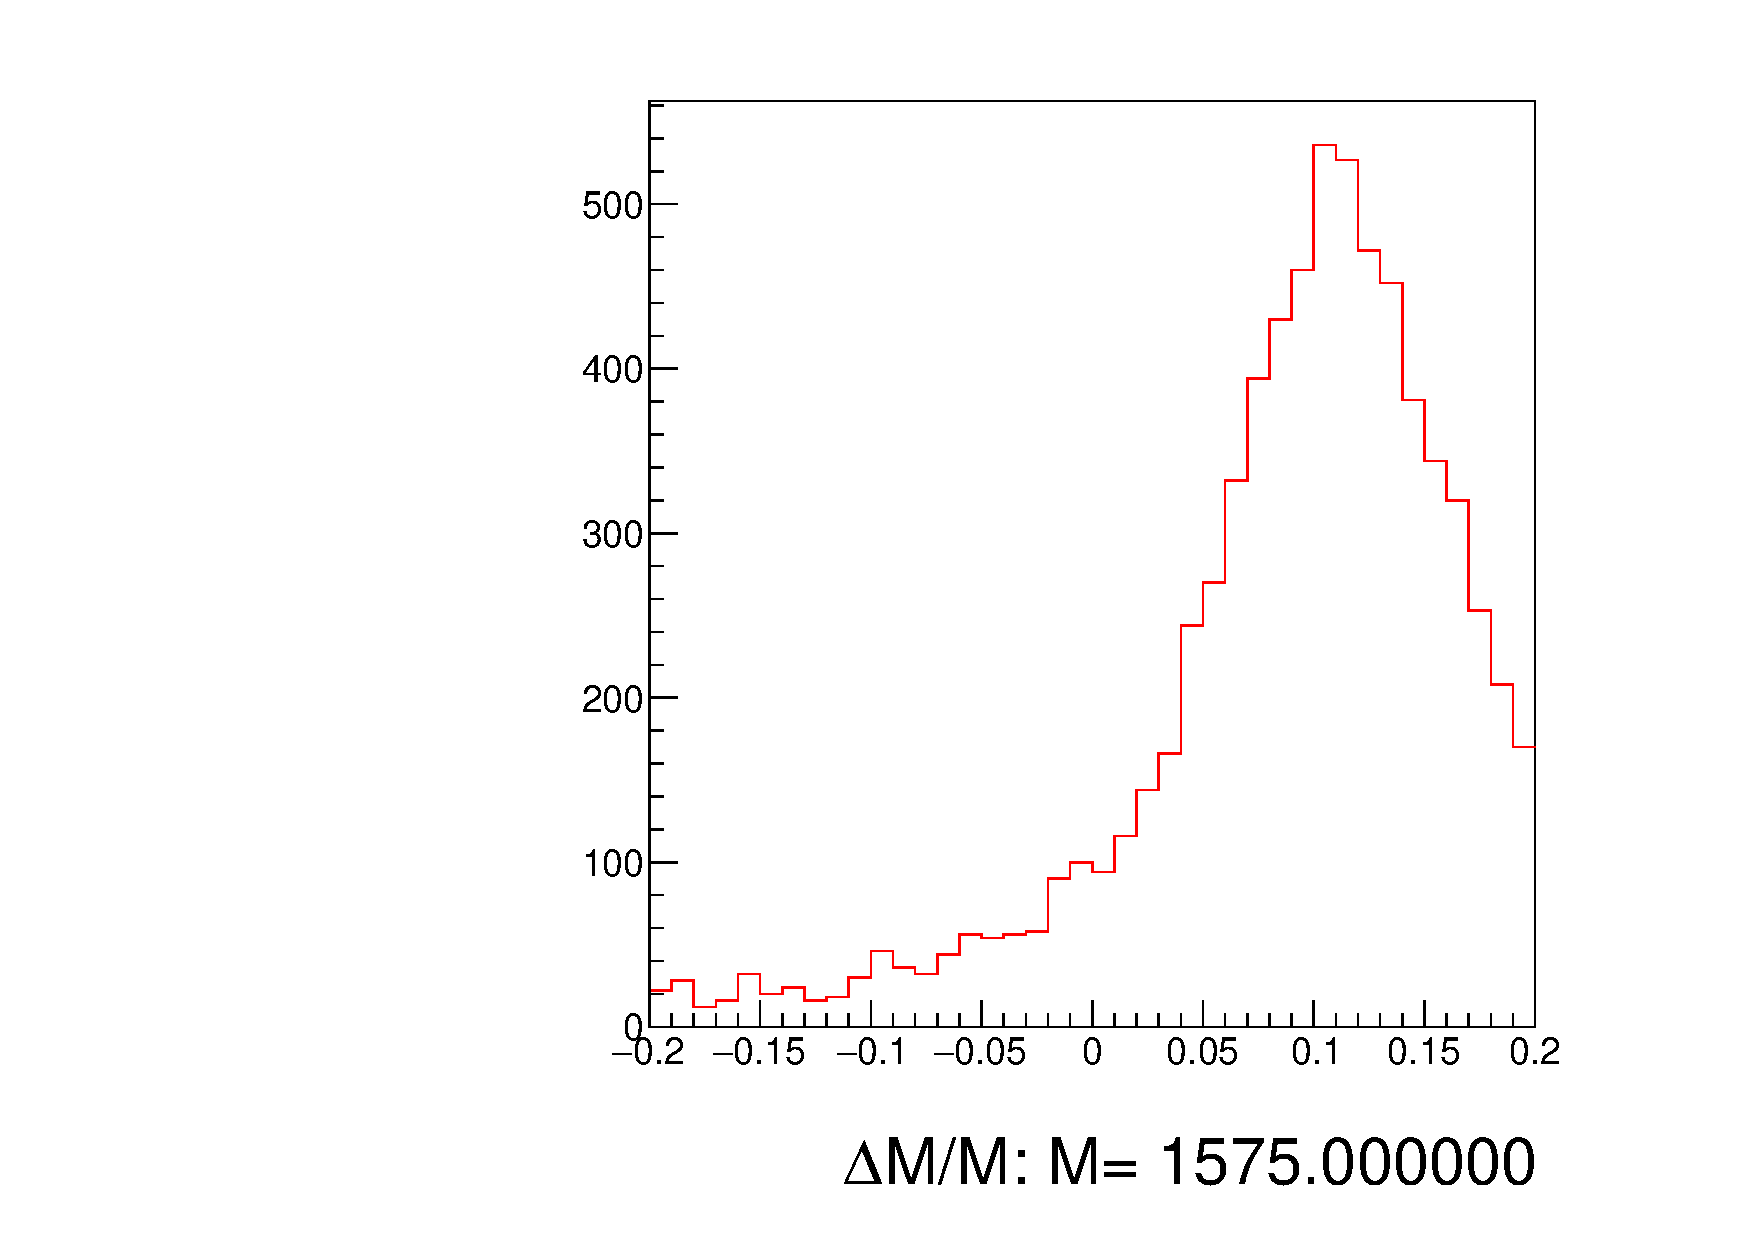
\includegraphics[width=1\linewidth]{Offline_2C_mRatio_Leading_Non_BJet_Slice}
			\end{minipage}
			\caption{$\Delta M_{ratio}$ for the leading \pt non $b$-jet from Data events against $M$ of the offline $b$-jet. }
			\label{fig:MD:nonleadingbm}
		\end{figure}
		
		spacing

		\newpage\newpage
\section{Central Jets}

	\subsection{Monte-Carlo}

		\begin{figure}[h]
			\centering
			\begin{minipage}[h]{0.33\linewidth}
				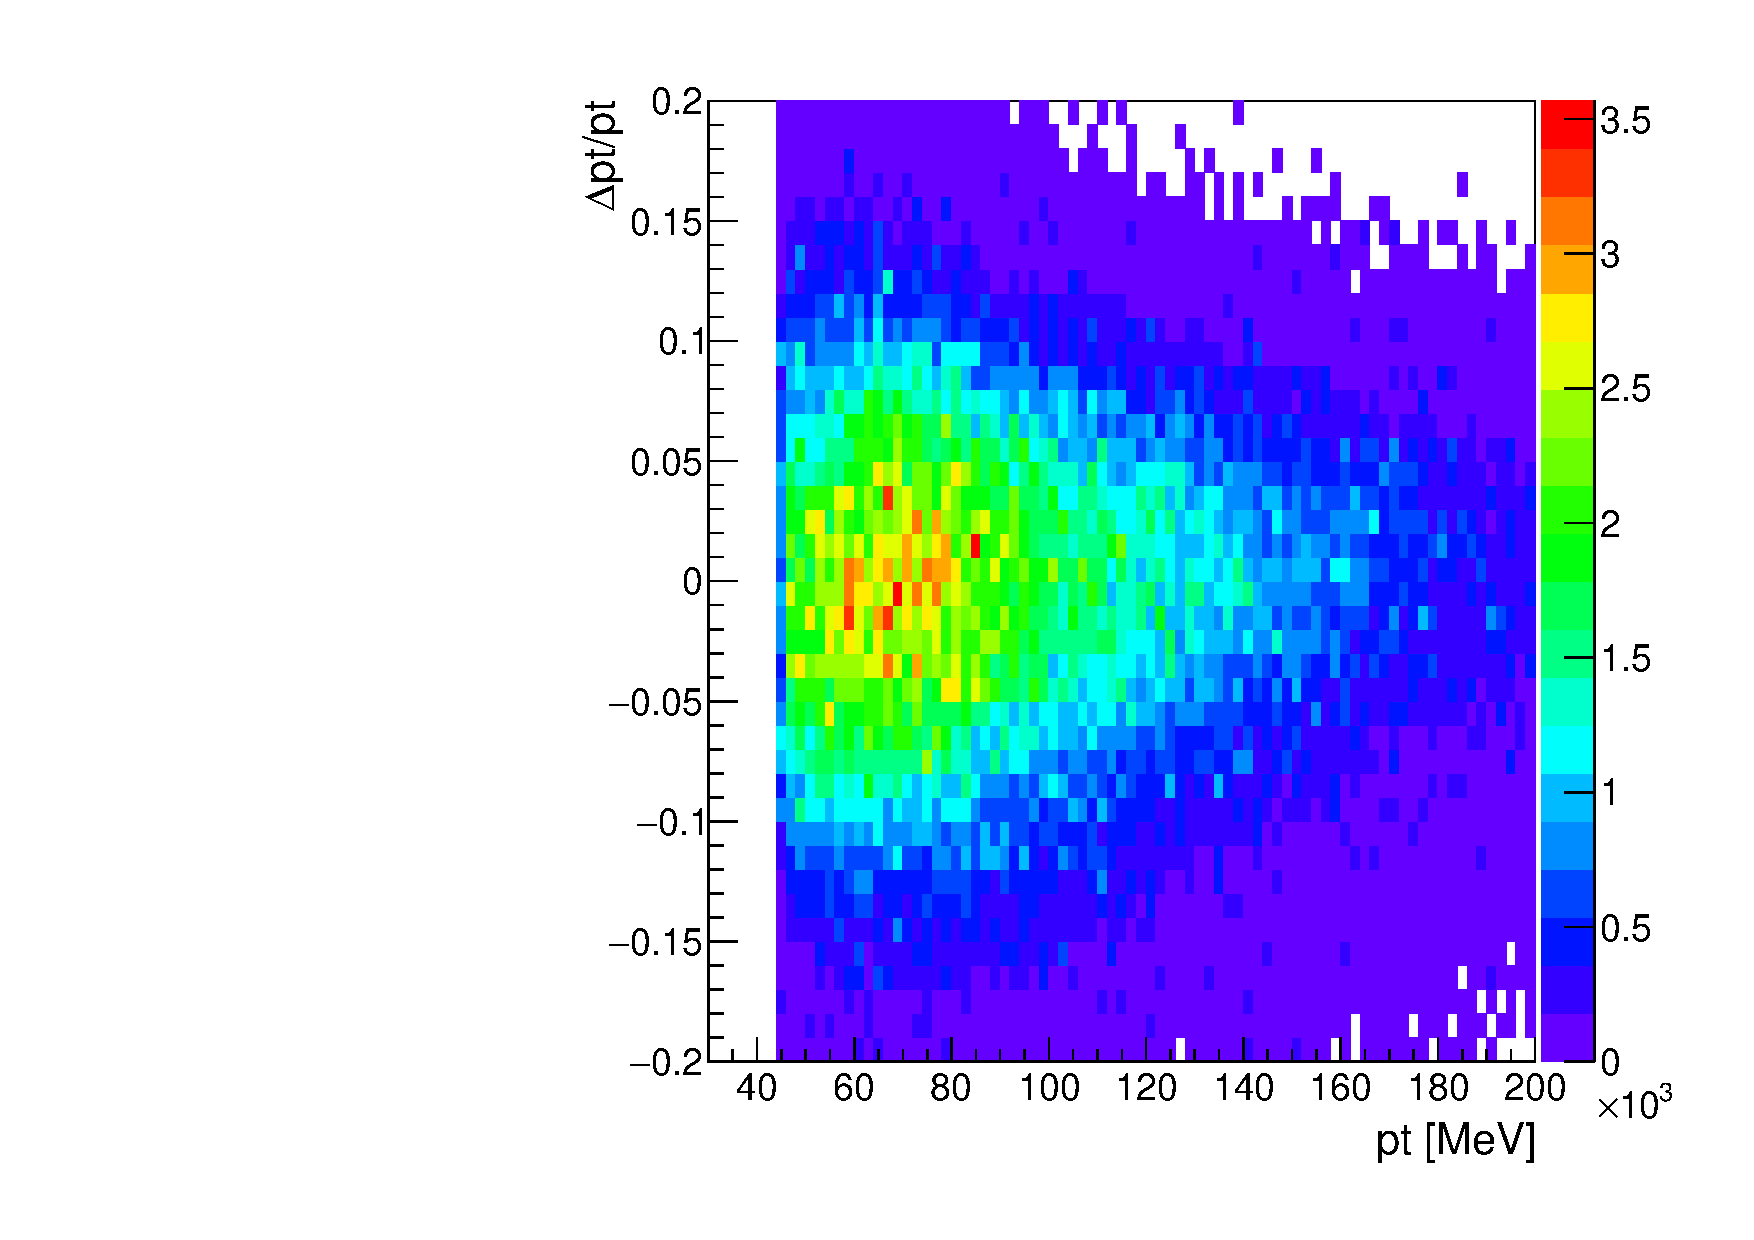
\includegraphics[width=1\linewidth]{ptRatio_Leading_BJet_eta_lower}

			\end{minipage}
			\quad
			\begin{minipage}[h]{0.33\linewidth}
				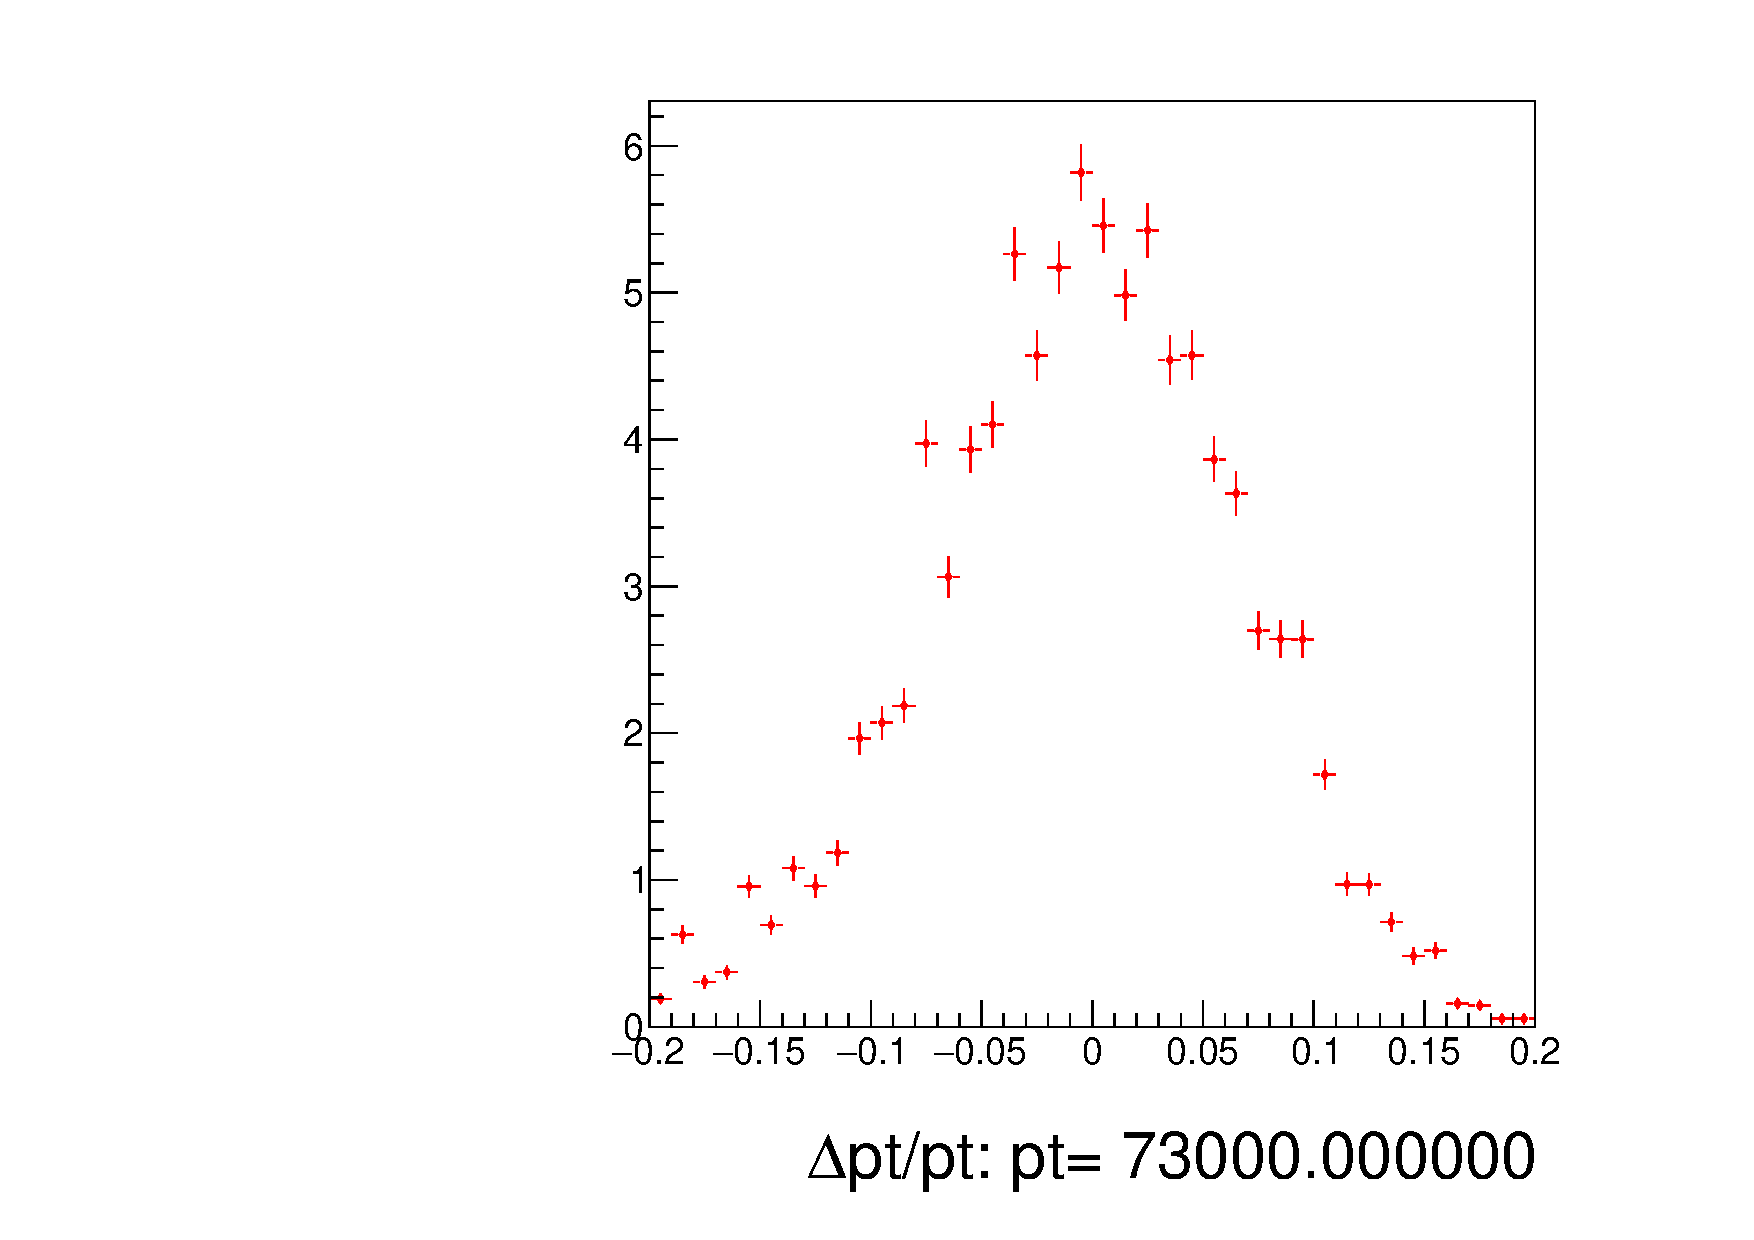
\includegraphics[width=1\linewidth]{ptRatio_Leading_BJet_eta_lower_Slice}
			\end{minipage}
			\caption{$\Delta $\pt$_{ratio}$ for the leading \pt $b$-jet with $0 < \eta < 1$ from MC events against \pt of the offline $b$-jet. A slice across the $y$-axis has been taken at \pt$=79$GeV. }
			\label{fig:MC:leadingbptcentral}
		\end{figure}

		\begin{figure}[h]
			\centering

			\begin{minipage}[h]{0.33\linewidth}
				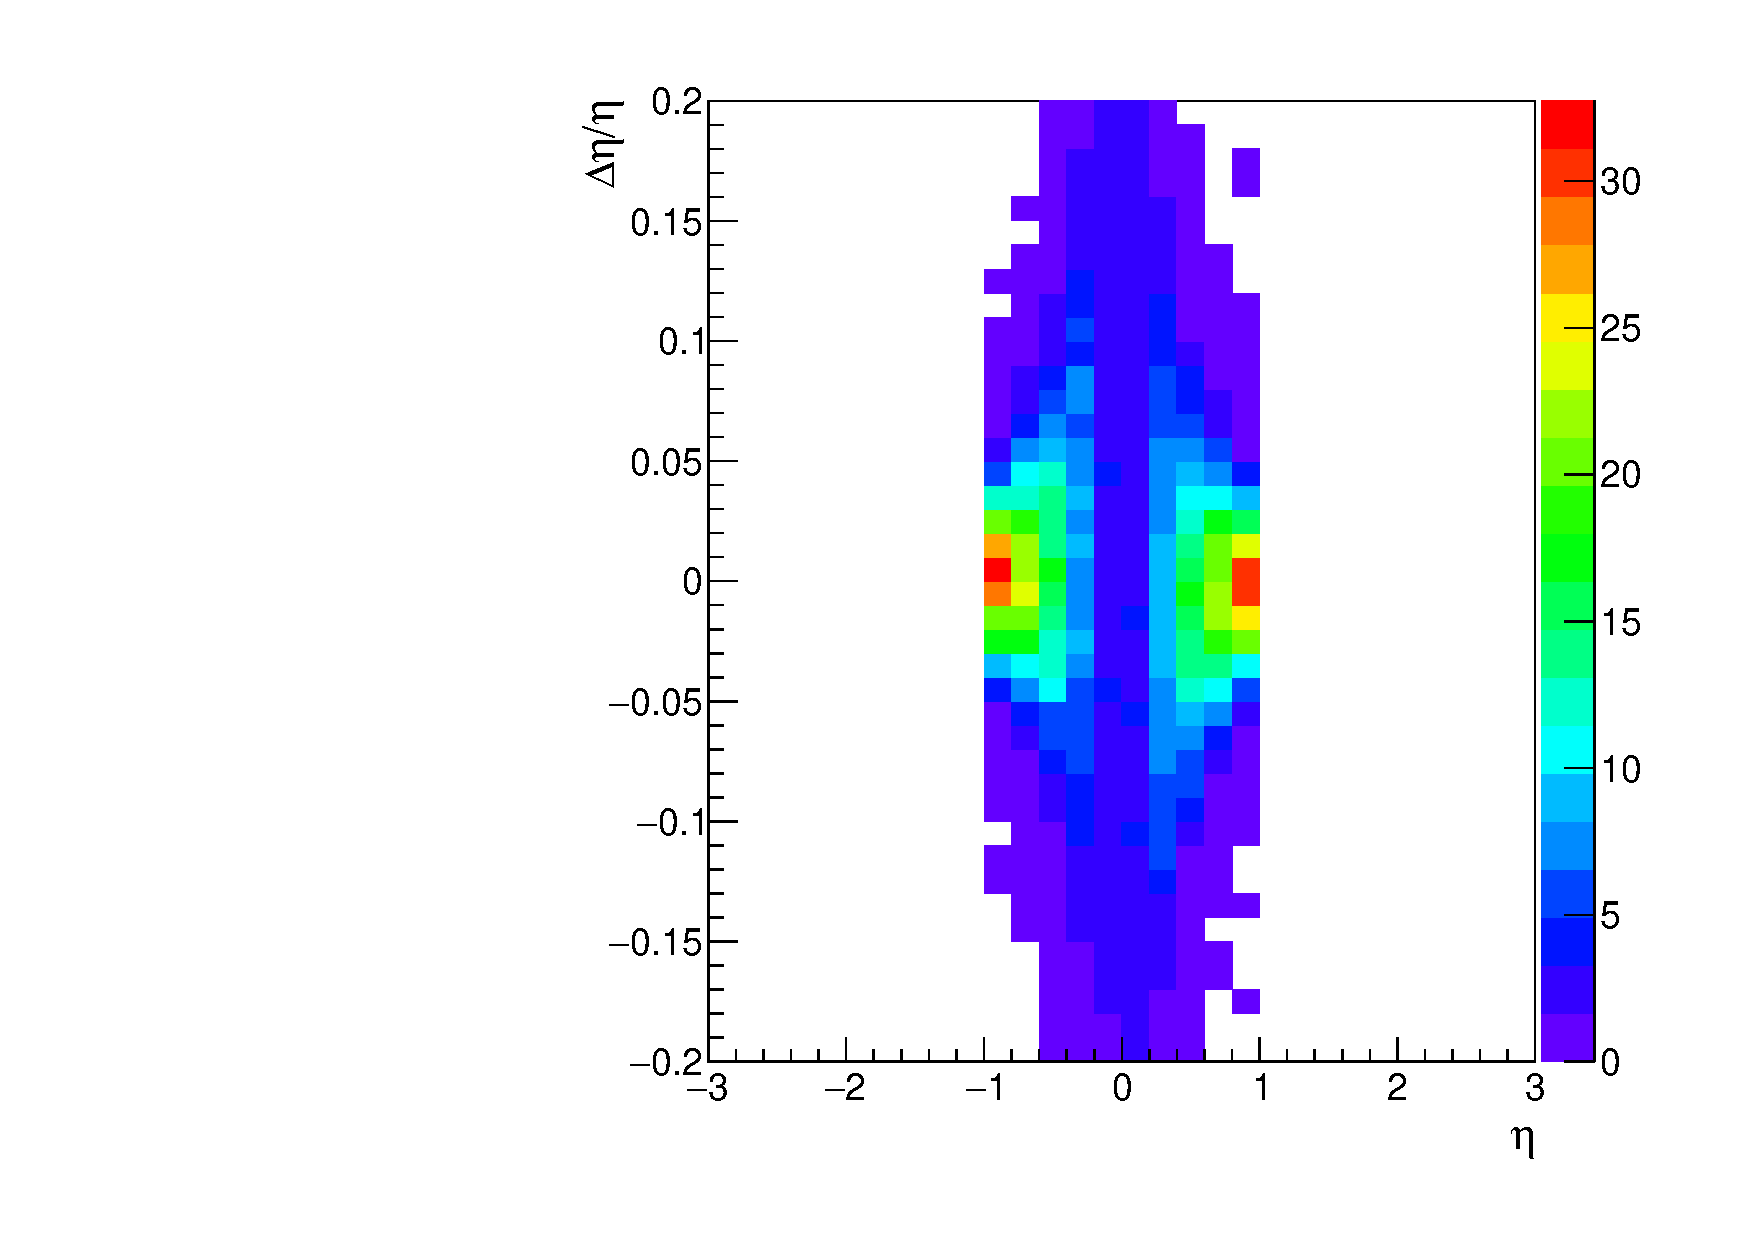
\includegraphics[width=1\linewidth]{etaRatio_Leading_BJet_eta_lower}
			\end{minipage}
			\quad
			\begin{minipage}[h]{0.33\linewidth}
				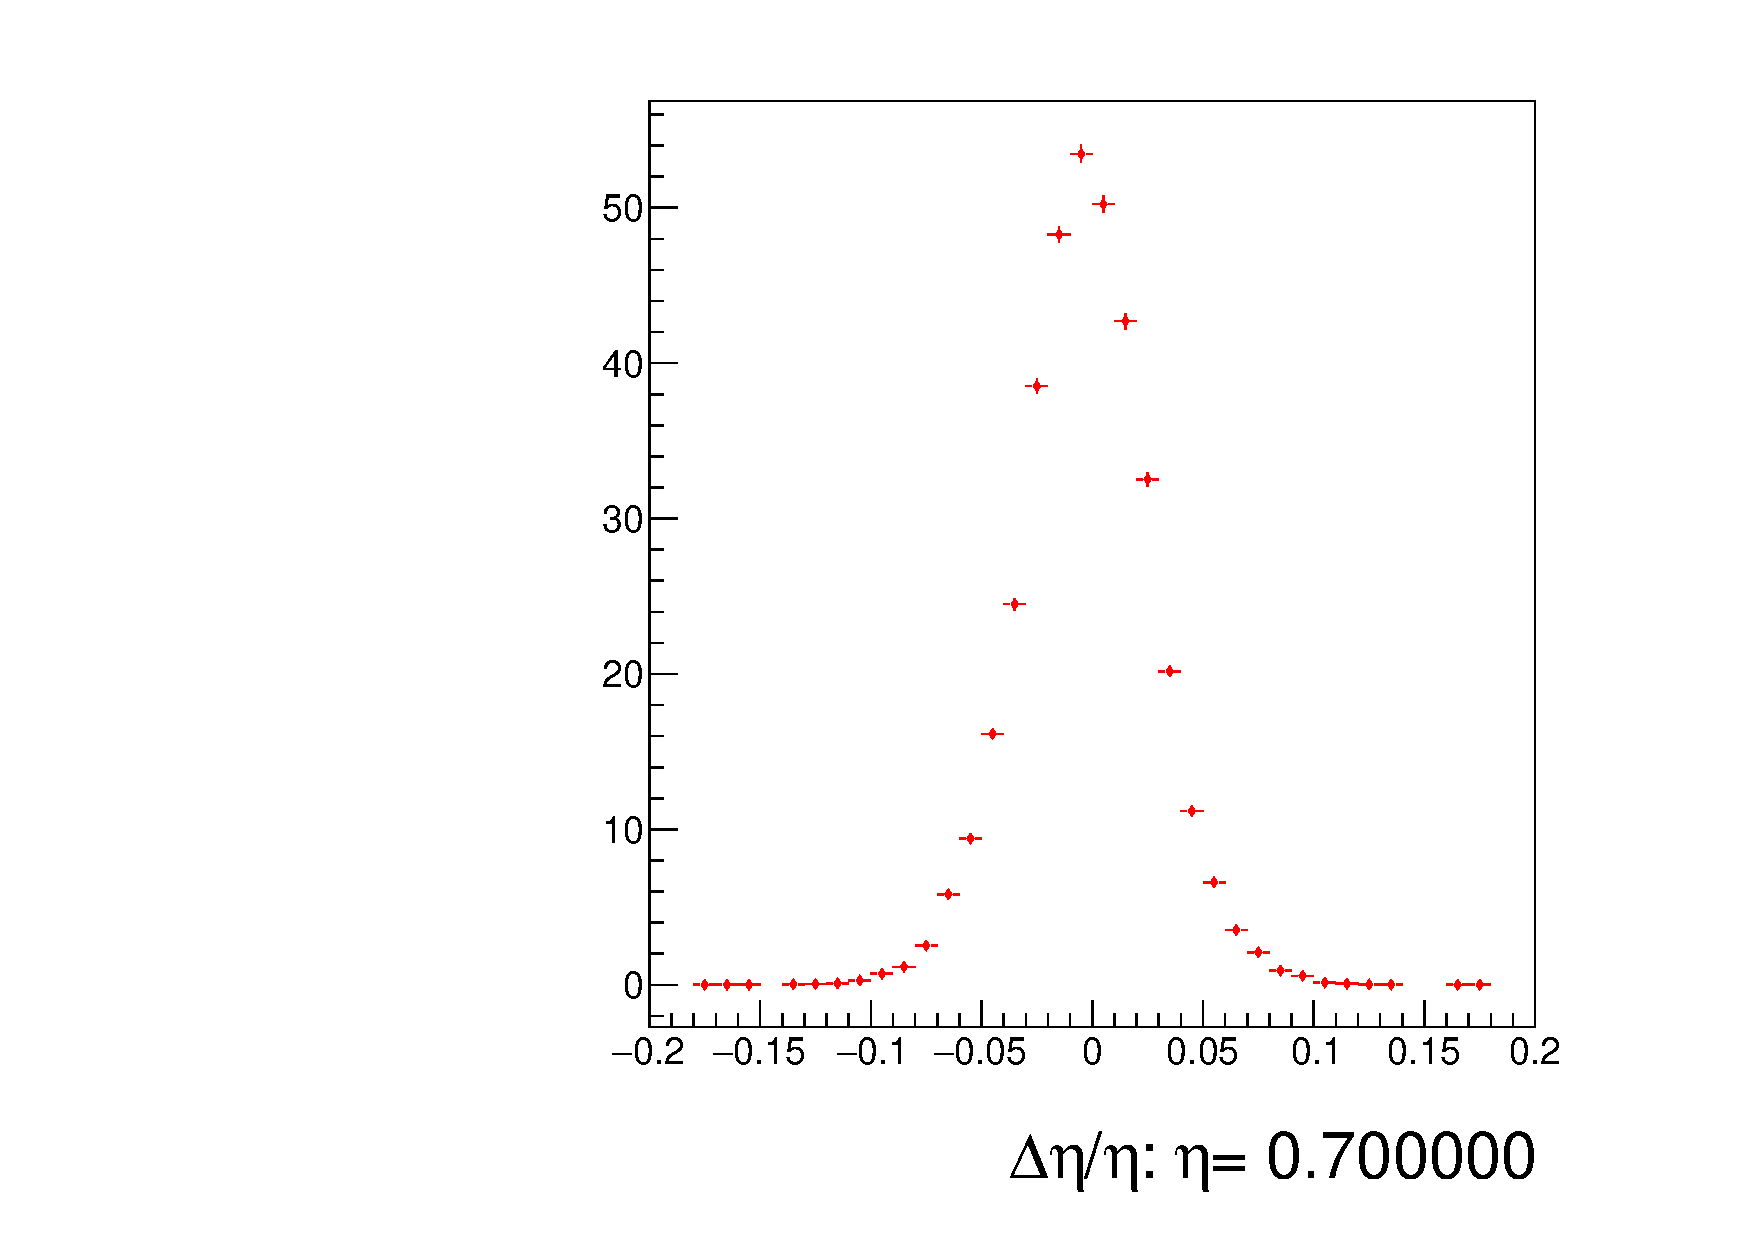
\includegraphics[width=1\linewidth]{etaRatio_Leading_BJet_eta_lower_Slice}
			\end{minipage}
			\caption{$\Delta \eta_{ratio}$ for the leading \pt $b$-jet with $0 < \eta < 1$ from MC events against $\eta$ of the offline $b$-jet. A slice across the $y$-axis has been taken at $\eta=-1.9$. }
			\label{fig:MC:leadingbetacentral}
		\end{figure}

		\begin{figure}[h]
			\centering

			\begin{minipage}[h]{0.33\linewidth}
				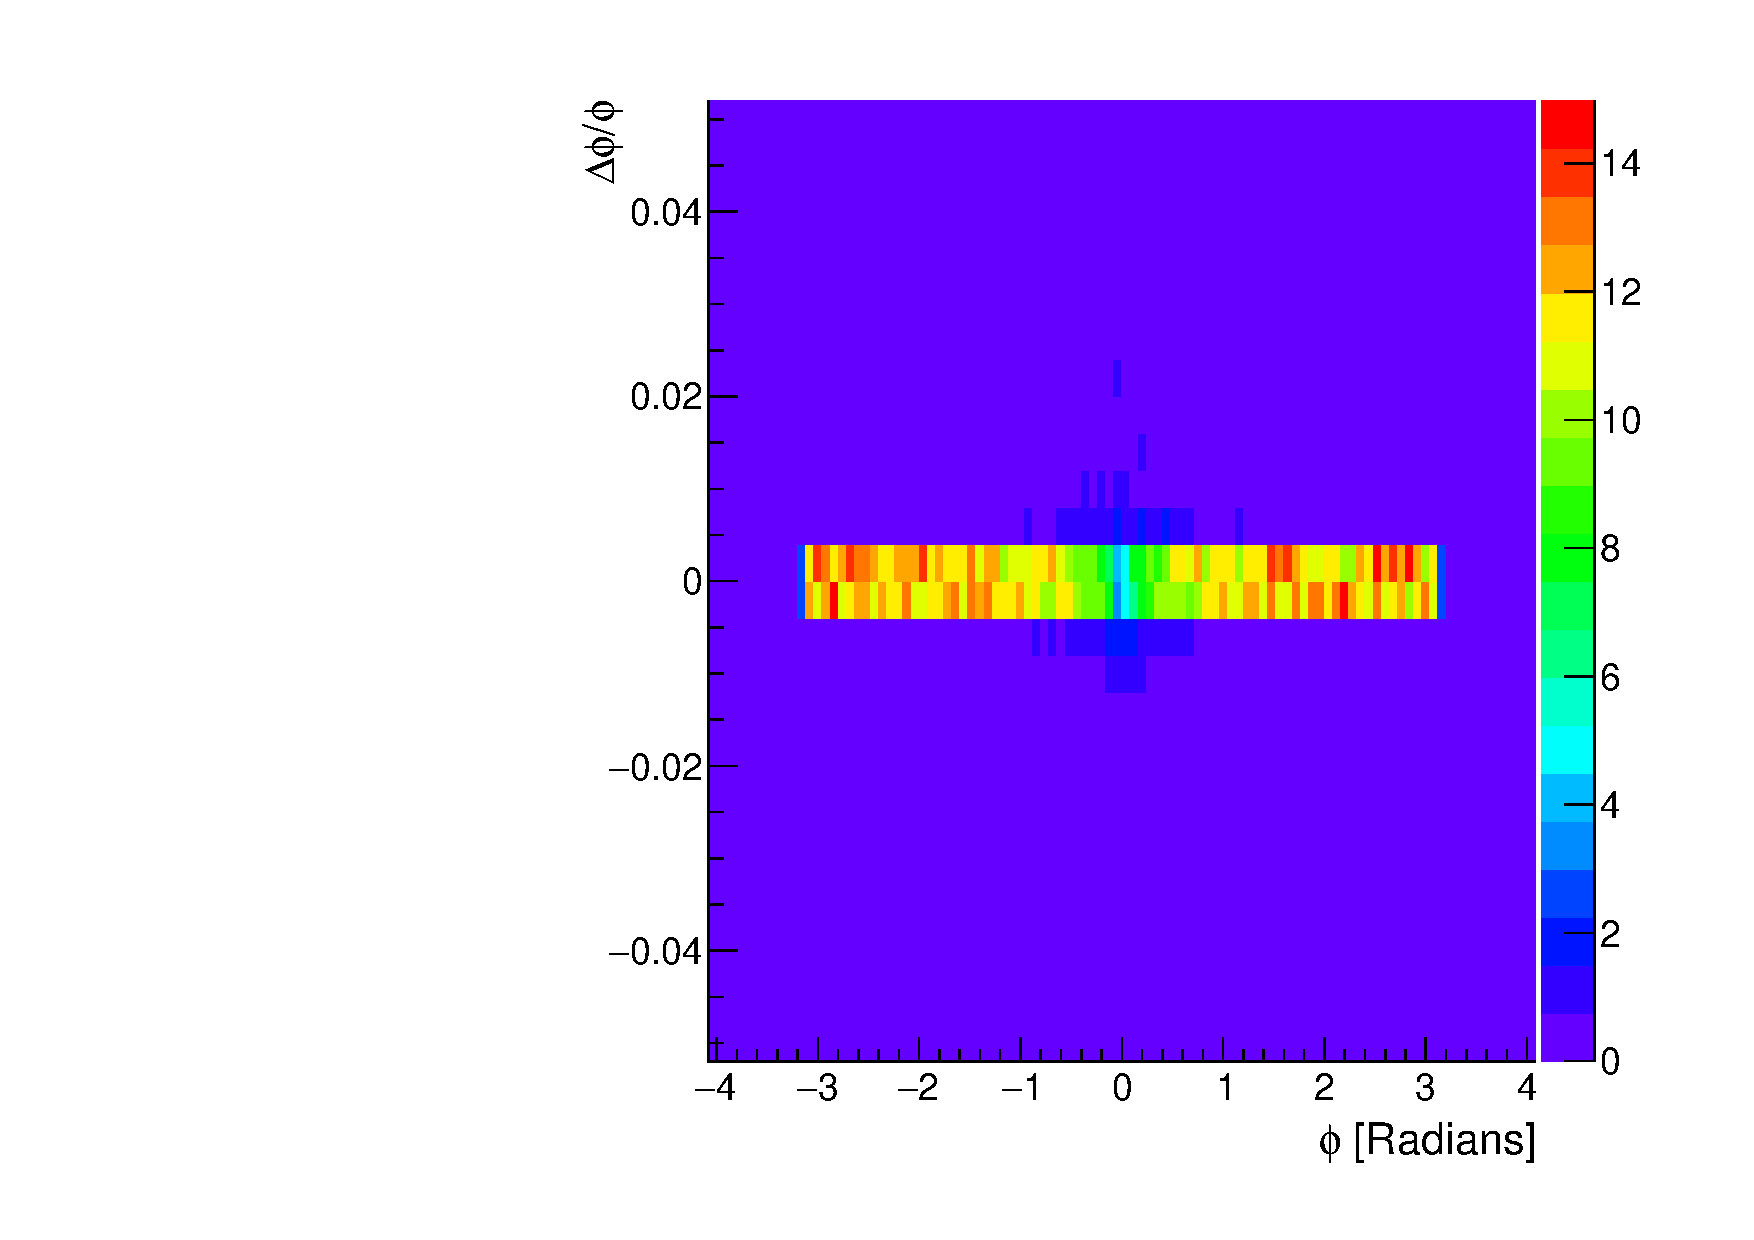
\includegraphics[width=1\linewidth]{phiRatio_Leading_BJet_eta_lower}
			\end{minipage}
			\quad
			\begin{minipage}[h]{0.33\linewidth}
				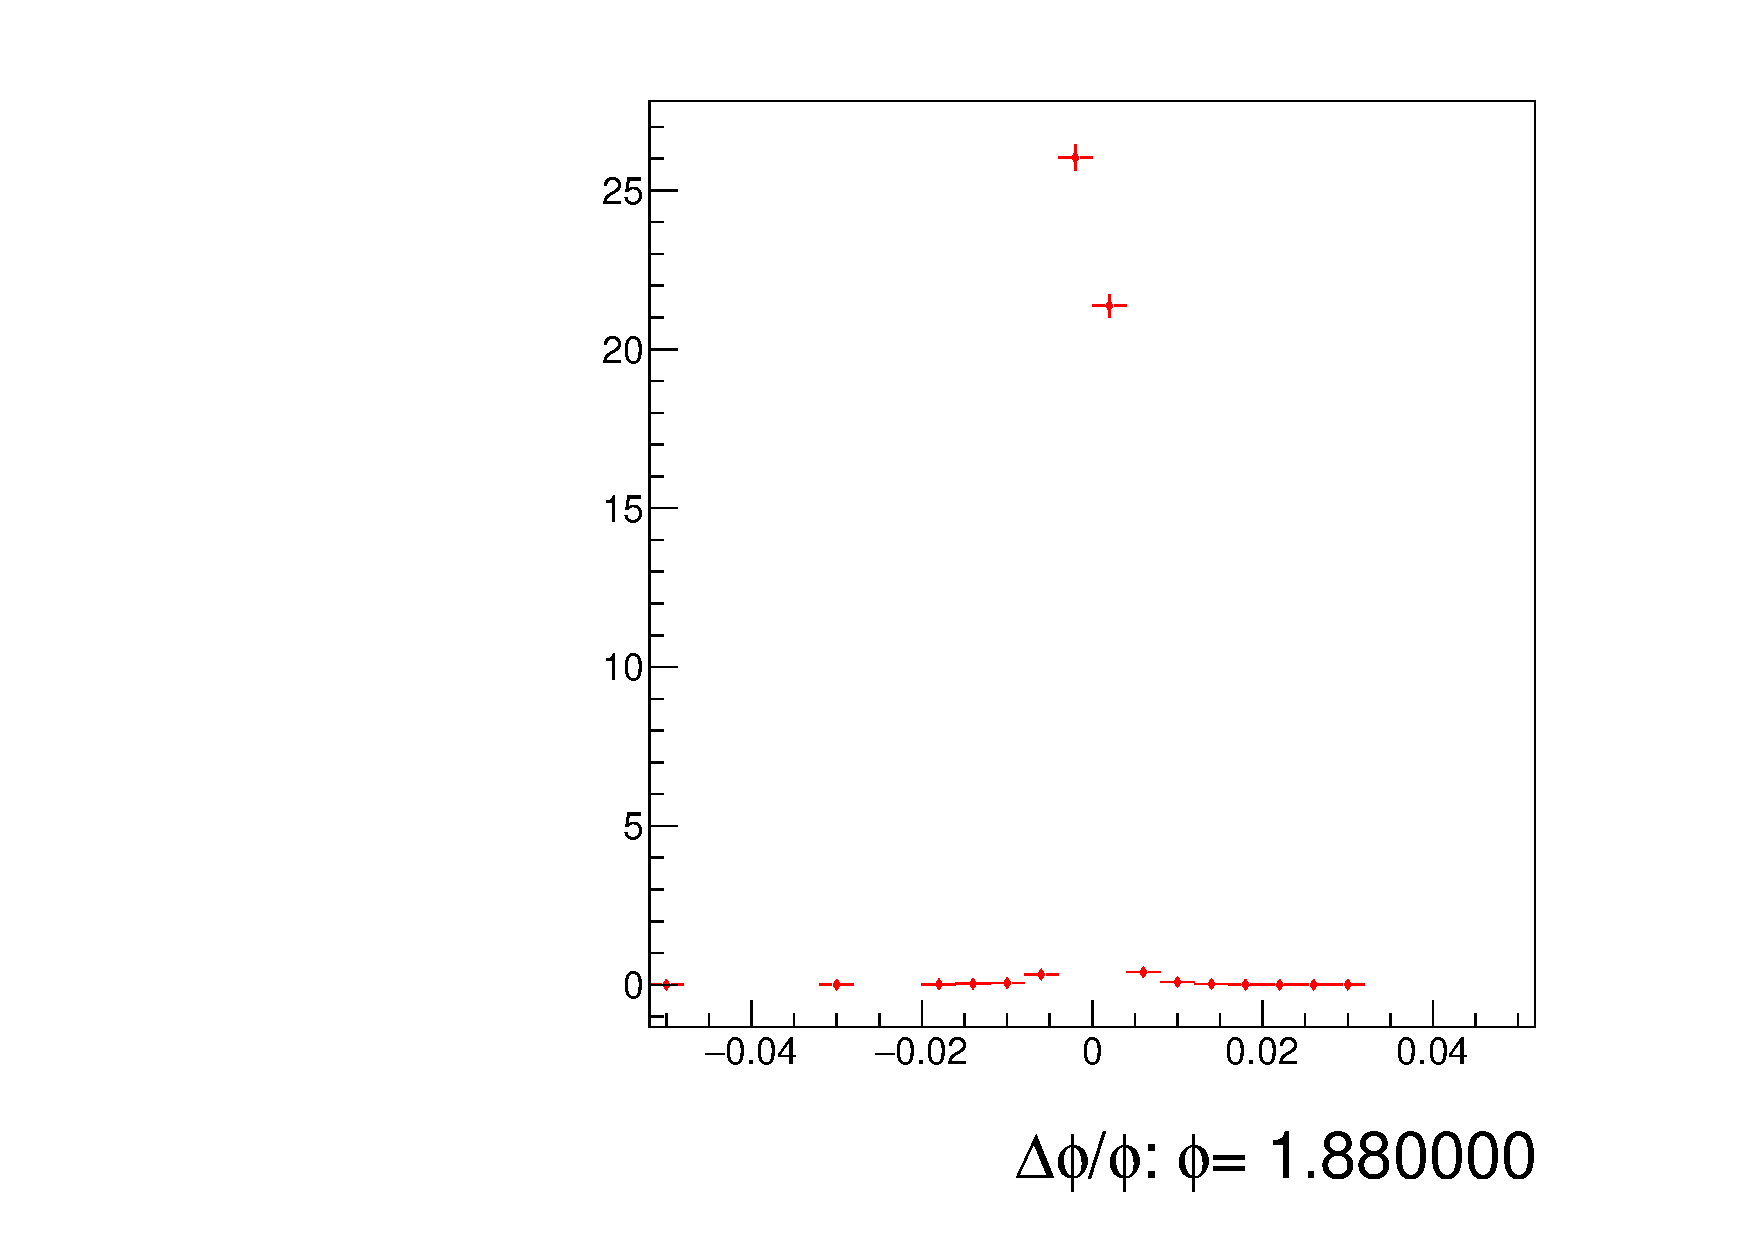
\includegraphics[width=1\linewidth]{phiRatio_Leading_BJet_eta_lower_Slice}
			\end{minipage}
			\caption{$\Delta \phi_{ratio}$ for the leading \pt $b$-jet with $0 < \eta < 1$ from MC events against $\phi$ of the offline $b$-jet. A slice across the $y$-axis has been taken at $\phi=-1.64$. }
			\label{fig:MC:leadingbphicentral}
		\end{figure}

		\begin{figure}[h]
			\centering

			\begin{minipage}[h]{0.33\linewidth}
				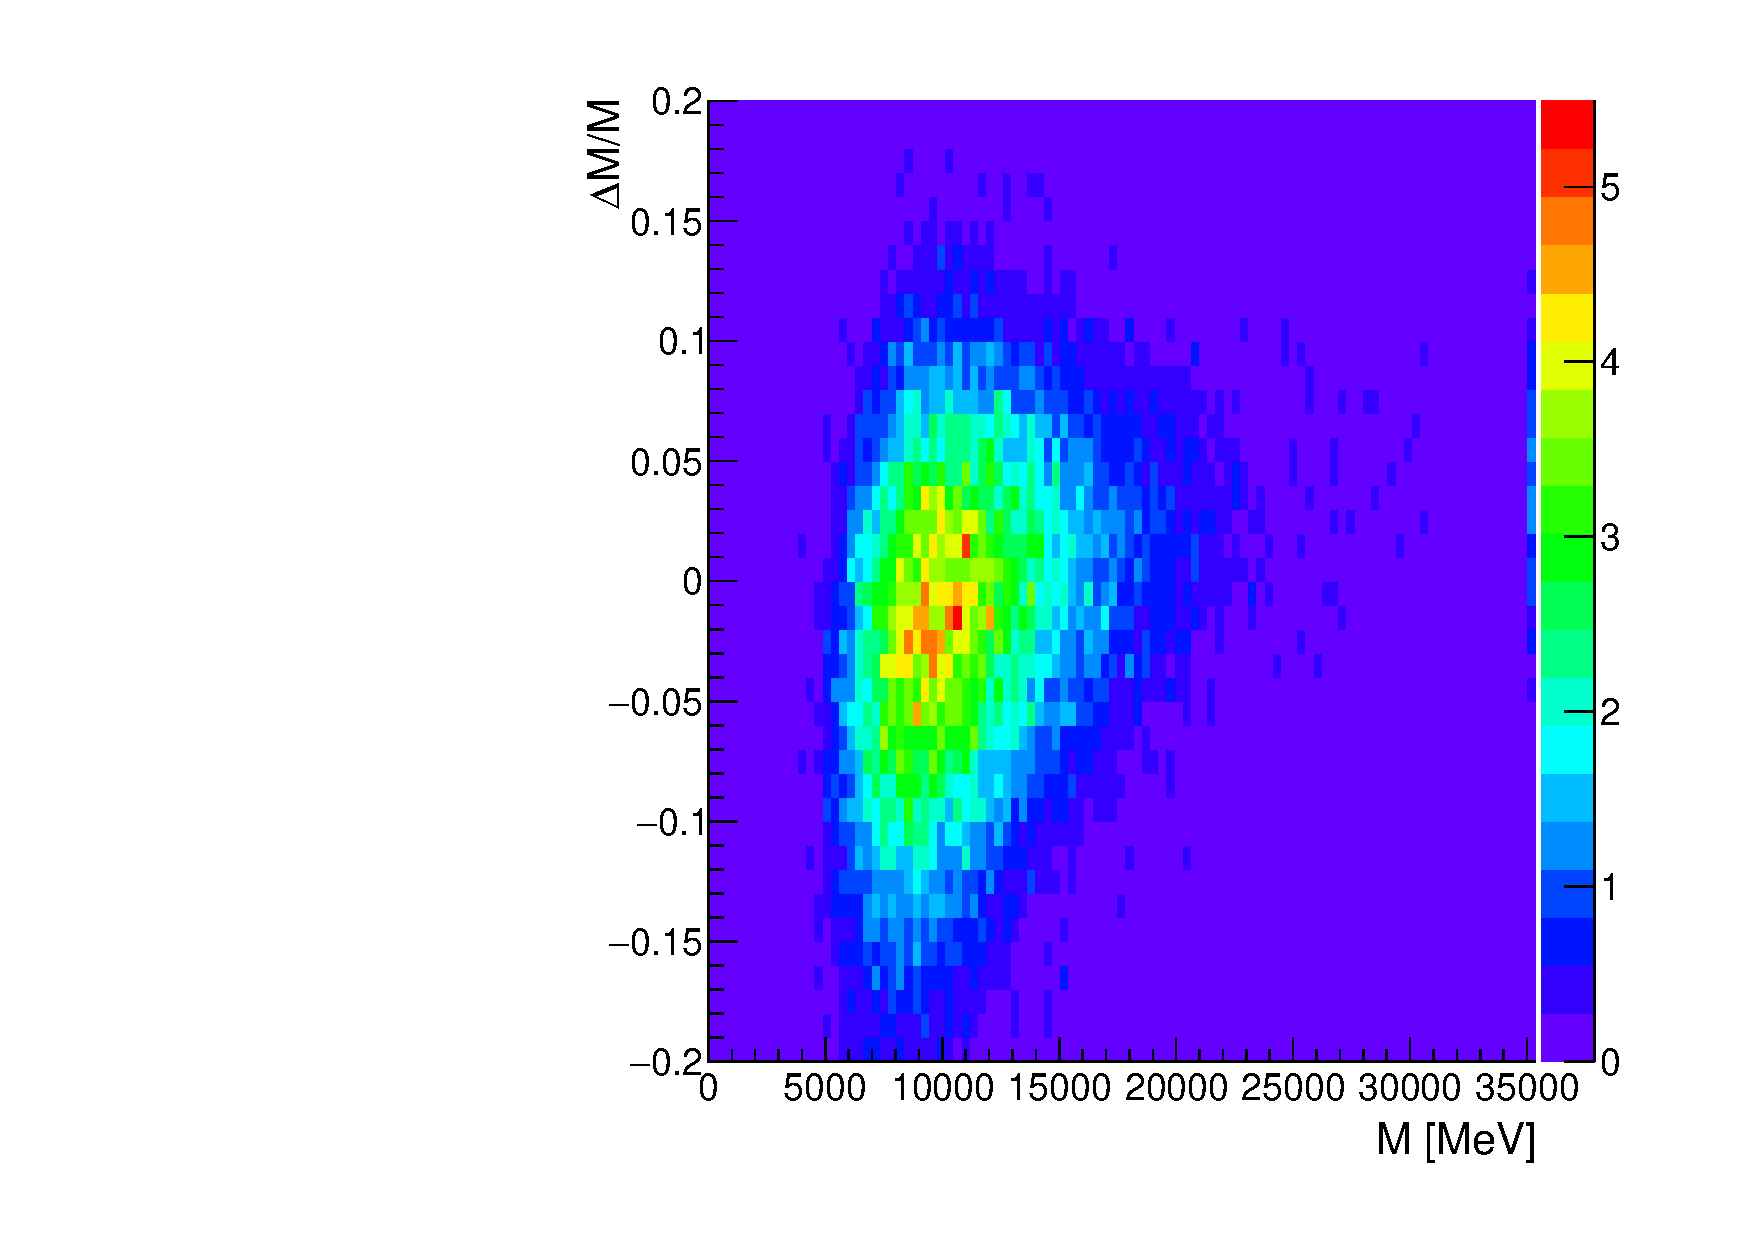
\includegraphics[width=1\linewidth]{mRatio_Leading_BJet_eta_lower}
			\end{minipage}
			\quad
			\begin{minipage}[h]{0.33\linewidth}
				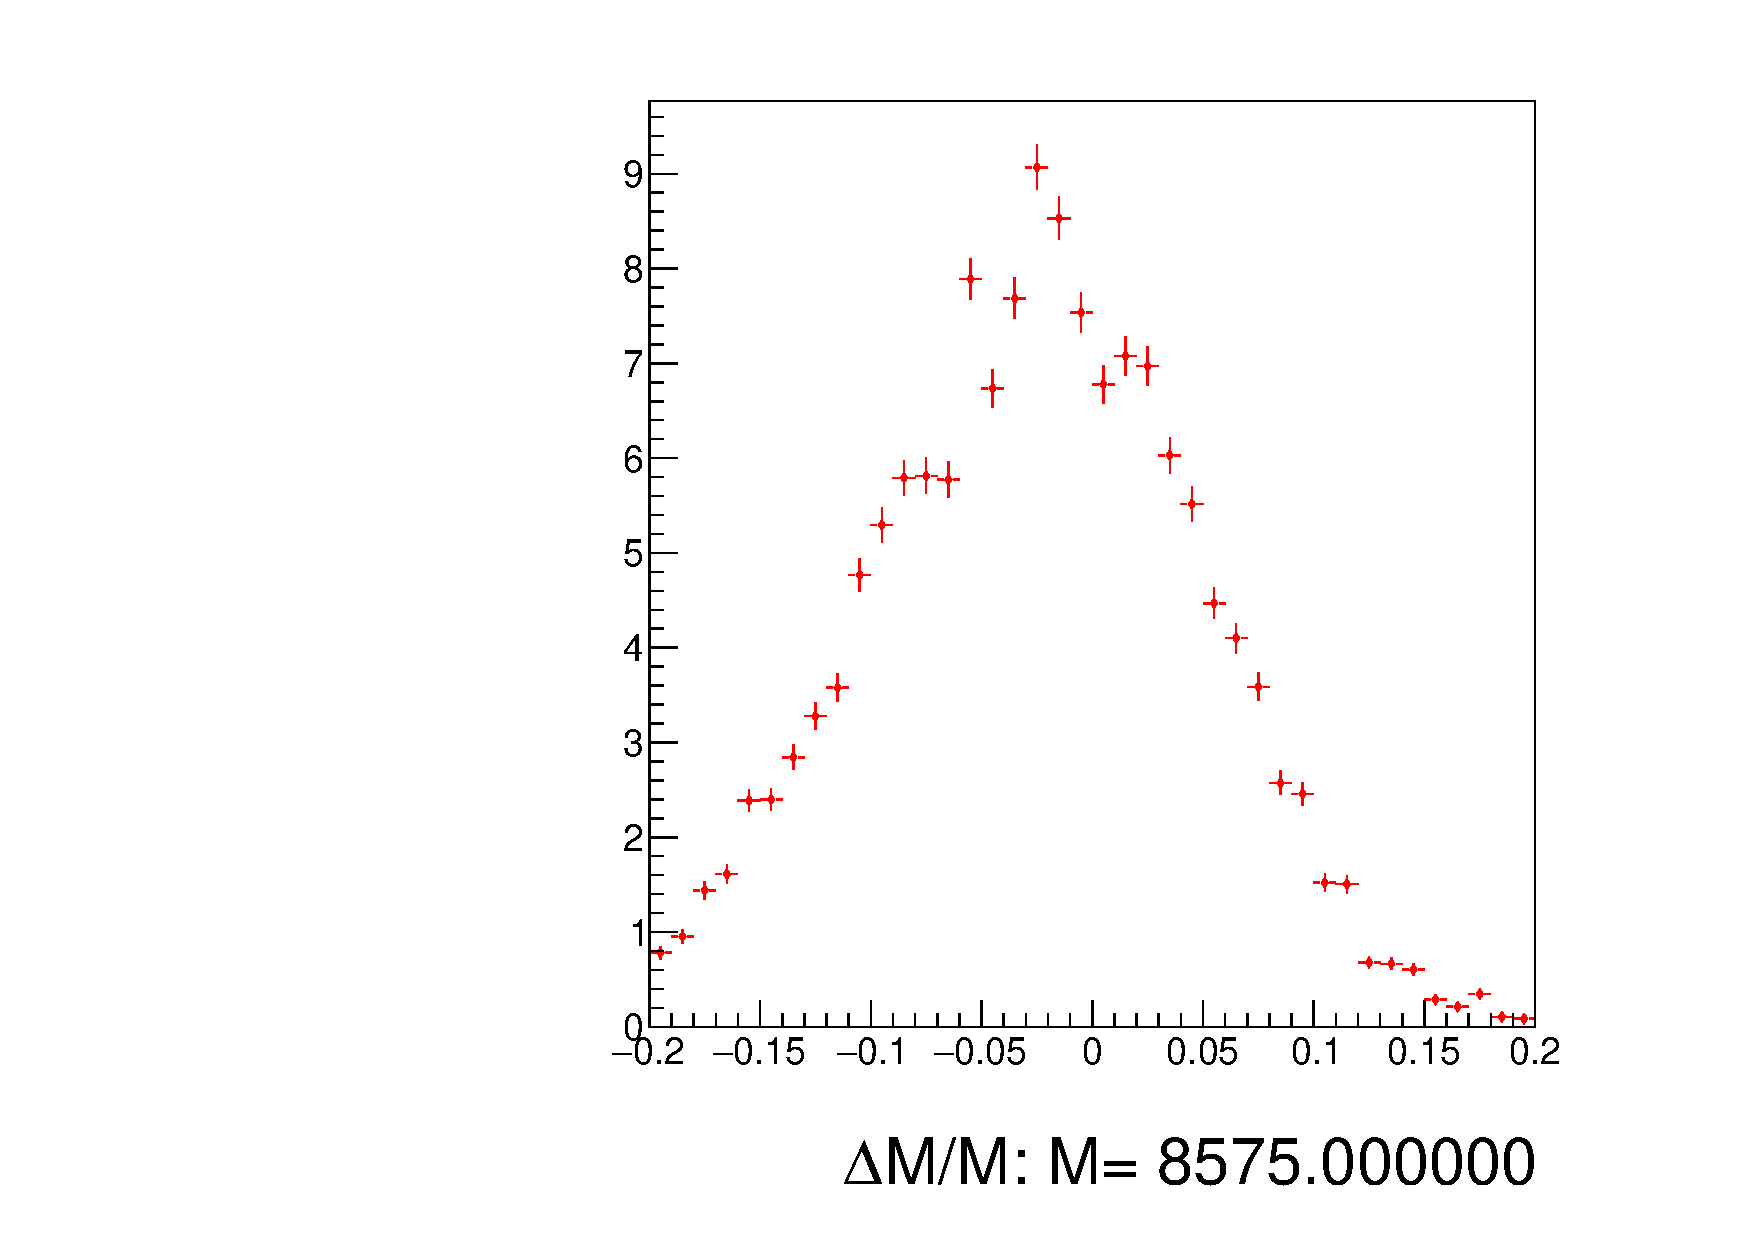
\includegraphics[width=1\linewidth]{mRatio_Leading_BJet_eta_lower_Slice}
			\end{minipage}
			\caption{$\Delta M_{ratio}$ for the leading \pt $b$-jet with $0 < \eta < 1$ from MC events against $M$ of the offline $b$-jet. A slice across the $y$-axis has been taken at $M=7$GeV. }
			\label{fig:MC:leadingbmcentral}
		\end{figure}

\newpage
		\subsection{Data}
		
				\begin{figure}[h]
					\centering
					\begin{minipage}[h]{0.33\linewidth}
						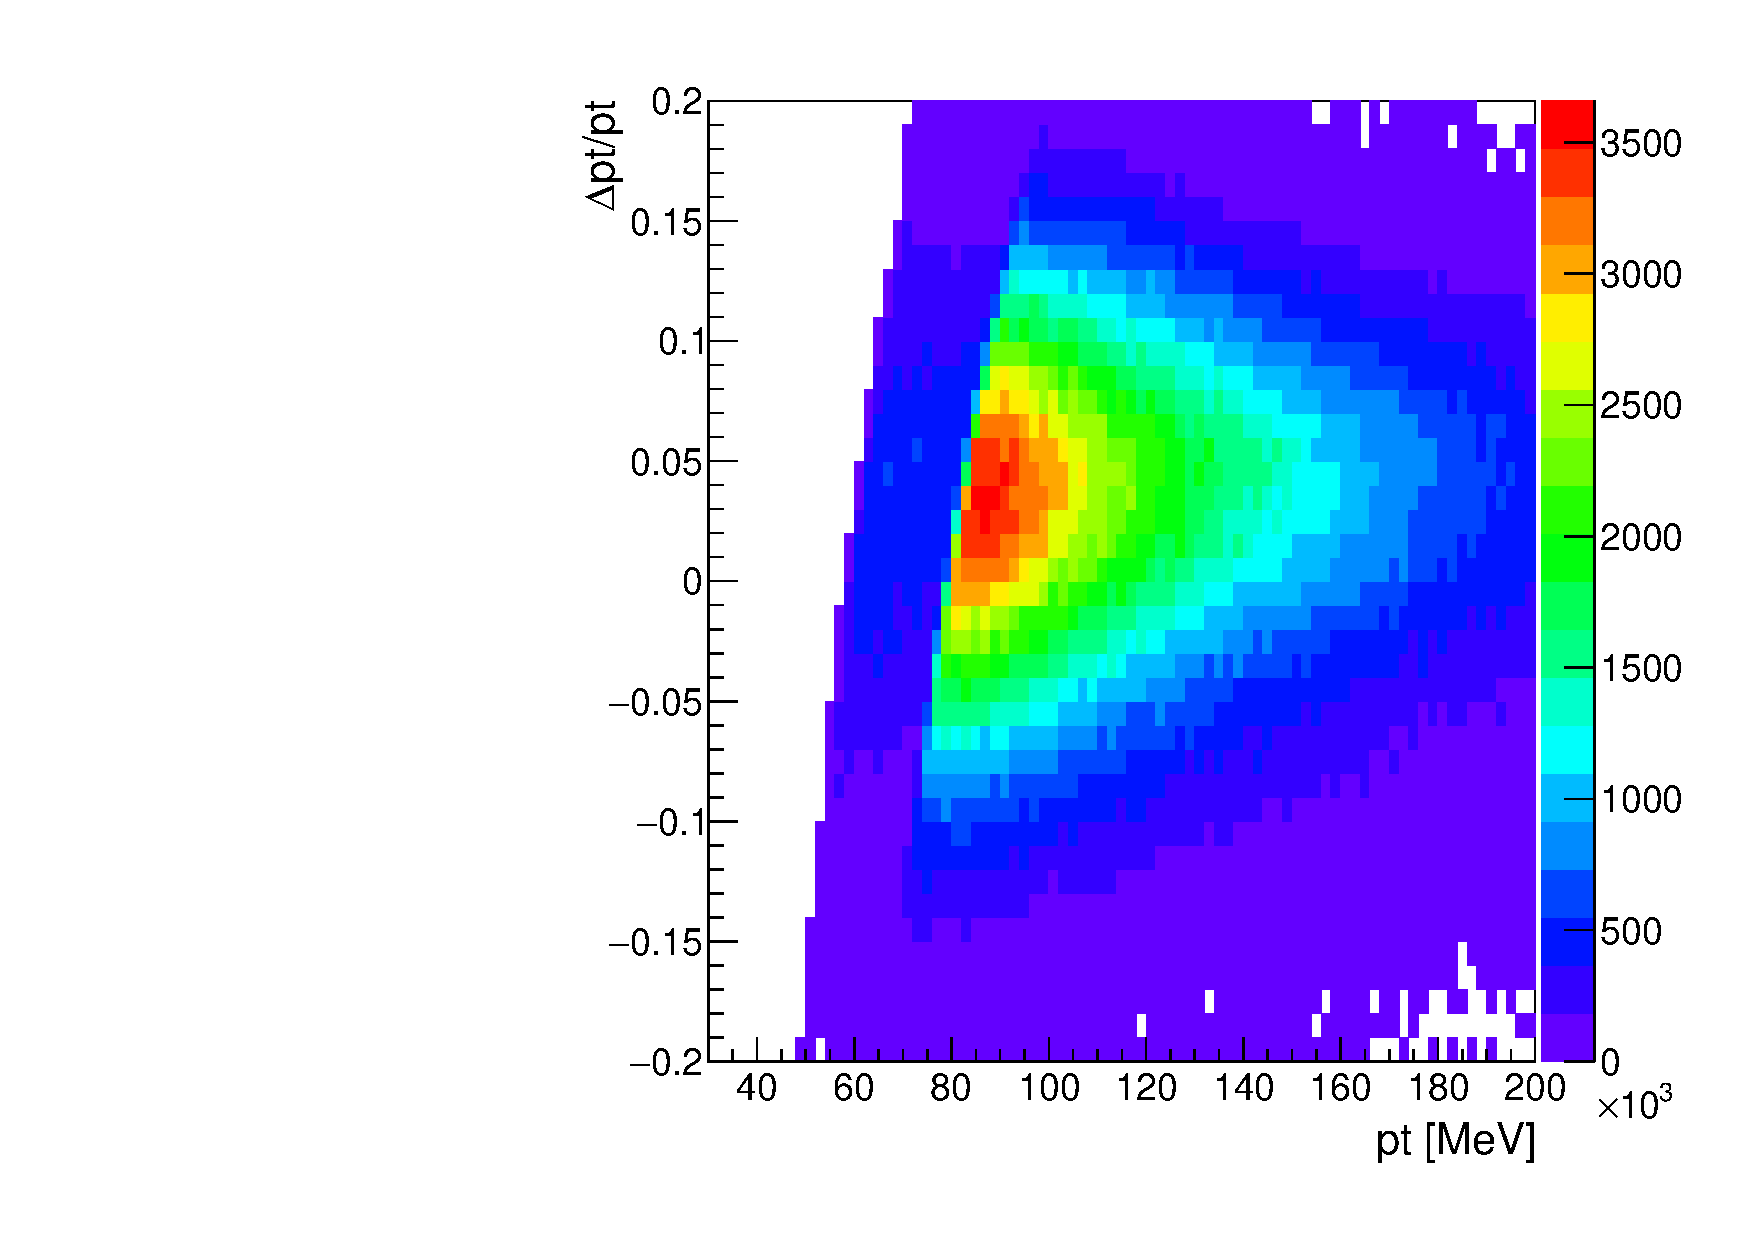
\includegraphics[width=1\linewidth]{Offline_2C_ptRatio_Leading_BJet_eta_lower}
						
					\end{minipage}
					\quad
					\begin{minipage}[h]{0.33\linewidth}
						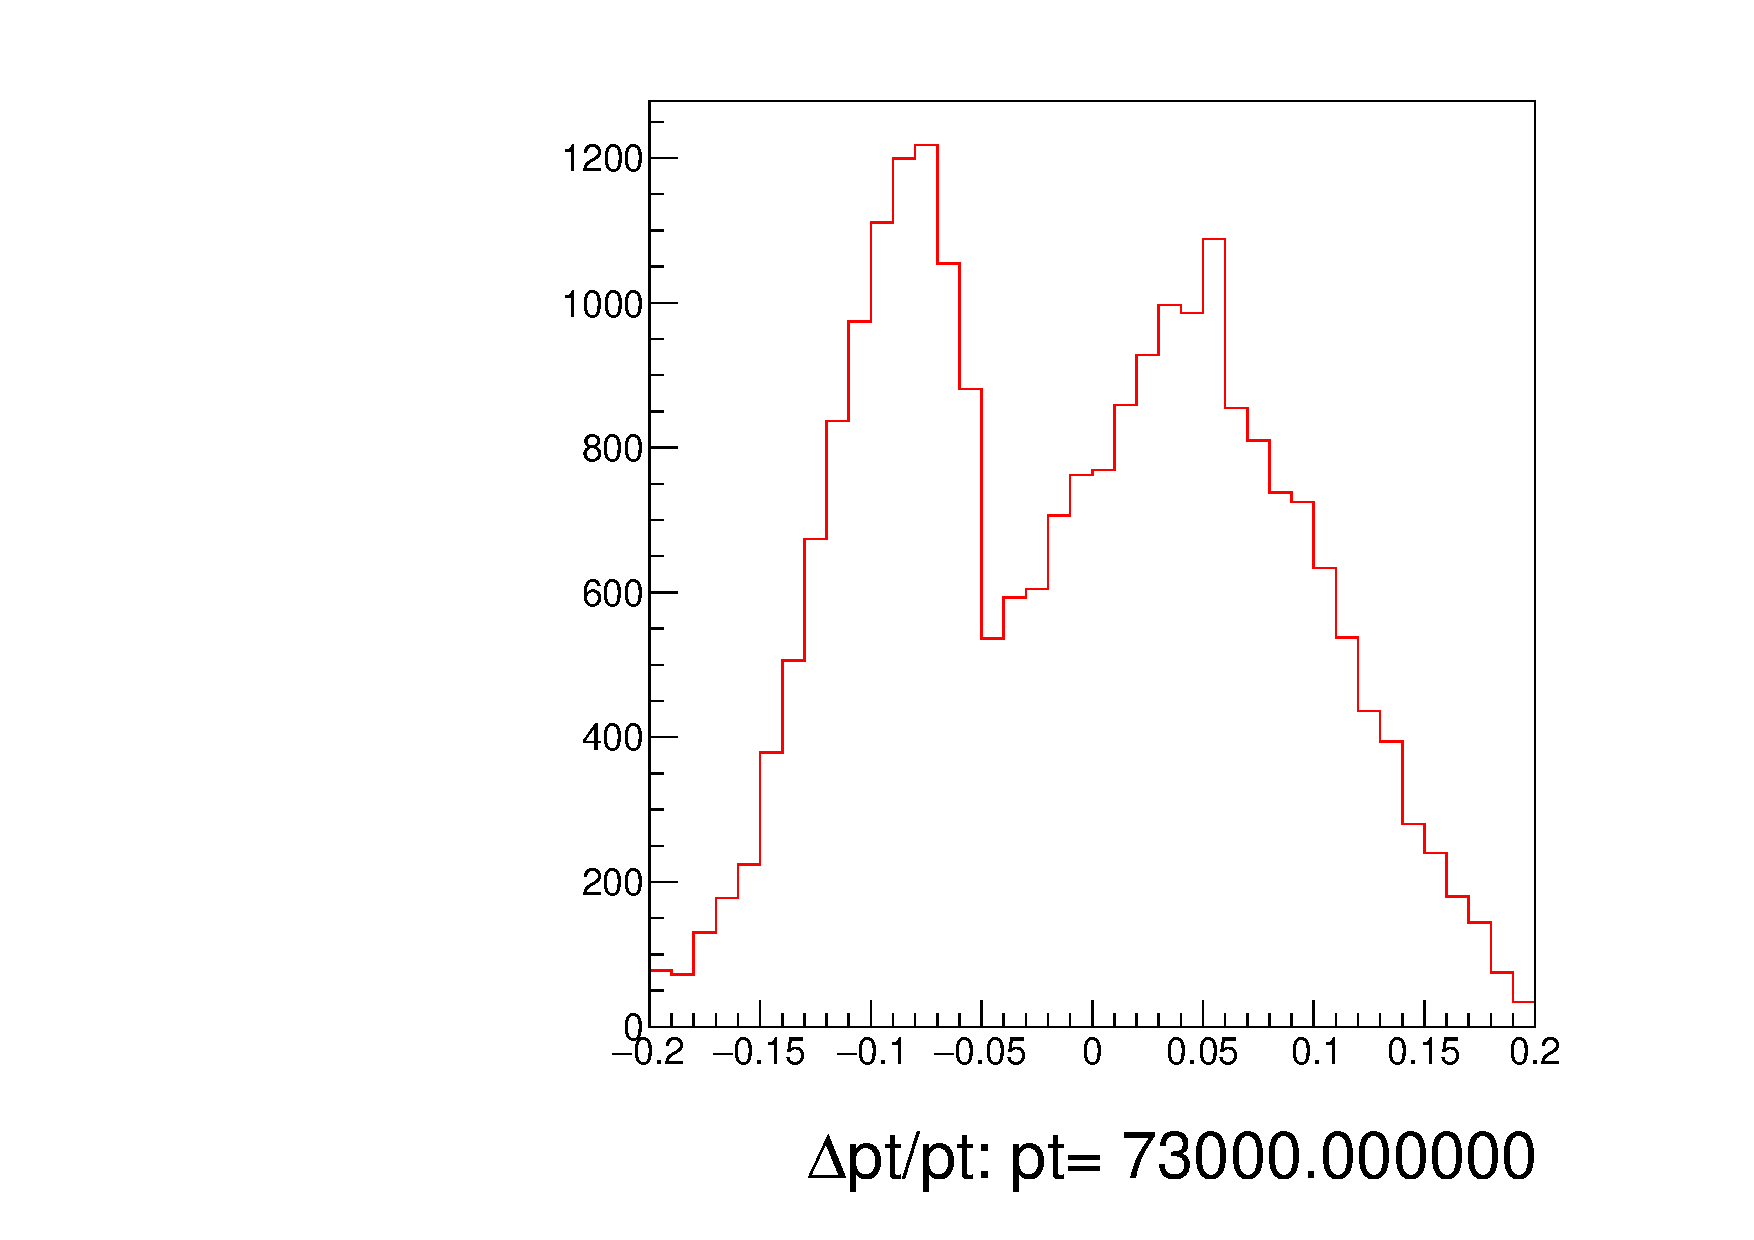
\includegraphics[width=1\linewidth]{Offline_2C_ptRatio_Leading_BJet_eta_lower_Slice}
					\end{minipage}
					\caption{$\Delta $\pt$_{ratio}$ for the leading \pt $b$-jet with $0 < \eta < 1$ from Data events against \pt of the offline $b$-jet. A slice across the $y$-axis has been taken at \pt$=79$GeV. }
					\label{fig:D:leadingbptcentral}
				\end{figure}
				
				\begin{figure}[h]
					\centering
					
					\begin{minipage}[h]{0.33\linewidth}
						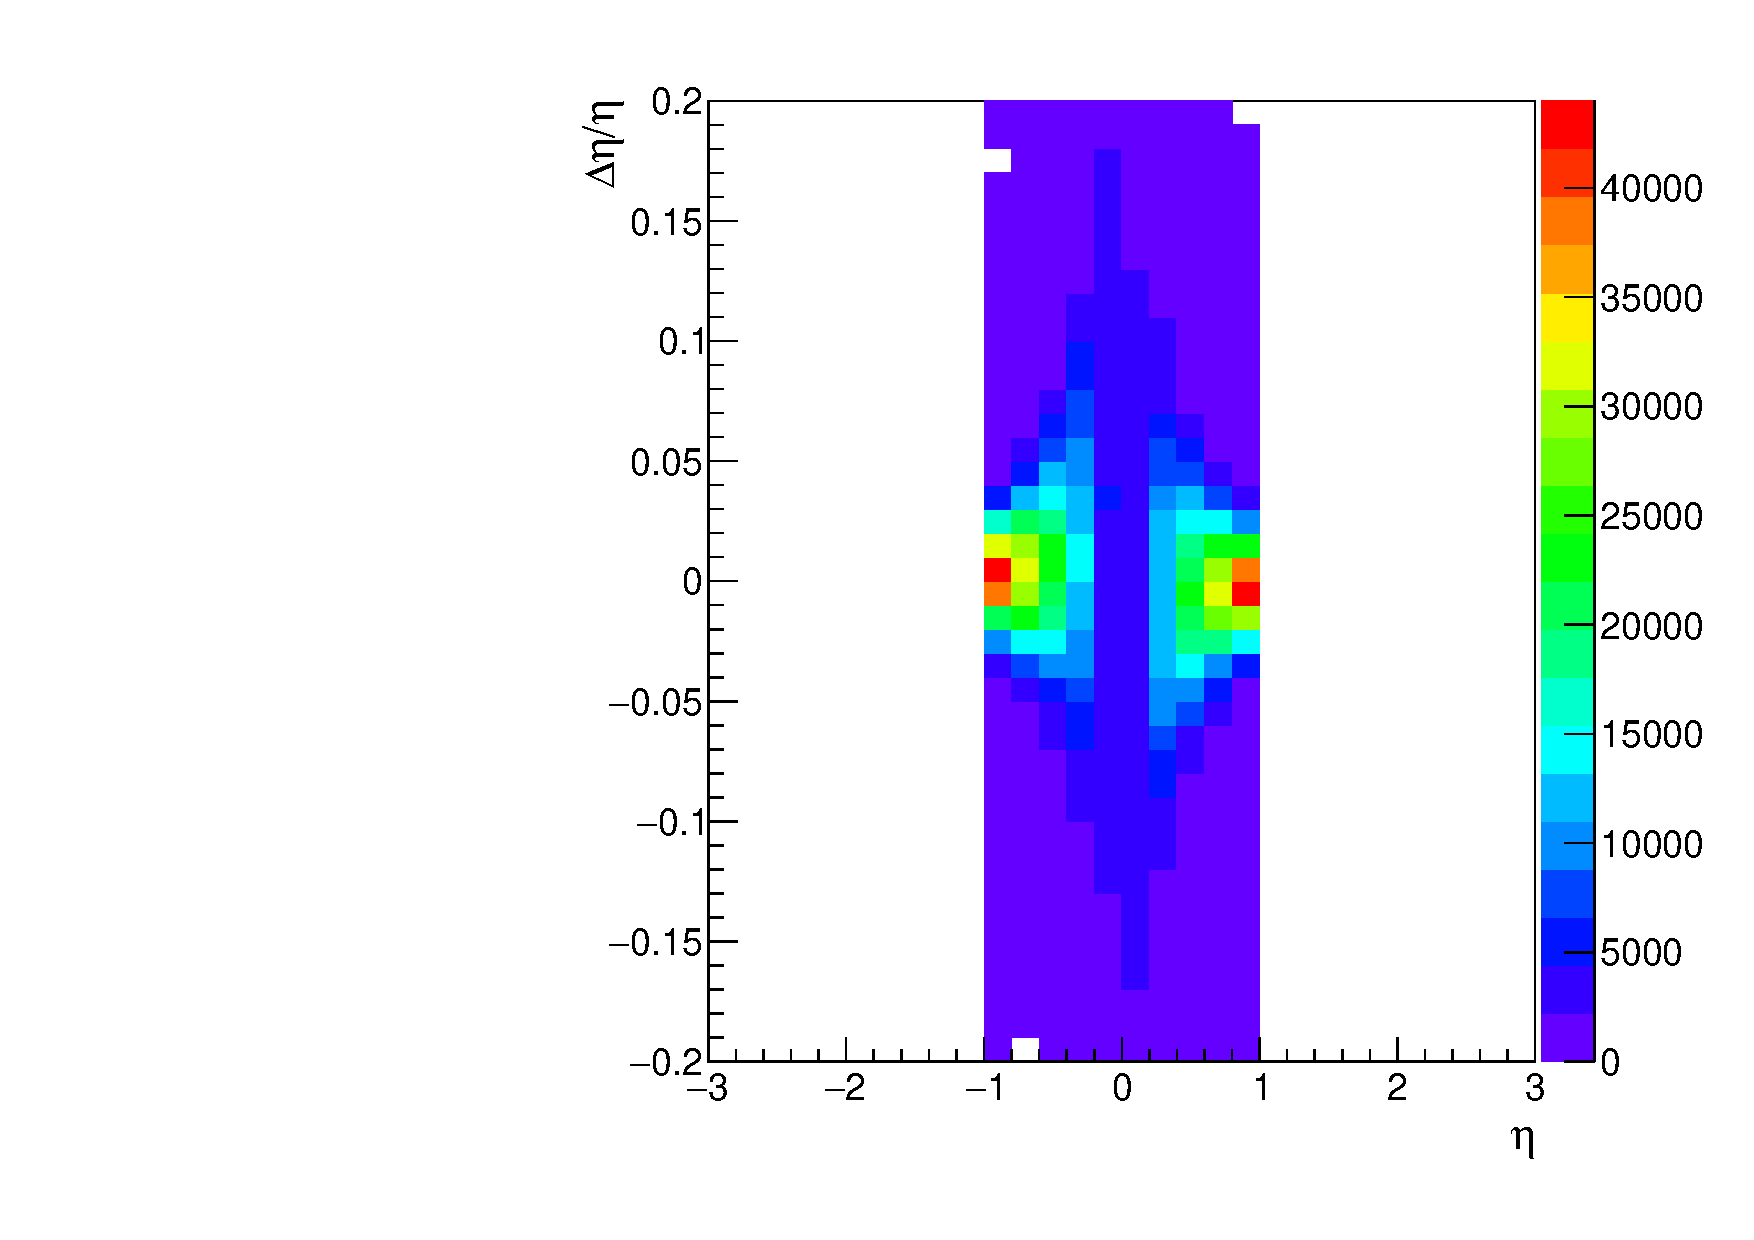
\includegraphics[width=1\linewidth]{Offline_2C_etaRatio_Leading_BJet_eta_lower}
					\end{minipage}
					\quad
					\begin{minipage}[h]{0.33\linewidth}
						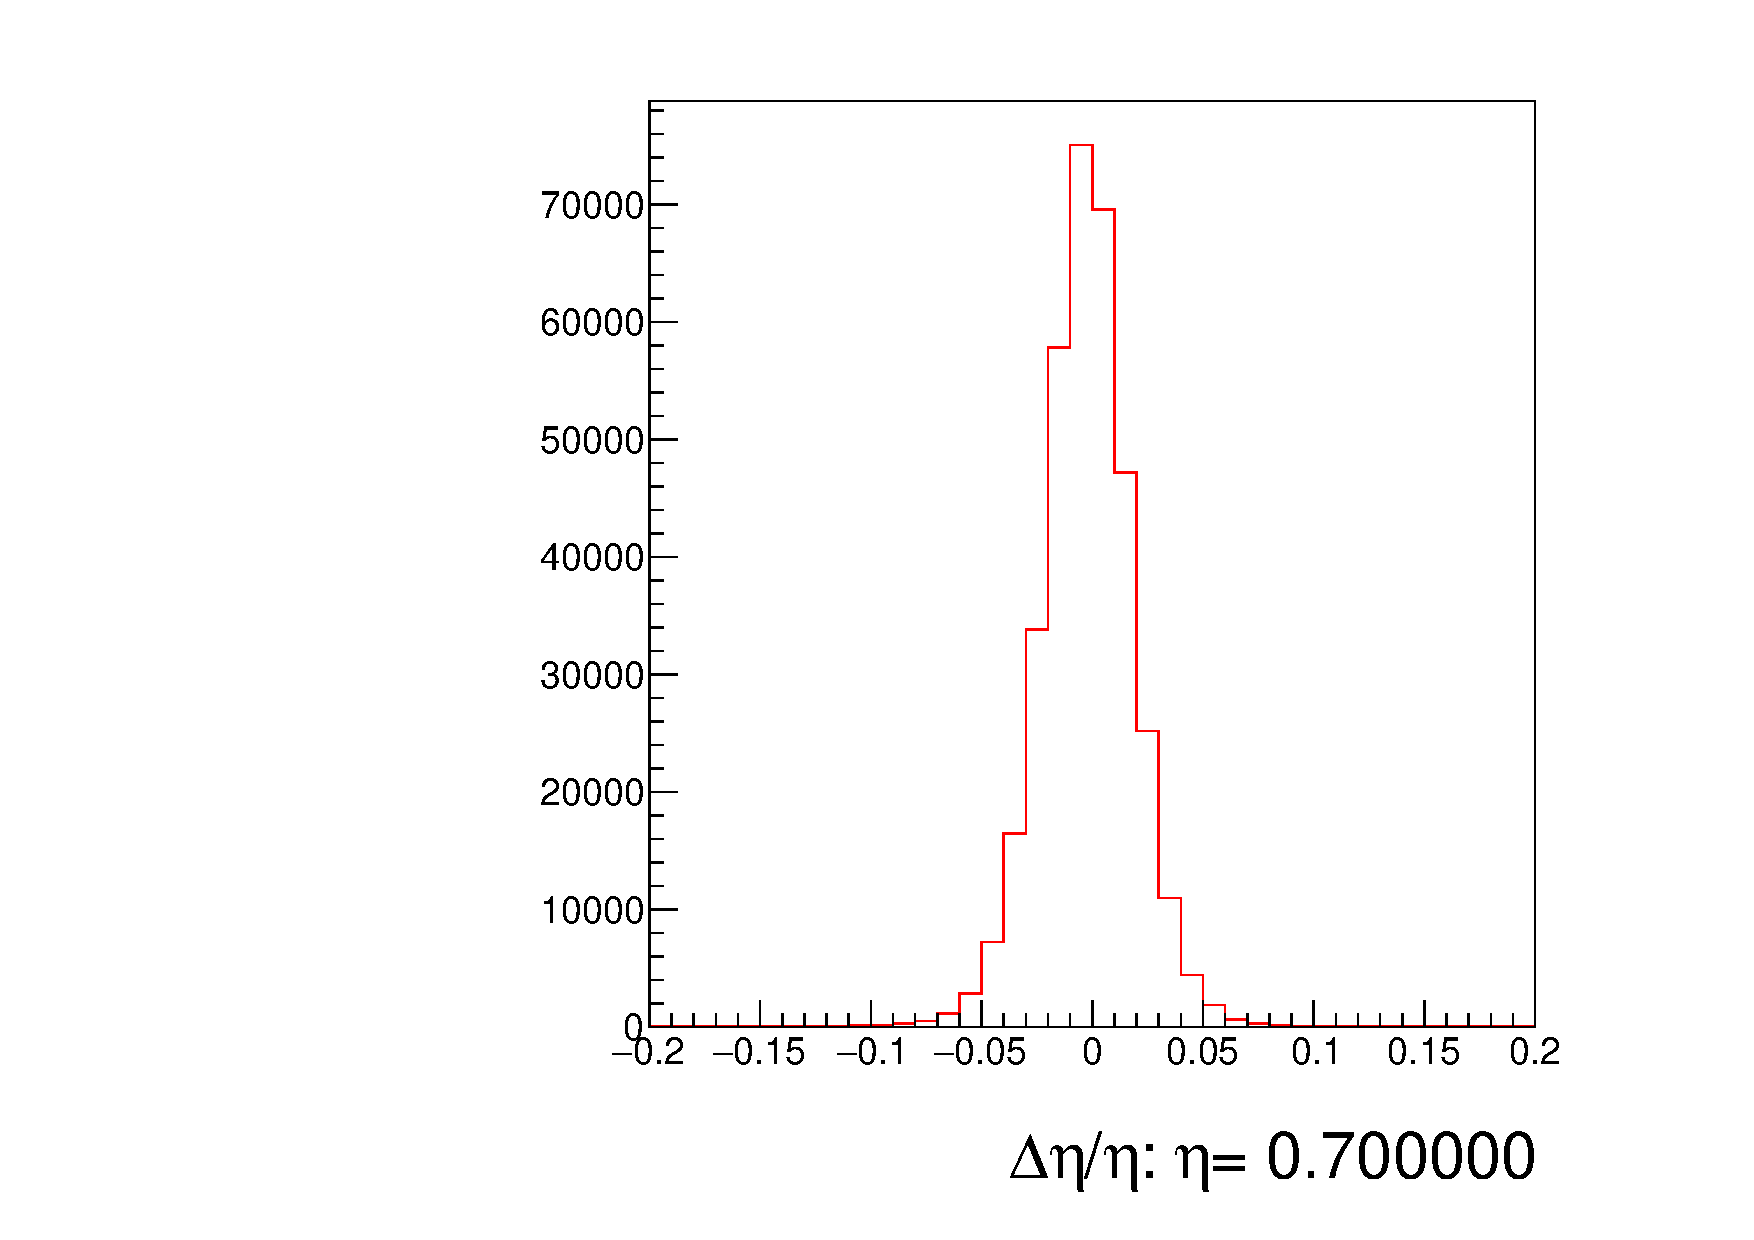
\includegraphics[width=1\linewidth]{Offline_2C_etaRatio_Leading_BJet_eta_lower_Slice}
					\end{minipage}
					\caption{$\Delta \eta_{ratio}$ for the leading \pt $b$-jet with $0 < \eta < 1$ from Data events against $\eta$ of the offline $b$-jet. A slice across the $y$-axis has been taken at $\eta=-1.9$. }
					\label{fig:D:leadingbetacentral}
				\end{figure}
				
				\begin{figure}[h]
					\centering
					
					\begin{minipage}[h]{0.33\linewidth}
						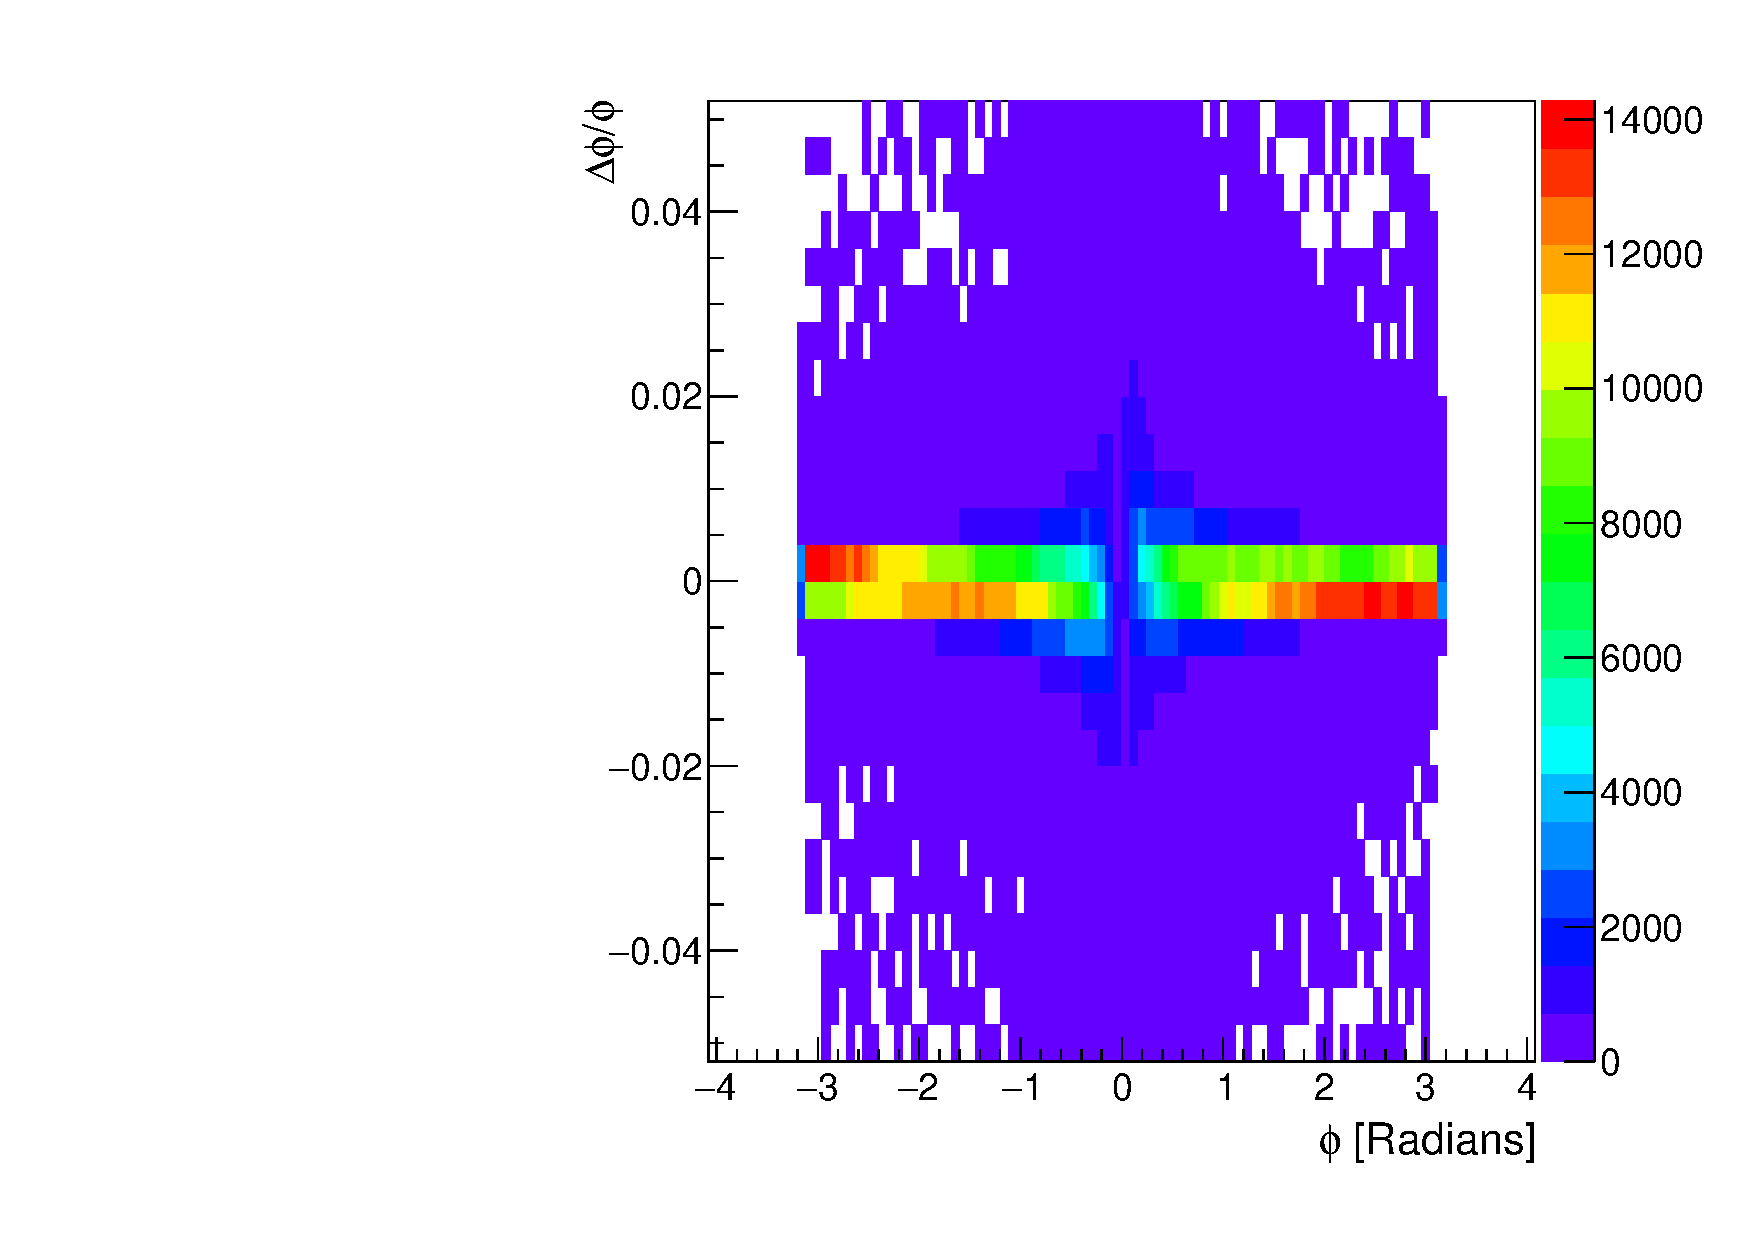
\includegraphics[width=1\linewidth]{Offline_2C_phiRatio_Leading_BJet_eta_lower}
					\end{minipage}
					\quad
					\begin{minipage}[h]{0.33\linewidth}
						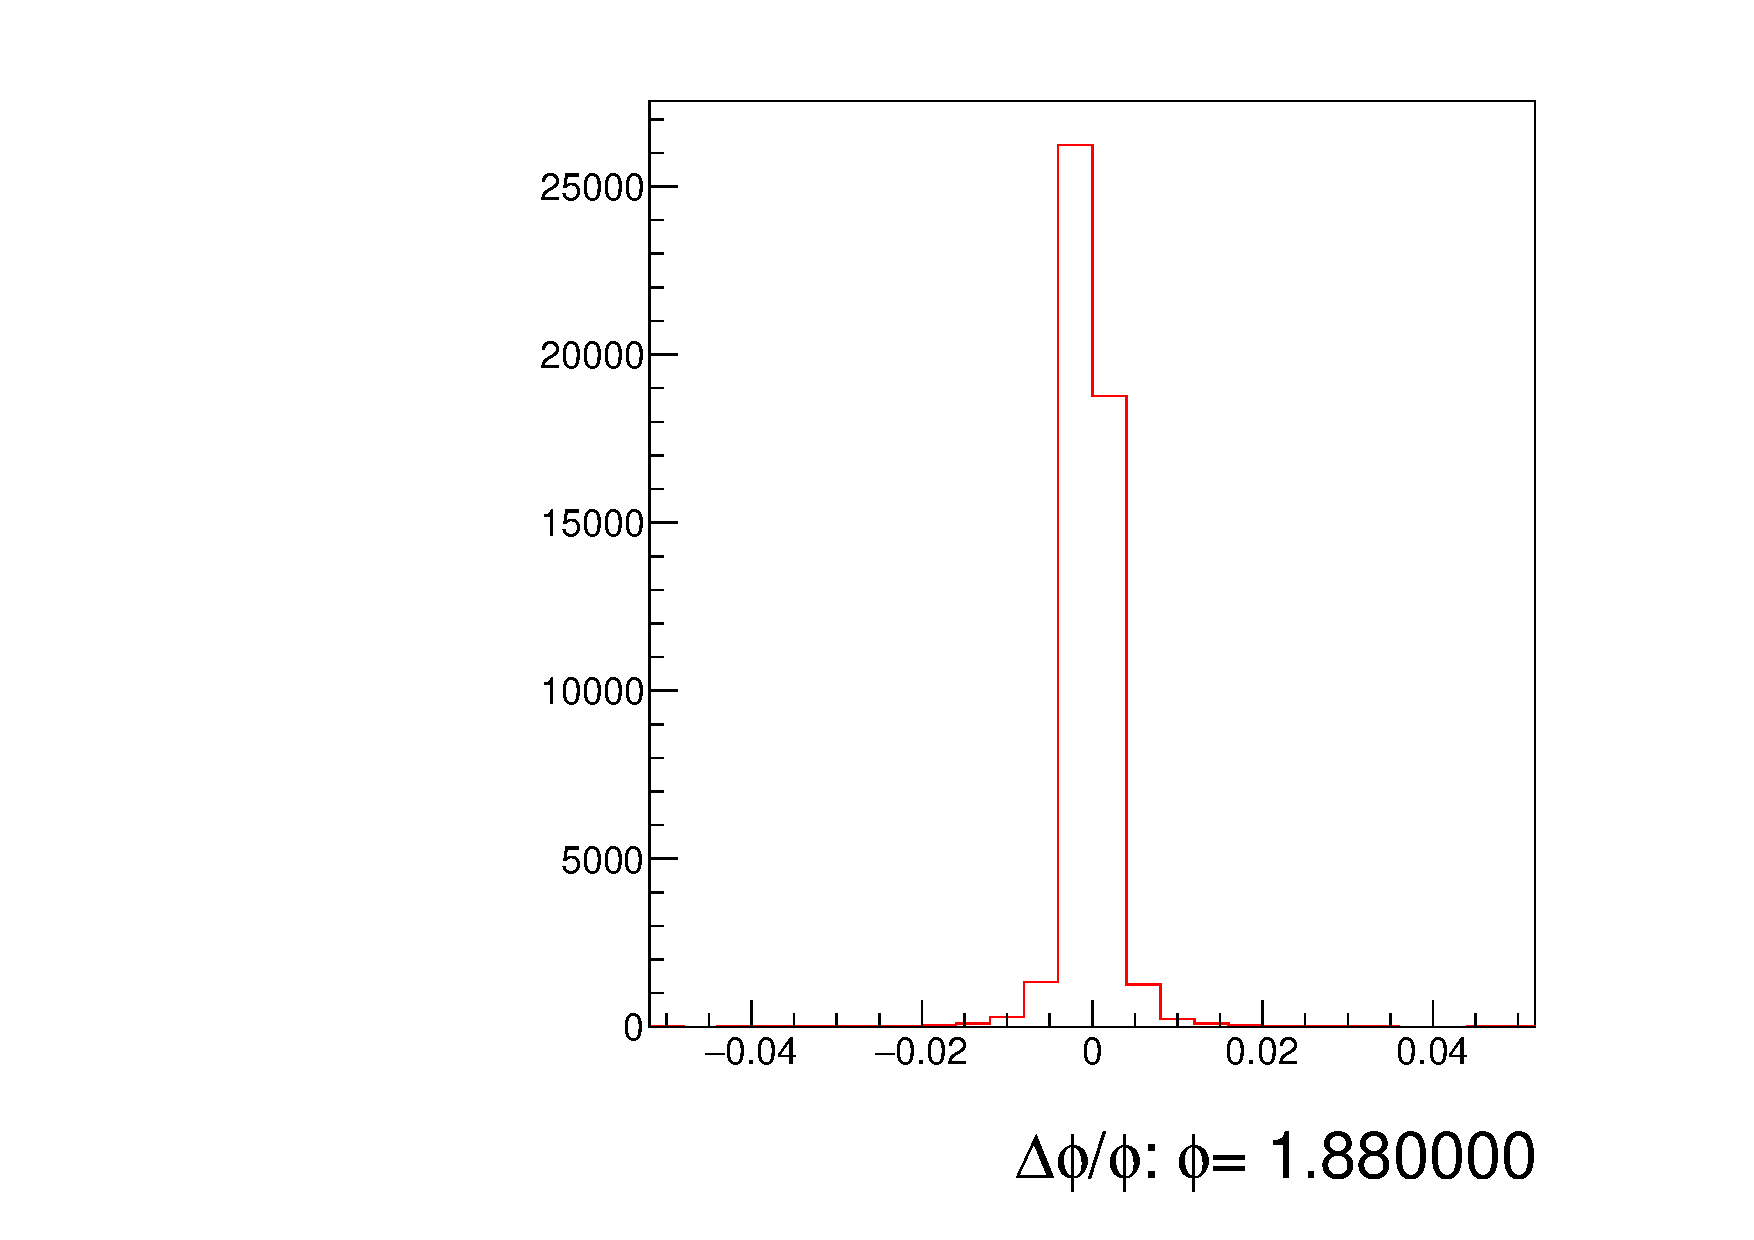
\includegraphics[width=1\linewidth]{Offline_2C_phiRatio_Leading_BJet_eta_lower_Slice}
					\end{minipage}
					\caption{$\Delta \phi_{ratio}$ for the leading \pt $b$-jet with $0 < \eta < 1$ from Data events against $\phi$ of the offline $b$-jet. A slice across the $y$-axis has been taken at $\phi=-1.64$. }
					\label{fig:D:leadingbphicentral}
				\end{figure}
				
				\begin{figure}[h]
					\centering
					
					\begin{minipage}[h]{0.33\linewidth}
						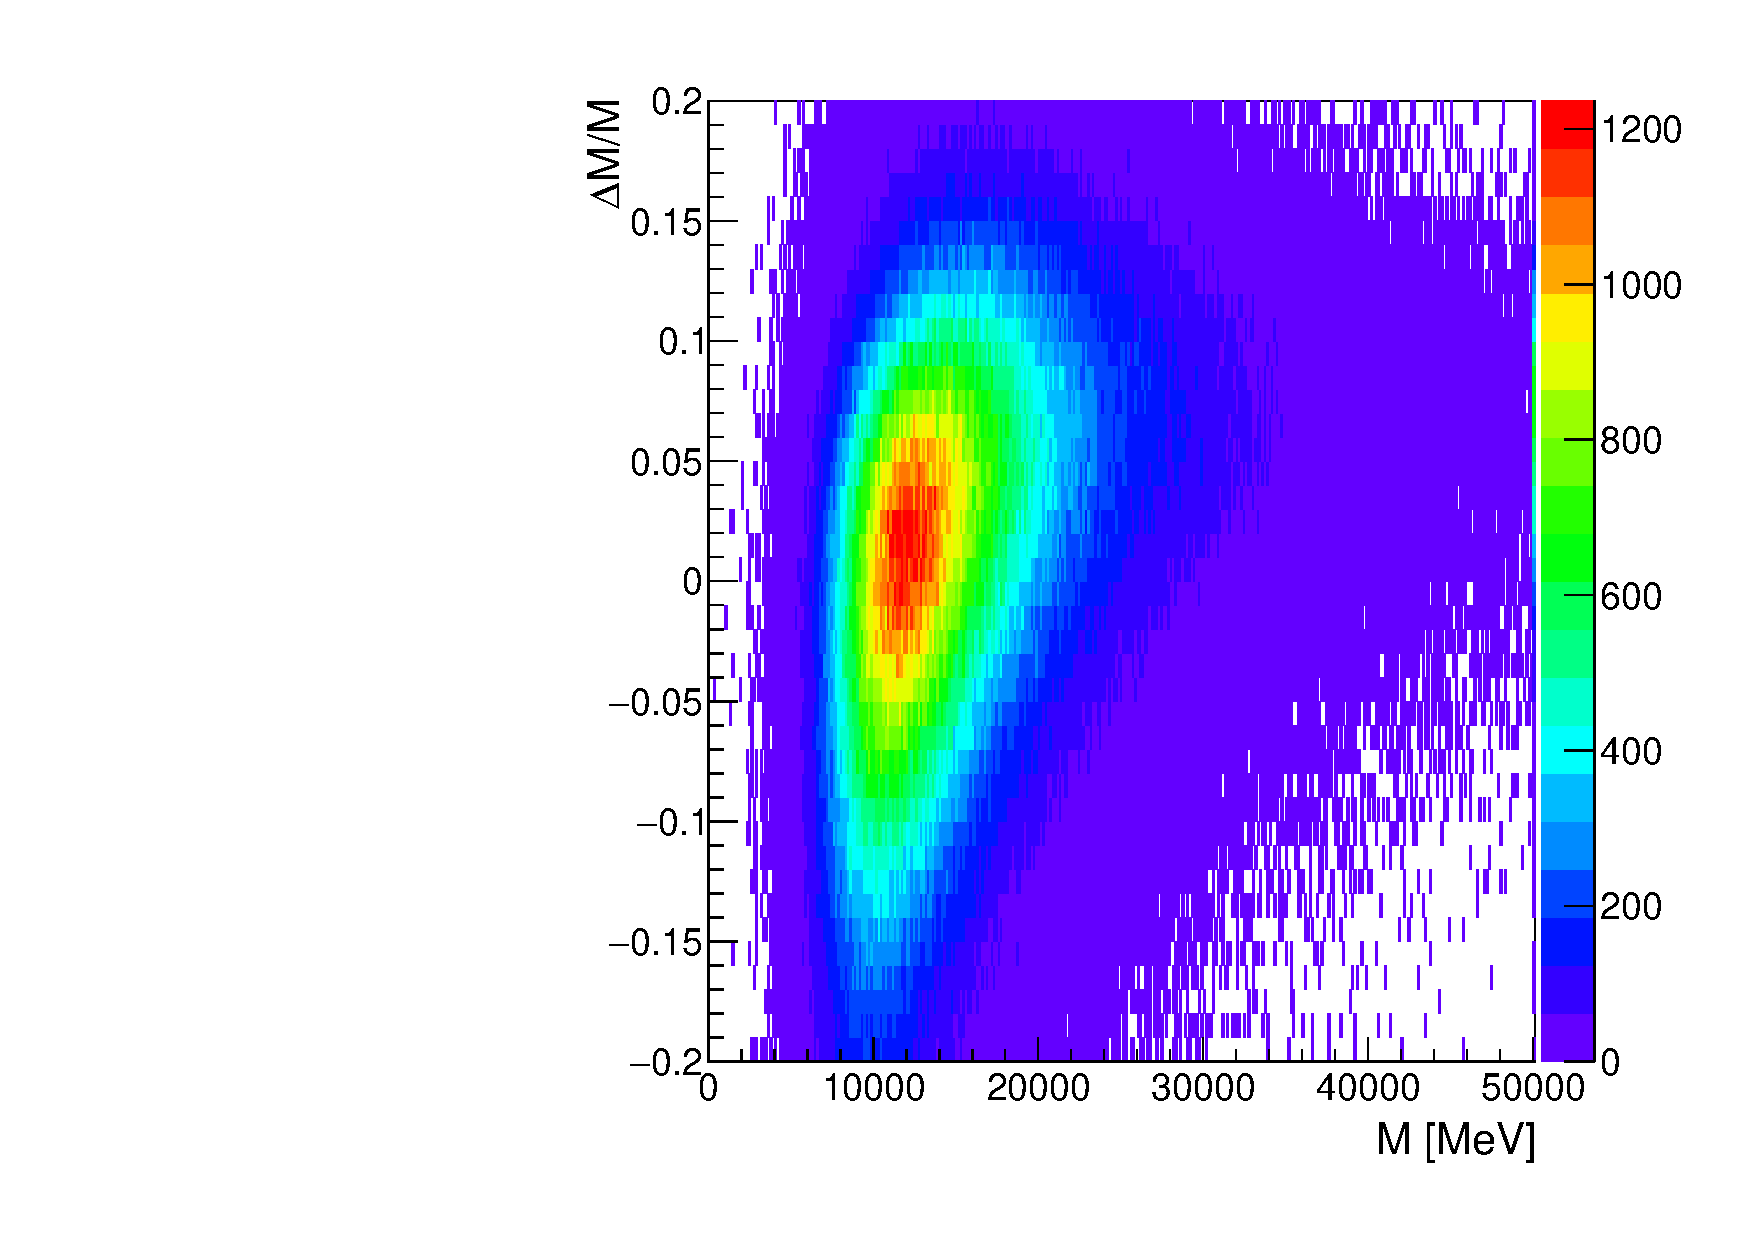
\includegraphics[width=1\linewidth]{Offline_2C_mRatio_Leading_BJet_eta_lower}
					\end{minipage}
					\quad
					\begin{minipage}[h]{0.33\linewidth}
						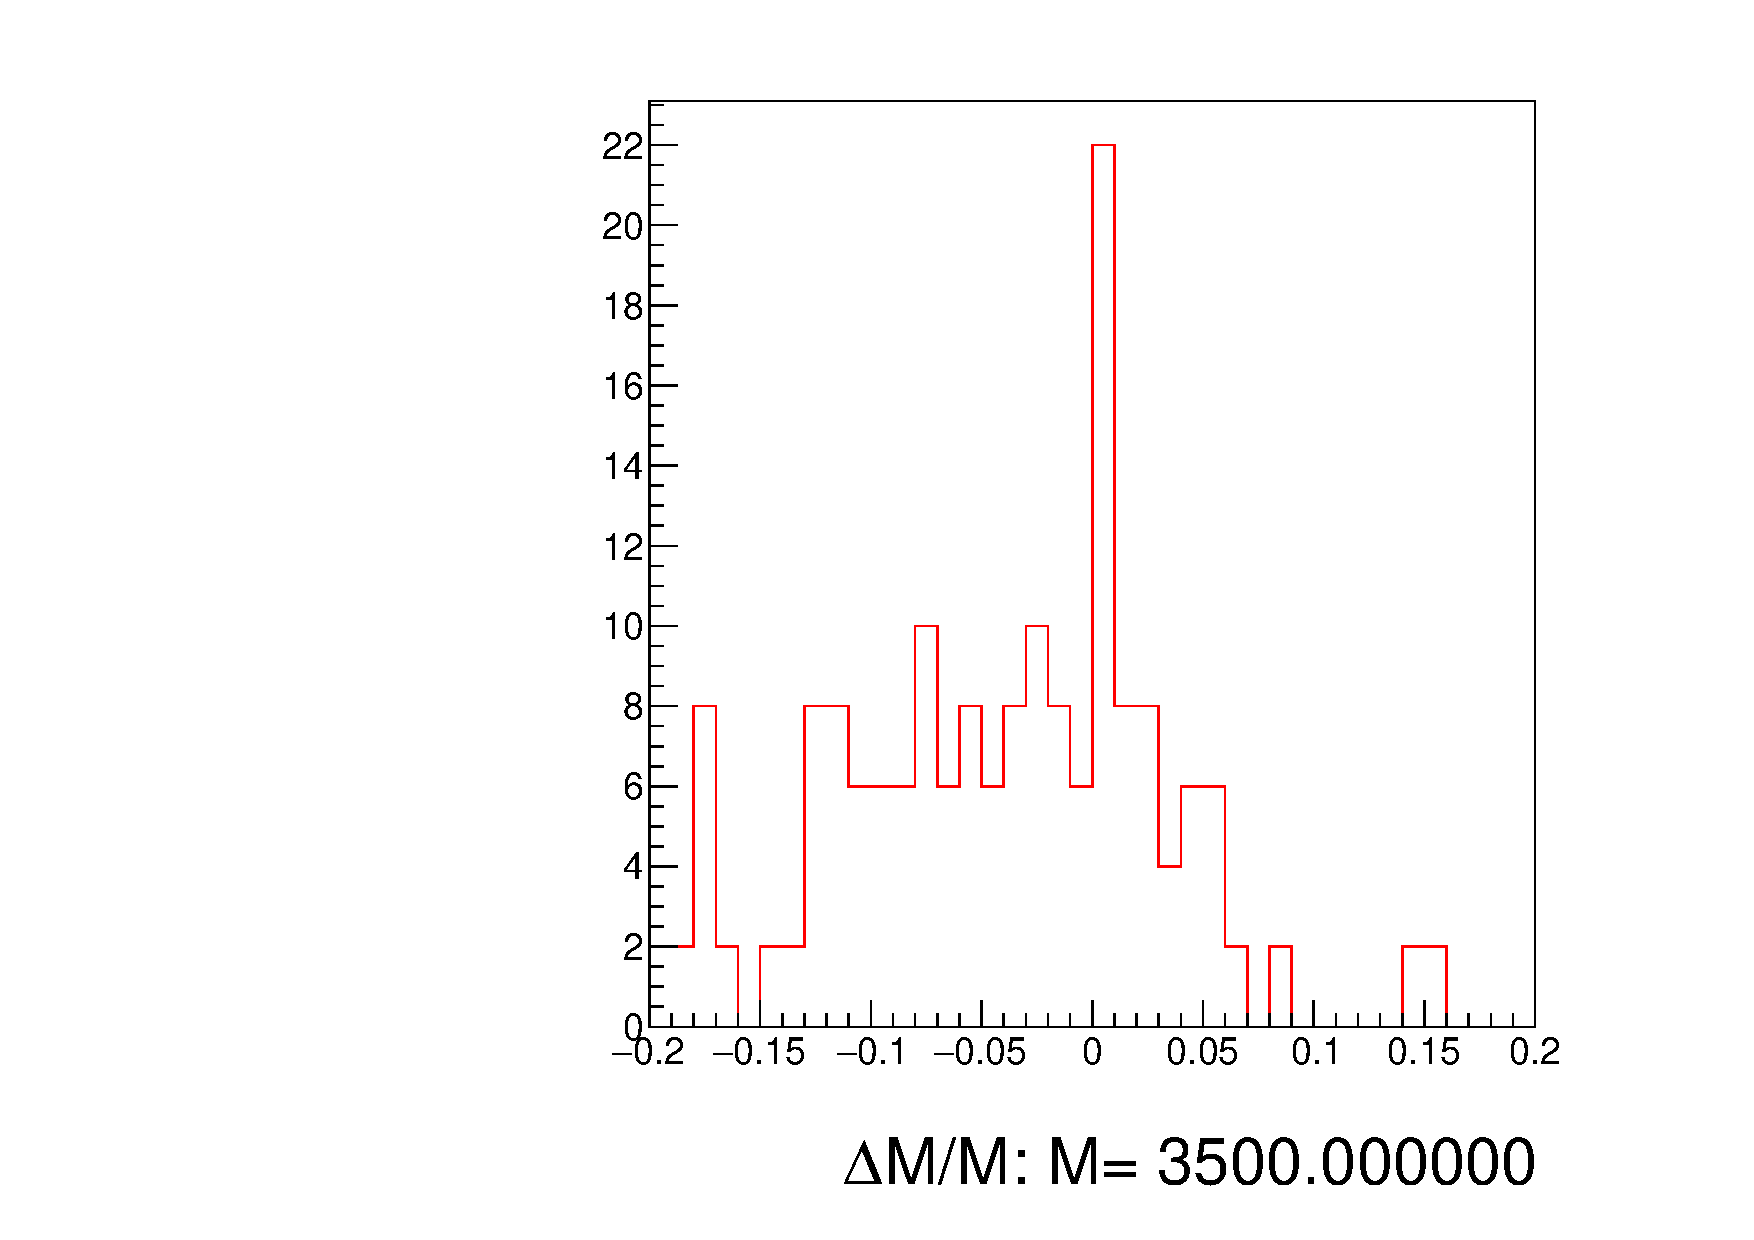
\includegraphics[width=1\linewidth]{Offline_2C_mRatio_Leading_BJet_eta_lower_Slice}
					\end{minipage}
					\caption{$\Delta M_{ratio}$ for the leading \pt $b$-jet with $0 < \eta < 1$ from Data events against $M$ of the offline $b$-jet. A slice across the $y$-axis has been taken at $M=7$GeV. }
					\label{fig:D:leadingbmcentral}
				\end{figure}

\newpage
\subsection{Non b Jets}
		\subsection{Monte-Carlo}

		\begin{figure}[h]
			\centering
			\begin{minipage}[h]{0.33\linewidth}
				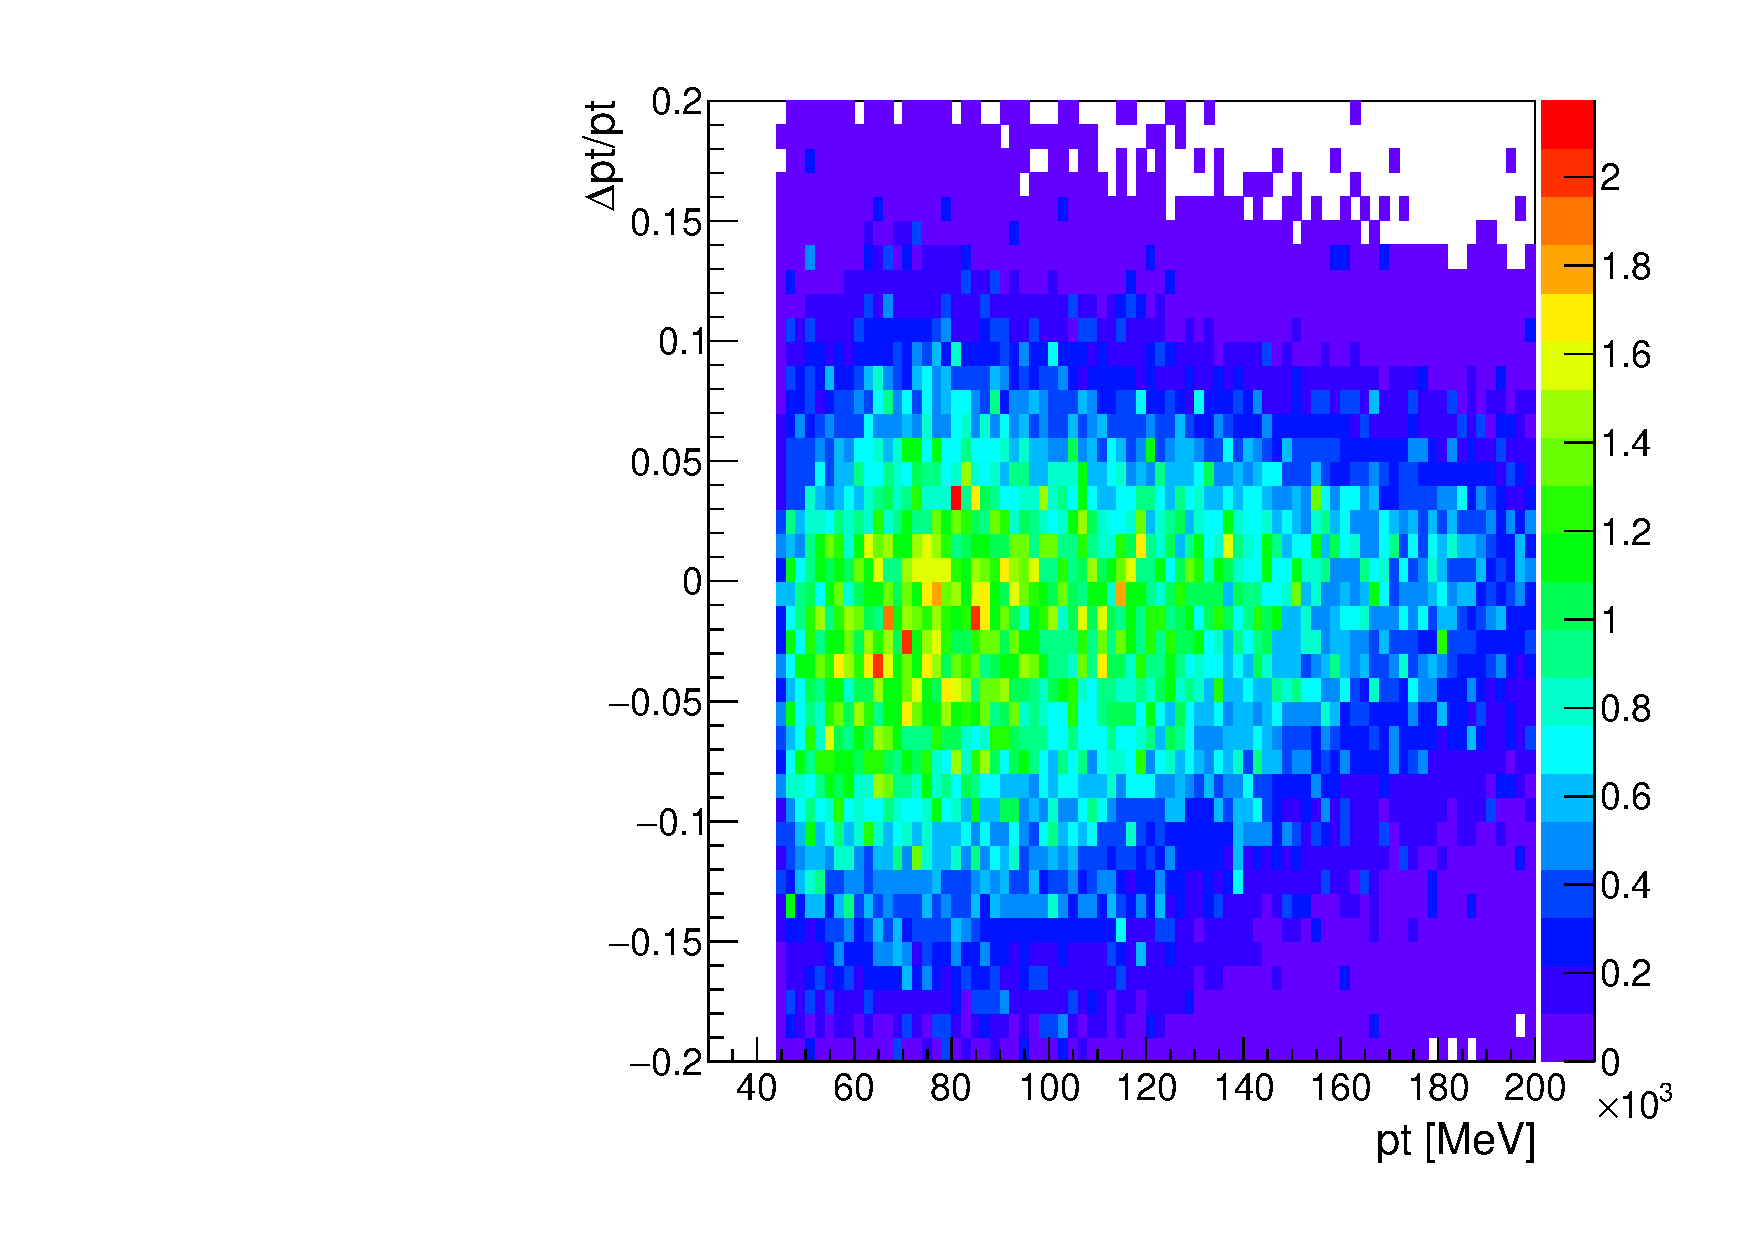
\includegraphics[width=1\linewidth]{ptRatio_Leading_Non_BJet_eta_lower}

			\end{minipage}
			\quad
			\begin{minipage}[h]{0.33\linewidth}
				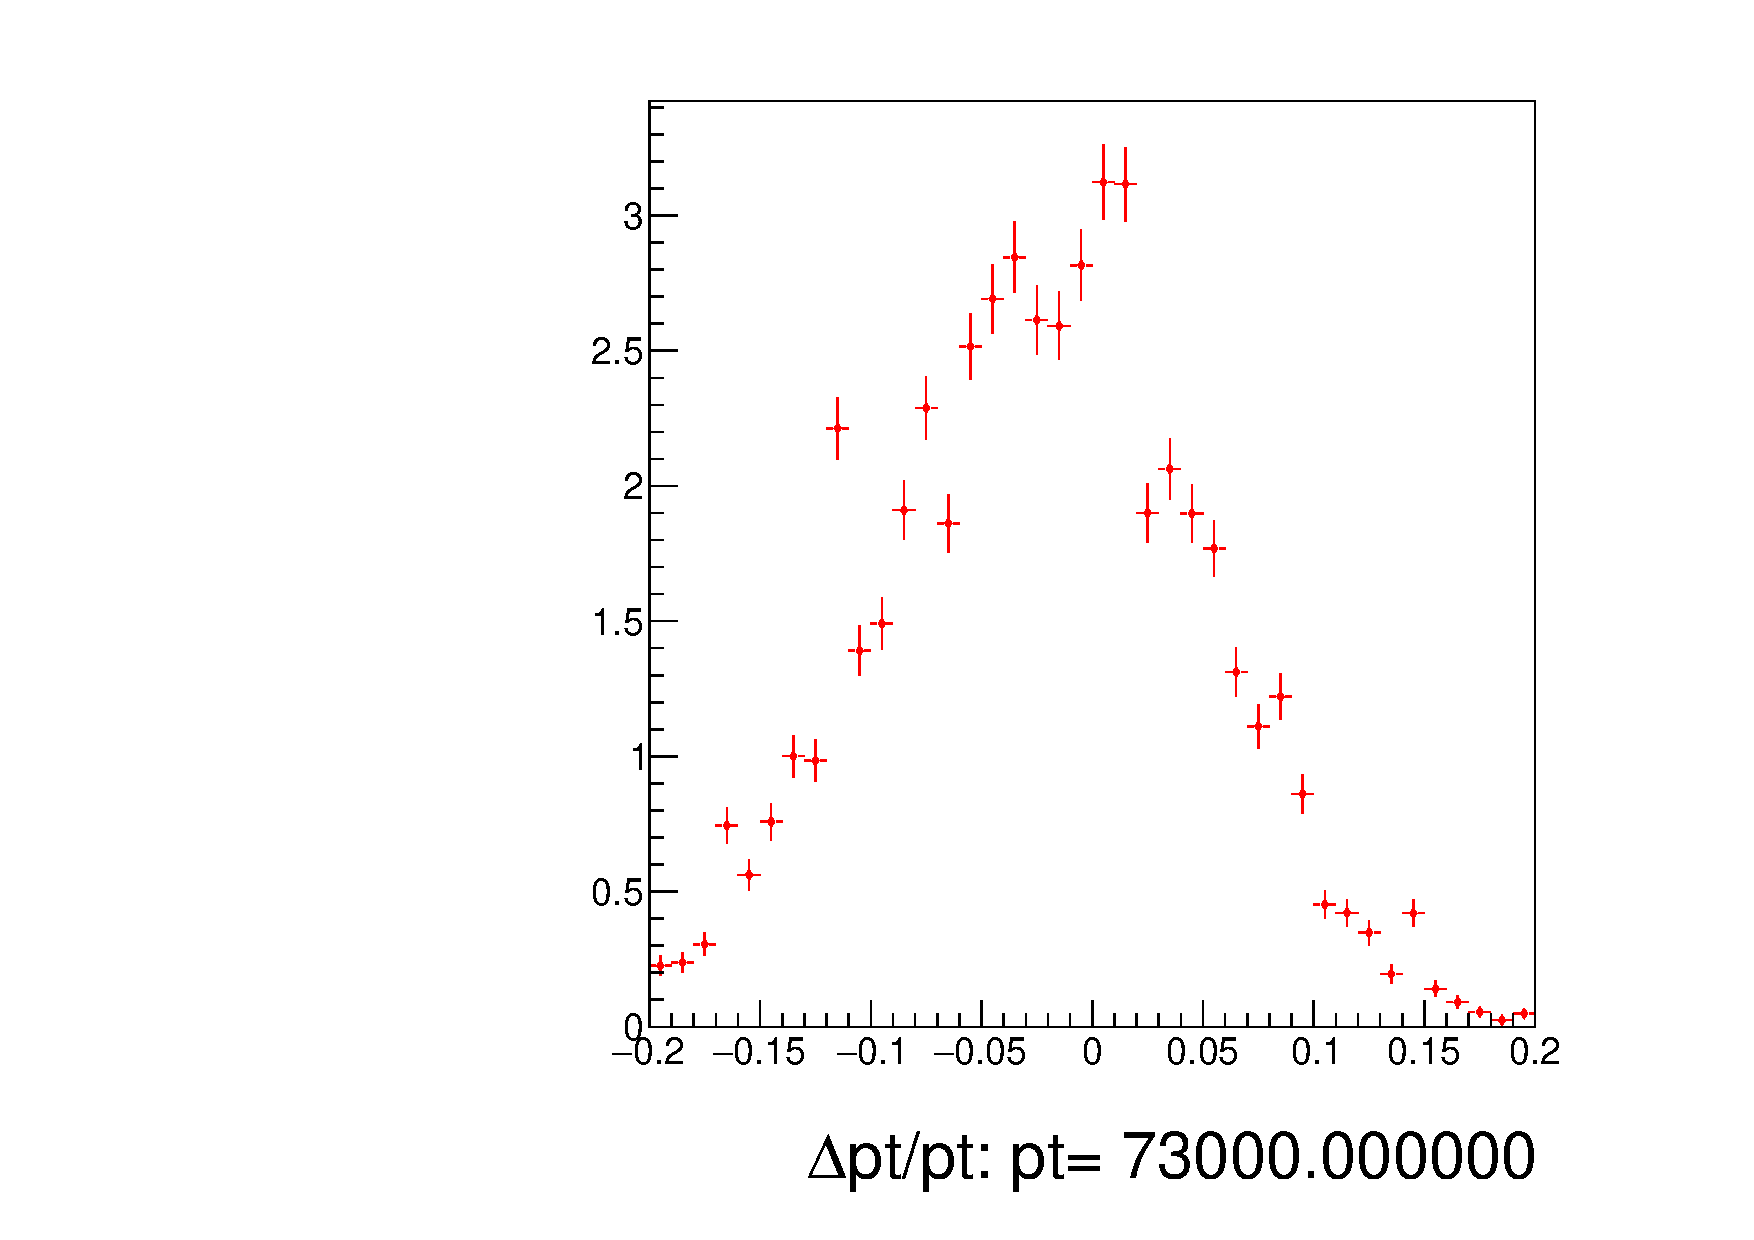
\includegraphics[width=1\linewidth]{ptRatio_Leading_Non_BJet_eta_lower_Slice}
			\end{minipage}
			\caption{$\Delta $\pt$_{ratio}$ for the leading \pt non $b$-jet with $0 < \eta < 1$ from MC events against \pt of the offline $b$-jet. A slice across the $y$-axis has been taken at \pt$=79$GeV. }
			\label{fig:MC:leadingnonbptcentral}
		\end{figure}

		\begin{figure}[h]
			\centering

			\begin{minipage}[h]{0.33\linewidth}
				\includegraphics[width=1\linewidth]{etaRatio_Leading_Non_BJet_eta_lower}
			\end{minipage}
			\quad
			\begin{minipage}[h]{0.33\linewidth}
				\includegraphics[width=1\linewidth]{etaRatio_Leading_Non_BJet_eta_lower_Slice}
			\end{minipage}
			\caption{$\Delta \eta_{ratio}$ for the leading \pt non $b$-jet with $0 < \eta < 1$ from MC events against $\eta$ of the offline $b$-jet. A slice across the $y$-axis has been taken at $\eta=-1.9$. }
			\label{fig:MC:leadingnonbetacentral}
		\end{figure}

		\begin{figure}[h]
			\centering

			\begin{minipage}[h]{0.33\linewidth}
				\includegraphics[width=1\linewidth]{phiRatio_Leading_Non_BJet_eta_lower}
			\end{minipage}
			\quad
			\begin{minipage}[h]{0.33\linewidth}
				\includegraphics[width=1\linewidth]{phiRatio_Leading_Non_BJet_eta_lower_Slice}
			\end{minipage}
			\caption{$\Delta \phi_{ratio}$ for the leading \pt non $b$-jet with $0 < \eta < 1$ from MC events against $\phi$ of the offline $b$-jet. A slice across the $y$-axis has been taken at $\phi=-1.64$. }
			\label{fig:MC:leadingnonbphicentral}
		\end{figure}

		\begin{figure}[h]
			\centering

			\begin{minipage}[h]{0.33\linewidth}
				\includegraphics[width=1\linewidth]{mRatio_Leading_Non_BJet_eta_lower}
			\end{minipage}
			\quad
			\begin{minipage}[h]{0.33\linewidth}
				\includegraphics[width=1\linewidth]{mRatio_Leading_Non_BJet_eta_lower_Slice}
			\end{minipage}
			\caption{$\Delta M_{ratio}$ for the leading \pt non $b$-jet with $0 < \eta < 1$ from MC events against $M$ of the offline $b$-jet. A slice across the $y$-axis has been taken at $M=7$GeV. }
			\label{fig:MC:leadingnonbmcentral}
		\end{figure}

\newpage
		\subsection{Data}
		
		
		\begin{figure}[h]
			\centering
			\begin{minipage}[h]{0.33\linewidth}
				\includegraphics[width=1\linewidth]{Offline_2C_ptRatio_Leading_Non_BJet_eta_lower}
				
			\end{minipage}
			\quad
			\begin{minipage}[h]{0.33\linewidth}
				\includegraphics[width=1\linewidth]{Offline_2C_ptRatio_Leading_Non_BJet_eta_lower_Slice}
			\end{minipage}
			\caption{$\Delta $\pt$_{ratio}$ for the leading \pt non $b$-jet with $0 < \eta < 1$ from Data events against \pt of the offline $b$-jet. A slice across the $y$-axis has been taken at \pt$=79$GeV. }
			\label{fig:D:leadingnonbptcentral}
		\end{figure}
		
		\begin{figure}[h]
			\centering
			
			\begin{minipage}[h]{0.33\linewidth}
				\includegraphics[width=1\linewidth]{Offline_2C_etaRatio_Leading_Non_BJet_eta_lower}
			\end{minipage}
			\quad
			\begin{minipage}[h]{0.33\linewidth}
				\includegraphics[width=1\linewidth]{Offline_2C_etaRatio_Leading_Non_BJet_eta_lower_Slice}
			\end{minipage}
			\caption{$\Delta \eta_{ratio}$ for the leading \pt non $b$-jet with $0 < \eta < 1$ from Data events against $\eta$ of the offline $b$-jet. A slice across the $y$-axis has been taken at $\eta=-1.9$. }
			\label{fig:D:leadingnonbetacentral}
		\end{figure}
		
		\begin{figure}[h]
			\centering
			
			\begin{minipage}[h]{0.33\linewidth}
				\includegraphics[width=1\linewidth]{Offline_2C_phiRatio_Leading_Non_BJet_eta_lower}
			\end{minipage}
			\quad
			\begin{minipage}[h]{0.33\linewidth}
				\includegraphics[width=1\linewidth]{Offline_2C_phiRatio_Leading_Non_BJet_eta_lower_Slice}
			\end{minipage}
			\caption{$\Delta \phi_{ratio}$ for the leading \pt non $b$-jet with $0 < \eta < 1$ from Data events against $\phi$ of the offline $b$-jet. A slice across the $y$-axis has been taken at $\phi=-1.64$. }
			\label{fig:D:leadingnonbphicentral}
		\end{figure}
		
		\begin{figure}[h]
			\centering
			
			\begin{minipage}[h]{0.33\linewidth}
				\includegraphics[width=1\linewidth]{Offline_2C_mRatio_Leading_Non_BJet_eta_lower}
			\end{minipage}
			\quad
			\begin{minipage}[h]{0.33\linewidth}
				\includegraphics[width=1\linewidth]{Offline_2C_mRatio_Leading_Non_BJet_eta_lower_Slice}
			\end{minipage}
			\caption{$\Delta M_{ratio}$ for the leading \pt non $b$-jet with $0 < \eta < 1$ from Data events against $M$ of the offline $b$-jet. A slice across the $y$-axis has been taken at $M=7$GeV. }
			\label{fig:D:leadingnonbmcentral}
		\end{figure}

\newpage\newpage
\section{Core}

	\subsection{Monte-Carlo}

	\begin{figure}[h]
		\centering
		\begin{minipage}[h]{0.33\linewidth}
			\includegraphics[width=1\linewidth]{ptRatio_Leading_BJet_eta_signal}

		\end{minipage}
		\quad
		\begin{minipage}[h]{0.33\linewidth}
			\includegraphics[width=1\linewidth]{ptRatio_Leading_BJet_eta_signal_Slice}
		\end{minipage}
		\caption{$\Delta $\pt$_{ratio}$ for the leading \pt $b$-jet with $1 < \eta < 2.4$ from MC events against \pt of the offline $b$-jet. A slice across the $y$-axis has been taken at \pt$=79$GeV. }
		\label{fig:MC:leadingbptcore}
	\end{figure}

	\begin{figure}[h]
		\centering

		\begin{minipage}[h]{0.33\linewidth}
			\includegraphics[width=1\linewidth]{etaRatio_Leading_BJet_eta_signal}
		\end{minipage}
		\quad
		\begin{minipage}[h]{0.33\linewidth}
			\includegraphics[width=1\linewidth]{etaRatio_Leading_BJet_eta_signal_Slice}
		\end{minipage}
		\caption{$\Delta \eta_{ratio}$ for the leading \pt $b$-jet with $1 < \eta < 2.4$ from MC events against $\eta$ of the offline $b$-jet. A slice across the $y$-axis has been taken at $\eta=-1.9$. }
		\label{fig:MC:leadingbetacore}
	\end{figure}

	\begin{figure}[h]
		\centering

		\begin{minipage}[h]{0.33\linewidth}
			\includegraphics[width=1\linewidth]{phiRatio_Leading_BJet_eta_signal}
		\end{minipage}
		\quad
		\begin{minipage}[h]{0.33\linewidth}
			\includegraphics[width=1\linewidth]{phiRatio_Leading_BJet_eta_signal_Slice}
		\end{minipage}
		\caption{$\Delta \phi_{ratio}$ for the leading \pt $b$-jet with $1 < \eta < 2.4$ from MC events against $\phi$ of the offline $b$-jet. A slice across the $y$-axis has been taken at $\phi=-1.64$. }
		\label{fig:MC:leadingbphicore}
	\end{figure}

	\begin{figure}[h]
		\centering

		\begin{minipage}[h]{0.33\linewidth}
			\includegraphics[width=1\linewidth]{mRatio_Leading_BJet_eta_signal}
		\end{minipage}
		\quad
		\begin{minipage}[h]{0.33\linewidth}
			\includegraphics[width=1\linewidth]{mRatio_Leading_BJet_eta_signal_Slice}
		\end{minipage}
		\caption{$\Delta M_{ratio}$ for the leading \pt $b$-jet with $1 < \eta < 2.4$ from MC events against $M$ of the offline $b$-jet. A slice across the $y$-axis has been taken at $M=7$GeV. }
		\label{fig:MC:leadingbmcore}
	\end{figure}

\newpage
	\subsubsection{Data}
	
		\begin{figure}[h]
			\centering
			\begin{minipage}[h]{0.33\linewidth}
				\includegraphics[width=1\linewidth]{Offline_2C_ptRatio_Leading_BJet_eta_signal}
				
			\end{minipage}
			\quad
			\begin{minipage}[h]{0.33\linewidth}
				\includegraphics[width=1\linewidth]{Offline_2C_ptRatio_Leading_BJet_eta_signal_Slice}
			\end{minipage}
			\caption{$\Delta $\pt$_{ratio}$ for the leading \pt $b$-jet with $1 < \eta < 2.4$ from Data events against \pt of the offline $b$-jet. A slice across the $y$-axis has been taken at \pt$=79$GeV. }
			\label{fig:D:leadingbptcore}
		\end{figure}
		
		\begin{figure}[h]
			\centering
			
			\begin{minipage}[h]{0.33\linewidth}
				\includegraphics[width=1\linewidth]{Offline_2C_etaRatio_Leading_BJet_eta_signal}
			\end{minipage}
			\quad
			\begin{minipage}[h]{0.33\linewidth}
				\includegraphics[width=1\linewidth]{Offline_2C_etaRatio_Leading_BJet_eta_signal_Slice}
			\end{minipage}
			\caption{$\Delta \eta_{ratio}$ for the leading \pt $b$-jet with $1 < \eta < 2.4$ from Data events against $\eta$ of the offline $b$-jet. A slice across the $y$-axis has been taken at $\eta=-1.9$. }
			\label{fig:D:leadingbetacore}
		\end{figure}
		
		\begin{figure}[h]
			\centering
			
			\begin{minipage}[h]{0.33\linewidth}
				\includegraphics[width=1\linewidth]{Offline_2C_phiRatio_Leading_BJet_eta_signal}
			\end{minipage}
			\quad
			\begin{minipage}[h]{0.33\linewidth}
				\includegraphics[width=1\linewidth]{Offline_2C_phiRatio_Leading_BJet_eta_signal_Slice}
			\end{minipage}
			\caption{$\Delta \phi_{ratio}$ for the leading \pt $b$-jet with $1 < \eta < 2.4$ from Data events against $\phi$ of the offline $b$-jet. A slice across the $y$-axis has been taken at $\phi=-1.64$. }
			\label{fig:D:leadingbphicore}
		\end{figure}
		
		\begin{figure}[h]
			\centering
			
			\begin{minipage}[h]{0.33\linewidth}
				\includegraphics[width=1\linewidth]{Offline_2C_mRatio_Leading_BJet_eta_signal}
			\end{minipage}
			\quad
			\begin{minipage}[h]{0.33\linewidth}
				\includegraphics[width=1\linewidth]{Offline_2C_mRatio_Leading_BJet_eta_signal_Slice}
			\end{minipage}
			\caption{$\Delta M_{ratio}$ for the leading \pt $b$-jet with $1 < \eta < 2.4$ from Data events against $M$ of the offline $b$-jet. A slice across the $y$-axis has been taken at $M=7$GeV. }
			\label{fig:D:leadingbmcore}
		\end{figure}

\newpage
	\subsection{Non Bjets}

	\subsection{Monte-Carlo}

	\begin{figure}[h]
		\centering
		\begin{minipage}[h]{0.33\linewidth}
			\includegraphics[width=1\linewidth]{ptRatio_Leading_Non_BJet_eta_signal}

		\end{minipage}
		\quad
		\begin{minipage}[h]{0.33\linewidth}
			\includegraphics[width=1\linewidth]{ptRatio_Leading_Non_BJet_eta_signal_Slice}
		\end{minipage}
		\caption{$\Delta $\pt$_{ratio}$ for the leading \pt non $b$-jet with $1 < \eta < 2.4$ from MC events against \pt of the offline $b$-jet. A slice across the $y$-axis has been taken at \pt$=79$GeV. }
		\label{fig:MC:leadingnonbptcore}
	\end{figure}

	\begin{figure}[h]
		\centering

		\begin{minipage}[h]{0.33\linewidth}
			\includegraphics[width=1\linewidth]{etaRatio_Leading_Non_BJet_eta_signal}
		\end{minipage}
		\quad
		\begin{minipage}[h]{0.33\linewidth}
			\includegraphics[width=1\linewidth]{etaRatio_Leading_Non_BJet_eta_signal_Slice}
		\end{minipage}
		\caption{$\Delta \eta_{ratio}$ for the leading \pt non $b$-jet with $1 < \eta < 2.4$ from MC events against $\eta$ of the offline $b$-jet. A slice across the $y$-axis has been taken at $\eta=-1.9$. }
		\label{fig:MC:leadingnonbetacore}
	\end{figure}

	\begin{figure}[h]
		\centering

		\begin{minipage}[h]{0.33\linewidth}
			\includegraphics[width=1\linewidth]{phiRatio_Leading_Non_BJet_eta_signal}
		\end{minipage}
		\quad
		\begin{minipage}[h]{0.33\linewidth}
			\includegraphics[width=1\linewidth]{phiRatio_Leading_Non_BJet_eta_signal_Slice}
		\end{minipage}
		\caption{$\Delta \phi_{ratio}$ for the leading \pt non $b$-jet with $1 < \eta < 2.4$\textbf{} from MC events against $\phi$ of the offline $b$-jet. A slice across the $y$-axis has been taken at $\phi=-1.64$. }
		\label{fig:MC:leadingnonbphicore}
	\end{figure}

	\begin{figure}[h]
		\centering

		\begin{minipage}[h]{0.33\linewidth}
			\includegraphics[width=1\linewidth]{mRatio_Leading_Non_BJet_eta_signal}
		\end{minipage}
		\quad
		\begin{minipage}[h]{0.33\linewidth}
			\includegraphics[width=1\linewidth]{mRatio_Leading_Non_BJet_eta_signal_Slice}
		\end{minipage}
		\caption{$\Delta M_{ratio}$ for the leading \pt non $b$-jet with $1 < \eta < 2.4$ from MC events against $M$ of the offline $b$-jet. A slice across the $y$-axis has been taken at $M=7$GeV. }
		\label{fig:MC:leadingnonbmcore}
	\end{figure}
	
	\newpage
	\subsection{Data}
	
		\begin{figure}[h]
			\centering
			\begin{minipage}[h]{0.33\linewidth}
				\includegraphics[width=1\linewidth]{Offline_2C_ptRatio_Leading_Non_BJet_eta_signal}
				
			\end{minipage}
			\quad
			\begin{minipage}[h]{0.33\linewidth}
				\includegraphics[width=1\linewidth]{Offline_2C_ptRatio_Leading_Non_BJet_eta_signal_Slice}
			\end{minipage}
			\caption{$\Delta $\pt$_{ratio}$ for the leading \pt non $b$-jet with $1 < \eta < 2.4$ from Data events against \pt of the offline $b$-jet. A slice across the $y$-axis has been taken at \pt$=79$GeV. }
			\label{fig:D:leadingnonbptcore}
		\end{figure}
		
		\begin{figure}[h]
			\centering
			
			\begin{minipage}[h]{0.33\linewidth}
				\includegraphics[width=1\linewidth]{Offline_2C_etaRatio_Leading_Non_BJet_eta_signal}
			\end{minipage}
			\quad
			\begin{minipage}[h]{0.33\linewidth}
				\includegraphics[width=1\linewidth]{Offline_2C_etaRatio_Leading_Non_BJet_eta_signal_Slice}
			\end{minipage}
			\caption{$\Delta \eta_{ratio}$ for the leading \pt non $b$-jet with $1 < \eta < 2.4$ from Data events against $\eta$ of the offline $b$-jet. A slice across the $y$-axis has been taken at $\eta=-1.9$. }
			\label{fig:D:leadingnonbetacore}
		\end{figure}
		
		\begin{figure}[h]
			\centering
			
			\begin{minipage}[h]{0.33\linewidth}
				\includegraphics[width=1\linewidth]{Offline_2C_phiRatio_Leading_Non_BJet_eta_signal}
			\end{minipage}
			\quad
			\begin{minipage}[h]{0.33\linewidth}
				\includegraphics[width=1\linewidth]{Offline_2C_phiRatio_Leading_Non_BJet_eta_signal_Slice}
			\end{minipage}
			\caption{$\Delta \phi_{ratio}$ for the leading \pt non $b$-jet with $1 < \eta < 2.4$\textbf{} from Data events against $\phi$ of the offline $b$-jet. A slice across the $y$-axis has been taken at $\phi=-1.64$. }
			\label{fig:D:leadingnonbphicore}
		\end{figure}
		
		\begin{figure}[h]
			\centering
			
			\begin{minipage}[h]{0.33\linewidth}
				\includegraphics[width=1\linewidth]{Offline_2C_mRatio_Leading_Non_BJet_eta_signal}
			\end{minipage}
			\quad
			\begin{minipage}[h]{0.33\linewidth}
				\includegraphics[width=1\linewidth]{Offline_2C_mRatio_Leading_Non_BJet_eta_signal_Slice}
			\end{minipage}
			\caption{$\Delta M_{ratio}$ for the leading \pt non $b$-jet with $1 < \eta < 2.4$ from Data events against $M$ of the offline $b$-jet. A slice across the $y$-axis has been taken at $M=7$GeV. }
			\label{fig:D:leadingnonbmcore}
		\end{figure}
		
		

\newpage spacing\newpage spacing \newpage
\section{Forward  Jets}

		\subsection{Monte-Carlo}

		\begin{figure}[h]
			\centering
			\begin{minipage}[h]{0.33\linewidth}
				\includegraphics[width=1\linewidth]{ptRatio_Leading_BJet_eta_upper}

			\end{minipage}
			\quad
			\begin{minipage}[h]{0.33\linewidth}
				\includegraphics[width=1\linewidth]{ptRatio_Leading_BJet_eta_upper_Slice}
			\end{minipage}
			\caption{$\Delta $\pt$_{ratio}$ for the leading \pt $b$-jet with $2.4 < |\eta|$ from MC events against \pt of the offline $b$-jet. A slice across the $y$-axis has been taken at \pt$=79$GeV. }
			\label{fig:MC:leadingbptforward}
		\end{figure}

		\begin{figure}[h]
			\centering

			\begin{minipage}[h]{0.33\linewidth}
				\includegraphics[width=1\linewidth]{etaRatio_Leading_BJet_eta_upper}
			\end{minipage}
			\quad
			\begin{minipage}[h]{0.33\linewidth}
				\includegraphics[width=1\linewidth]{etaRatio_Leading_BJet_eta_upper_Slice}
			\end{minipage}
			\caption{$\Delta \eta_{ratio}$ for the leading \pt $b$-jet $2.4 < |\eta|$ from MC events against $\eta$ of the offline $b$-jet. A slice across the $y$-axis has been taken at $\eta=-1.9$. }
			\label{fig:MC:leadingbetaforward}
		\end{figure}

		\begin{figure}[h]
			\centering

			\begin{minipage}[h]{0.33\linewidth}
				\includegraphics[width=1\linewidth]{phiRatio_Leading_BJet_eta_upper}
			\end{minipage}
			\quad
			\begin{minipage}[h]{0.33\linewidth}
				\includegraphics[width=1\linewidth]{phiRatio_Leading_BJet_eta_upper_Slice}
			\end{minipage}
			\caption{$\Delta \phi_{ratio}$ for the leading \pt $b$-jet $2.4 < |\eta|$ from MC events against $\phi$ of the offline $b$-jet. A slice across the $y$-axis has been taken at $\phi=-1.64$. }
			\label{fig:MC:leadingbphiforward}
		\end{figure}

		\begin{figure}[h]
			\centering

			\begin{minipage}[h]{0.33\linewidth}
				\includegraphics[width=1\linewidth]{mRatio_Leading_BJet_eta_upper}
			\end{minipage}
			\quad
			\begin{minipage}[h]{0.33\linewidth}
				\includegraphics[width=1\linewidth]{mRatio_Leading_BJet_eta_upper_Slice}
			\end{minipage}
			\caption{$\Delta M_{ratio}$ for the leading \pt $b$-jet $2.4 < |\eta|$ from MC events against $M$ of the offline $b$-jet. A slice across the $y$-axis has been taken at $M=7$GeV. }
			\label{fig:MC:leadingbmforward}
		\end{figure}
		
		\newpage
		\subsection{Data}
		
		\begin{figure}[h]
			\centering
			\begin{minipage}[h]{0.33\linewidth}
				\includegraphics[width=1\linewidth]{Offline_2C_ptRatio_Leading_BJet_eta_upper}
				
			\end{minipage}
			\quad
			\begin{minipage}[h]{0.33\linewidth}
				\includegraphics[width=1\linewidth]{Offline_2C_ptRatio_Leading_BJet_eta_upper_Slice}
			\end{minipage}
			\caption{$\Delta $\pt$_{ratio}$ for the leading \pt $b$-jet with $2.4 < |\eta|$ from Data events against \pt of the offline $b$-jet. A slice across the $y$-axis has been taken at \pt$=79$GeV. }
			\label{fig:D:leadingbptforward}
		\end{figure}
		
		\begin{figure}[h]
			\centering
			
			\begin{minipage}[h]{0.33\linewidth}
				\includegraphics[width=1\linewidth]{Offline_2C_etaRatio_Leading_BJet_eta_upper}
			\end{minipage}
			\quad
			\begin{minipage}[h]{0.33\linewidth}
				\includegraphics[width=1\linewidth]{Offline_2C_etaRatio_Leading_BJet_eta_upper_Slice}
			\end{minipage}
			\caption{$\Delta \eta_{ratio}$ for the leading \pt $b$-jet $2.4 < |\eta|$ from Data events against $\eta$ of the offline $b$-jet. A slice across the $y$-axis has been taken at $\eta=-1.9$. }
			\label{fig:D:leadingbetaforward}
		\end{figure}
		
		\begin{figure}[h]
			\centering
			
			\begin{minipage}[h]{0.33\linewidth}
				\includegraphics[width=1\linewidth]{Offline_2C_phiRatio_Leading_BJet_eta_upper}
			\end{minipage}
			\quad
			\begin{minipage}[h]{0.33\linewidth}
				\includegraphics[width=1\linewidth]{Offline_2C_phiRatio_Leading_BJet_eta_upper_Slice}
			\end{minipage}
			\caption{$\Delta \phi_{ratio}$ for the leading \pt $b$-jet $2.4 < |\eta|$ from Data events against $\phi$ of the offline $b$-jet. A slice across the $y$-axis has been taken at $\phi=-1.64$. }
			\label{fig:D:leadingbphiforward}
		\end{figure}
		
		\begin{figure}[h]
			\centering
			
			\begin{minipage}[h]{0.33\linewidth}
				\includegraphics[width=1\linewidth]{Offline_2C_mRatio_Leading_BJet_eta_upper}
			\end{minipage}
			\quad
			\begin{minipage}[h]{0.33\linewidth}
				\includegraphics[width=1\linewidth]{Offline_2C_mRatio_Leading_BJet_eta_upper_Slice}
			\end{minipage}
			\caption{$\Delta M_{ratio}$ for the leading \pt $b$-jet $2.4 < |\eta|$ from Data events against $M$ of the offline $b$-jet. A slice across the $y$-axis has been taken at $M=7$GeV. }
			\label{fig:D:leadingbmforward}
		\end{figure}

\newpage
		\subsection{Non bjets}

		\subsection{Monte-Carlo}

		\begin{figure}[h]
			\centering
			\begin{minipage}[h]{0.33\linewidth}
				\includegraphics[width=1\linewidth]{ptRatio_Leading_Non_BJet_eta_upper}

			\end{minipage}
			\quad
			\begin{minipage}[h]{0.33\linewidth}
				\includegraphics[width=1\linewidth]{ptRatio_Leading_Non_BJet_eta_upper_Slice}
			\end{minipage}
			\caption{$\Delta $\pt$_{ratio}$ for the leading \pt non $b$-jet $2.4 < |\eta|$ from MC events against \pt of the offline $b$-jet. A slice across the $y$-axis has been taken at \pt$=79$GeV. }
			\label{fig:MC:leadingnonbptforward}
		\end{figure}

		\begin{figure}[h]
			\centering

			\begin{minipage}[h]{0.33\linewidth}
				\includegraphics[width=1\linewidth]{etaRatio_Leading_Non_BJet_eta_upper}
			\end{minipage}
			\quad
			\begin{minipage}[h]{0.33\linewidth}
				\includegraphics[width=1\linewidth]{etaRatio_Leading_Non_BJet_eta_upper_Slice}
			\end{minipage}
			\caption{$\Delta \eta_{ratio}$ for the leading \pt non $b$-jet $2.4 < |\eta|$ from MC events against $\eta$ of the offline $b$-jet. A slice across the $y$-axis has been taken at $\eta=-1.9$. }
			\label{fig:MC:leadingnonbetaforward}
		\end{figure}

		\begin{figure}[h]
			\centering

			\begin{minipage}[h]{0.33\linewidth}
				\includegraphics[width=1\linewidth]{phiRatio_Leading_Non_BJet_eta_upper}
			\end{minipage}
			\quad
			\begin{minipage}[h]{0.33\linewidth}
				\includegraphics[width=1\linewidth]{phiRatio_Leading_Non_BJet_eta_upper_Slice}
			\end{minipage}
			\caption{$\Delta \phi_{ratio}$ for the leading \pt non $b$-jet $2.4 < |\eta|$ from MC events against $\phi$ of the offline $b$-jet. A slice across the $y$-axis has been taken at $\phi=-1.64$. }
			\label{fig:MC:leadingnonbphiforward}
		\end{figure}

		\begin{figure}[h]
			\centering

			\begin{minipage}[h]{0.33\linewidth}
				\includegraphics[width=1\linewidth]{mRatio_Leading_Non_BJet_eta_upper}
			\end{minipage}
			\quad
			\begin{minipage}[h]{0.33\linewidth}
				\includegraphics[width=1\linewidth]{mRatio_Leading_Non_BJet_eta_upper_Slice}
			\end{minipage}
			\caption{$\Delta M_{ratio}$ for the leading \pt non $b$-jet $2.4 < |\eta|$ from MC events against $M$ of the offline $b$-jet. A slice across the $y$-axis has been taken at $M=7$GeV. }
			\label{fig:MC:leadingnonbmforward}
		\end{figure}
		
		\newpage
		\subsection{Data}
		
		\begin{figure}[h]
			\centering
			\begin{minipage}[h]{0.33\linewidth}
				\includegraphics[width=1\linewidth]{Offline_2C_ptRatio_Leading_Non_BJet_eta_upper}
				
			\end{minipage}
			\quad
			\begin{minipage}[h]{0.33\linewidth}
				\includegraphics[width=1\linewidth]{Offline_2C_ptRatio_Leading_Non_BJet_eta_upper_Slice}
			\end{minipage}
			\caption{$\Delta $\pt$_{ratio}$ for the leading \pt non $b$-jet $2.4 < |\eta|$ from Data events against \pt of the offline $b$-jet. A slice across the $y$-axis has been taken at \pt$=79$GeV. }
			\label{fig:D:leadingnonbptforward}
		\end{figure}
		
		\begin{figure}[h]
			\centering
			
			\begin{minipage}[h]{0.33\linewidth}
				\includegraphics[width=1\linewidth]{Offline_2C_etaRatio_Leading_Non_BJet_eta_upper}
			\end{minipage}
			\quad
			\begin{minipage}[h]{0.33\linewidth}
				\includegraphics[width=1\linewidth]{Offline_2C_etaRatio_Leading_Non_BJet_eta_upper_Slice}
			\end{minipage}
			\caption{$\Delta \eta_{ratio}$ for the leading \pt non $b$-jet $2.4 < |\eta|$ from Data events against $\eta$ of the offline $b$-jet. A slice across the $y$-axis has been taken at $\eta=-1.9$. }
			\label{fig:D:leadingnonbetaforward}
		\end{figure}
		
		\begin{figure}[h]
			\centering
			
			\begin{minipage}[h]{0.33\linewidth}
				\includegraphics[width=1\linewidth]{Offline_2C_phiRatio_Leading_Non_BJet_eta_upper}
			\end{minipage}
			\quad
			\begin{minipage}[h]{0.33\linewidth}
				\includegraphics[width=1\linewidth]{Offline_2C_phiRatio_Leading_Non_BJet_eta_upper_Slice}
			\end{minipage}
			\caption{$\Delta \phi_{ratio}$ for the leading \pt non $b$-jet $2.4 < |\eta|$ from Data events against $\phi$ of the offline $b$-jet. A slice across the $y$-axis has been taken at $\phi=-1.64$. }
			\label{fig:D:leadingnonbphiforward}
		\end{figure}
		
		\begin{figure}[h]
			\centering
			
			\begin{minipage}[h]{0.33\linewidth}
				\includegraphics[width=1\linewidth]{Offline_2C_mRatio_Leading_Non_BJet_eta_upper}
			\end{minipage}
			\quad
			\begin{minipage}[h]{0.33\linewidth}
				\includegraphics[width=1\linewidth]{Offline_2C_mRatio_Leading_Non_BJet_eta_upper_Slice}
			\end{minipage}
			\caption{$\Delta M_{ratio}$ for the leading \pt non $b$-jet $2.4 < |\eta|$ from Data events against $M$ of the offline $b$-jet. A slice across the $y$-axis has been taken at $M=7$GeV. }
			\label{fig:D:leadingnonbmforward}
		\end{figure}

\newpage
\section{Jet Tagging Efficiency}

	As covered in \ref{det:btag:mv}, the standard algorithm for 2016 physics analyses was chosen to be the 2016 MV2c10 algorithm. However, the HLT \btag algorithm uses the MV2c20 algorithm. \cite{trig2015} To perform a valid TLA the perfomance of the tagging algorithms between trigger level and offline must be similar. With the datasets used for this analysis (\ref{dataset}) the MC data produced in 2015 would make use of the older configurations compared to the newer configurations in the data. \note{not sure what effect this config changes had on the trigger}

	Here the tagging efficiency of the HLT and offline taggers is studied for different jet flavours in the MC sample. An offline/HLT jet pair was formed using $\Delta R$ matching and truth label of the jet used to assign a flavour. The efficiency plots in figures \ref{fig:MC:bjetefficiency}, \ref{fig:MC:cjetefficiency} and \ref{fig:MC:lightjetefficiency} show the fraction of these jets that were identified as \bjets by the HLT and offline tagging algorithms.

	\newpage
	\subsection{\textit{b}-jet efficiency}

		\begin{figure}[h]
			\centering
			\begin{minipage}[h]{0.31\linewidth}
				\includegraphics[width=1\linewidth]{ptBJET}

			\end{minipage}
			\quad
			\begin{minipage}[h]{0.31\linewidth}
				\includegraphics[width=1\linewidth]{etaBJET}
			\end{minipage}
			\quad
			\begin{minipage}[h]{0.31\linewidth}
				\includegraphics[width=1\linewidth]{phiBJET}
			\end{minipage}
			\caption{ }
			\label{fig:MC:bjetefficiency}
		\end{figure}

			\todo{Options, could show more vars or alternatively the reference hists, or alternatively just reference the references}

	\subsection{\textit{c}-jet efficiency}

		\begin{figure}[h]
			\centering
			\begin{minipage}[h]{0.31\linewidth}
				\includegraphics[width=1\linewidth]{ptCJET}

			\end{minipage}
			\quad
			\begin{minipage}[h]{0.31\linewidth}
				\includegraphics[width=1\linewidth]{etaCJET}
			\end{minipage}
			\quad
			\begin{minipage}[h]{0.31\linewidth}
				\includegraphics[width=1\linewidth]{phiCJET}
			\end{minipage}
			\caption{ }
			\label{fig:MC:cjetefficiency}
		\end{figure}

	\newpage
	\subsection{Light-jet efficiency}

		\begin{figure}[h]
			\centering
			\begin{minipage}[h]{0.31\linewidth}
				\includegraphics[width=1\linewidth]{ptLIGHTJET}

			\end{minipage}
			\quad
			\begin{minipage}[h]{0.31\linewidth}
				\includegraphics[width=1\linewidth]{etaLIGHTJET}
			\end{minipage}
			\quad
			\begin{minipage}[h]{0.31\linewidth}
				\includegraphics[width=1\linewidth]{phiLIGHTJET}
			\end{minipage}
			\caption{ }
			\label{fig:MC:lightjetefficiency}
		\end{figure}


	\subsection{Tag Matching}

	For each pair of jets that could be matched between online and offline, and then successfully have a $b$-tagging decision evaluated on the jets, the agreement of the $b$-tagging between the two jets was checked. These were found to match one another in $90.91\%$ of cases.

	\subsection{Comparison of HLT and offline tagging efficiencies}

		Primarily considering the \pt plots of efficiency, the HLT \btag is found to be around 5\% less efficient than the offline \btag for jets with \pt$>50$GeV. This is a consistent direction of efficiency shift as found when comparing the 2016 MV2c10 and 2015 MV2c20 algorithms on the training $t\bar{t}$ sample, but of a larger magnitude. The increase in the rate of \cjet mistagging is absolutely consitent with the refinements to the algorithm between the 2016 MV2c10 and 2015 MV2c20, with increased levels of \cjet rejection in the offline 2016 MV2c10, and the $\sim40$\% increase is consistent with the expected shift from the optimised algorithm. \cite{btagOptimisation} The light-jet behaviour is also similar as expected but ????. \todo{some light jet related shenanigans}


	\section{MV2 Discriminant Values - ???} \todo{Necessary}

	\note{Here would show plots of the MV2 value against pt/eta or whatever}



\endinput
